\documentclass[a4paper,11pt,twoside,fleqn,openright]{memoir}
 
% Pakker
\usepackage[utf8]{inputenc} % Så må vi bruge æ, ø og å
%\usepackage[ansinew]{inputenc}
%\usepackage[danish]{babel} % Dansk opsætning
\usepackage[T1]{fontenc} % Hjælper med ordeling ved æ, ø og å. Sætter fontene til at være ps-fonte i stedet for bmp.
%\usepackage[scaled]{beramono} % Bedre monospace font
\usepackage{amsmath,amsfonts,amssymb} % God matematik
\usepackage{sistyle} % Enheder til fysik
\usepackage{array,booktabs} % Til gode tabeller
\usepackage{ragged2e} % For at kunnu lave tabeller med fast kolonnebredde, bruges sammen med 'array'
\usepackage{float} % Vi må nu bruge H som placering til floats
\usepackage{hhline} % Sum linie i tabel
\usepackage{multirow} % Fletning af rækker
\usepackage{multicol} % Fletning af kolonner
\usepackage{xcolor} % Vi kan bruge \color osv
\usepackage{colortbl} % Muligøre farver i tabeller
%\usepackage[danish=quotes]{csquotes} % Danske anførselstegn, brug enquote{}
\usepackage[english=british]{csquotes} 
\usepackage{graphicx} % Inkludere ekstern grafik
\usepackage[english,final]{varioref} % Vi kan anvende \vref
\usepackage{natbib} % Bedre litteratur henvisninger
\usepackage{pdfpages} % Inkludere en pdf side som en side  
\usepackage{acronym} % Smart akronymhåndtering
\usepackage{suffix} % Krævet af acronym
\usepackage{listings} % Til at inkludere kildekode direkte
\usepackage{lipsum} % Lorem ipsum dolar sit amet
\usepackage{caption} % Vi kan bruge \captionof
\usepackage{subfig} % Vi kan nu bruge \subfloat
\usepackage{calc} % Vi kan regne med tællere
\usepackage{changepage} % Vi kan ændre sidelayoutet lokalt
\usepackage{layout} % Vi kan se dimensionecne på vores layout med \layout
\usepackage[footnote,final,english,silent,nomargin]{fixme}
\usepackage[colorinlistoftodos]{todonotes}
\usepackage[pdftex,bookmarks=true,bookmarksnumbered=true]{hyperref} % Links i dokumentet
\usepackage{textcomp} % HVAD FANDEN GØR DENNE PAKKE?
\usepackage{threeparttable} % Så vi kan lave tablenotes (se latexbogen)
\usepackage{fixltx2e} % HVAD FANDEN GØR DENNE PAKKE?
\usepackage{minitoc} % Vi kan lave del inholdsfortegnelser forhåbentlig
\usepackage{enumitem} % Better lists
\usepackage{geometry}

% For sjov pakker
\usepackage{marvosym}
\usepackage{wasysym}
%\usepackage{fourier}

\captionsetup{font={small,sf},labelfont=bf}

\pagestyle{companion}

% Andre egensakber for komandoer
\newcommand\Cpp{C\raisebox{\height / 2}[\height][\depth]{\tiny ++}} % Pænere C++
\newcommand{\mimg}[4]{\marginpar{\small \centering{\includegraphics[width=#1]{#2}\captionof{figure}{\newline #3}\label{#4}}}} % Margin billede
\newcommand{\lmimg}[4]{\marginpar{\small\centering{% Latex margin billede
  \def\svgwidth{#1}
  \graphicspath{{illustrations/}}
  \input{illustrations/#2.pdf_tex}
  \captionof{figure}{\newline #3}
  \label{#4}}}
}
\newcommand{\mnote}[1]{\marginpar{\small \textsf{\textbf{Note}\\{#1}}}} % Margin note
\newcommand{\mcd}[1]{\marginpar{\textsf{\textbf{
\includegraphics[height=11pt]{frontmatter/media-optical}}\\\url{#1}}}} % CD-rom henvisning i margin
\newcommand{\cd}[1]{
\includegraphics[height=9pt]{frontmatter/media-optical}\url{#1}} % CD-rom henvisning i tekst
\newcommand{\limg}[5]{\begin{figure}[#1]
  \centering
  \def\svgwidth{#2}
  \graphicspath{{illustrations/}}
  \input{illustrations/#3.pdf_tex}
  \caption{#4}
	\label{#5}
\end{figure}}
\newcommand{\head}[1]{{\slshape{#1}}\vspace{5mm}} % Header
\newcommand{\tail}{\vspace{3mm}\fancybreak{$*\quad*\quad*$}\vspace{3mm}} % Røvhul
\newcommand{\enhed}[1]{\hfill\hbox{[#1]}\qquad} % At indsatte heb enheder i firkantparentes i "equation"
\newcommand{\dB}[0]{\hbox{dB}} % At skrive dB oprejst
%\addto\captionsdanish{
%\renewcommand\appendixname{Appendiks}
%\renewcommand\contentsname{Indholdsfortegnelse}

% Make vectors bold instead of a arrow
\let\oldhat\hat
\renewcommand{\vec}[1]{\mathbf{#1}}
\renewcommand{\hat}[1]{\oldhat{\mathbf{#1}}}

\makechapterstyle{box}{
  \renewcommand*{\printchaptername}{}
  \renewcommand*{\chapnumfont}{\normalfont\sffamily\huge\bfseries}
  \renewcommand*{\printchapternum}{
    \flushleft
    \begin{tikzpicture}[line width=4pt]
      \draw (0,1) -- (0,0) -- (1,0);
      \draw (2,1) -- (2,2) -- (1,2);
      \draw[color=gray] (1cm,1cm) node { \chapnumfont\thechapter };
    \end{tikzpicture}
  }
  \renewcommand*{\chaptitlefont}{\normalfont\sffamily\Huge\bfseries}
  \renewcommand*{\printchaptertitle}[1]{\flushleft\chaptitlefont##1}
  \setlength\beforechapskip{-100pt}
}

\newif\ifchapternonum
\makechapterstyle{nickoe}{
\renewcommand\printchapternonum{\chapternonumtrue}
  \renewcommand*{\printchaptername}{} % Removes the 'Chapter' text
  \renewcommand*{\chapnumfont}{\fontfamily{pbk}\fontseries{m} \fontshape{n}\fontsize{80}{35}\selectfont } % Does some magic
  \renewcommand*{\printchapternum}{}
  %\hfill 
  %\fontfamily{pbk}\fontseries{m} \fontshape{n}\fontsize{80}{35}\selectfont % Makes a gigantic number
  %\chapnumfont\thechapter} % Removes the 'Chapter's number
  \renewcommand*{\printchaptertitle}[1]{%
  \noindent%
  \ifchapternonum%
  \begin{tabularx}{\textwidth}{X}%
  {\parbox[b]{\linewidth}{\raggedright \hskip -0.6em \chaptitlefont ##1}%
    \vphantom{\raisebox{0pt}{\chapnumfont 1}}}
  \end{tabularx}%
  \else

  \begin{tabularx}{\textwidth}{Xl}
  {\parbox[b]{\linewidth}{\raggedright \hskip -0.6em \chaptitlefont ##1} }
  & \raisebox{0pt}{\raggedleft \chapnumfont \hskip -0.5cm \thechapter \hskip -0.5cm}%
  \end{tabularx}%
  \fi
  \hrule
  }

  %\flushleft\chaptitlefont##1} % Prints the chaptertitle
  %\renewcommand{\afterchaptertitle}{\par\nobreak\medskip\hrule\vskip\afterchapskip}
  \setlength\beforechapskip{-100pt} % Makes the chapter go up on the page

}

\newenvironment{ffk}[0]% formel forklaring
{\begin{list}{}%
         {\setlength{\leftmargin}{\mathindent}}%
         \item[]%
}
{\end{list}}

% Akronyms formatering
\renewcommand*{\acsfont}[1]{#1}
\renewcommand*{\acffont}[1]{#1}
\renewcommand*{\acfsfont}[1]{#1}

% Farve definitioner
\definecolor{shadecolor}{gray}{.95}

\lstloadlanguages{C,VHDL,Java}
% Kodeformatering [C]
\lstnewenvironment{ccode}[2][]{
  \def\lstlistingname{Source code}
  \lstset{
    language=C,
    escapeinside={(*@}{@*)},  % a line can set with: (*@\label{c:labelname}@*)
    keywordstyle=\bfseries,
    commentstyle=\color{blue}, 
    basicstyle=\ttfamily\selectfont\footnotesize,
    numbers=left,
    numberstyle=\tiny,
    tabsize=2,
    showstringspaces=false,
    backgroundcolor=\color{shadecolor},
    frame=lines,
    captionpos=b,
    caption={#1},
    label={#2}
  }
}{}

% Kodeformatering [VHDL]
\lstnewenvironment{VHDL}[2][]{
  \def\lstlistingname{Source code}
  \lstset{
    language=VHDL,
    keywordstyle=\bfseries,
    commentstyle=\color{blue}, 
    basicstyle=\ttfamily\selectfont\small,
    numbers=left,
    numberstyle=\tiny,
    tabsize=2,
    showstringspaces=false,
    backgroundcolor=\color{shadecolor},
    frame=lines,
    captionpos=b,
    caption={#1},
    label={#2}
  }
}{}

% Kodeformatering [Assembler]
\lstnewenvironment{asmcode}[2][]{
  \def\lstlistingname{Source code}
  \lstset{
    language=[x86masm]Assembler,
    keywordstyle=\bfseries,
    commentstyle=\color{blue}, 
    basicstyle=\ttfamily\selectfont\small,
    numbers=left,
    numberstyle=\tiny,
    tabsize=2,
    showstringspaces=false,
    breaklines=true,
    backgroundcolor=\color{shadecolor},
    frame=lines,
    captionpos=b,
    caption={#1},
    label={#2}
  }
}{}

% Kodeformatering [Java]
\lstnewenvironment{javacode}[2][]{
  \def\lstlistingname{Source code}
  \lstset{
    language=Java,
    keywordstyle=\bfseries,
    commentstyle=\color{blue}, 
    basicstyle=\ttfamily\selectfont\small,
    numbers=left,
    numberstyle=\tiny,
    tabsize=2,
    showstringspaces=false,
    breaklines=true,
    backgroundcolor=\color{shadecolor},
    frame=lines,
    captionpos=b,
    caption={#1},
    label={#2}
  }
}{}

% Kodeformatering [XML]
\lstnewenvironment{xmlcode}[2][]{
  \def\lstlistingname{Source code}
  \lstset{
    language=XML,
    keywordstyle=\bfseries,
    commentstyle=\color{blue},
    basicstyle=\ttfamily\selectfont\small,
    numbers=left,
    numberstyle=\tiny,
    showstringspaces=false,
    backgroundcolor=\color{shadecolor},
    frame=lines,
    morekeywords={msgid, repeat, mmsi, navstat, rot, sog, posaccu, lon, lat, cog, truehead, timestamp, manoeuvre, raim, commstate, utc_year, utc_month, utc_day, utc_hour, utc_min, utc_sec, txbcast, name, aisver, imo, call, cargo, a, b, c, d, fixdev, eta_mon, eta_day, eta,hour, eta_min, draught, dest, dte, spare},
    captionpos=b,
    breaklines=true,
    caption={#1},
    label={#2}
  }
}{}

% \part omdefinering, nu med beskrivende tekst
\def\descpart#1#2{
  \par\newpage\clearpage % Page break 
  \vspace*{5cm} % Vertical shift 
  \refstepcounter{part}% Next part
  %\addcontentsline{toc}{part}{\texorpdfstring{\rlap{\thepart}\hspace{1.2em}#1}{\thepart\ #1}} % Adds entry to TOC 
  \addcontentsline{toc}{part}{\texorpdfstring{\rlap{\thepart}\hspace{2em}#1}{\thepart\ #1}} % Adds entry to TOC 
  {\centering \textbf{\Huge Part \thepart}\par}
  \vspace{1cm} % Vertical shift
  \thispagestyle{chapter} % Gives the pagestile an the memoir chapterpagestyle
  {\centering \textbf{\Huge #1}\par}
  \begin{center}
  {\parbox{9cm}{
  \vspace{2cm} % Vertical shift
  \noindent \slshape{#2} % Some text
  }}
  \end{center}
  \vfill\pagebreak % Fill the end of page and page break
}

%------------
\def\appendixpart#1#2{
  \par\newpage\clearpage % Page break 
  \vspace*{5cm} % Vertical shift 
  \addcontentsline{toc}{part}{\texorpdfstring{\rlap{\thepart}\hspace{2em}#1}{\thepart\ #1}} % Adds entry to TOC 
  \thispagestyle{chapter} % Gives the pagestile an the memoir chapterpagestyle
  {\centering \textbf{\Huge #1}\par}
  \begin{center}
  {\parbox{9cm}{
  \vspace{2cm} % Vertical shift
  \noindent \slshape{#2} % Some text
  }}
  \end{center}
  \vfill\pagebreak % Fill the end of page and page break
}


%------------

% At bruge figurer der fylder mere end brødteksten
% Der defineres nogle ekstra længder
\newlength{\fullwidth}
\setlength{\fullwidth}{\textwidth}
\addtolength{\fullwidth}{\marginparsep}
\addtolength{\fullwidth}{\marginparwidth}
\newlength{\fullmargin}
\setlength{\fullmargin}{\marginparwidth}
\addtolength{\fullmargin}{\marginparsep}
% For at bruge det, skal man f.eks. gøre således:
%\begin{figure}[h]
%\begin{adjustwidth*}{-\fullmargin}{}
%\includegraphics[width=\fullwidth]{./sti}
%\end{adjustwidth*}
%\caption{Beskrivelse her}
%\laber{fig:label}
%\end{figure}

% \degC for grader C
% \arcdeg for gradtegn
\renewcommand{\epsilon}{\varepsilon}
\newcommand{\MATLAB}{M{\footnotesize ATLAB}}
\parindent 8pt

% Orddeling
% Ord der deles forkert kan skrives her, men bindestreg ved stavelser og mellemrum mellem ordene
\hyphenation{ar-bejds-in-ten-si-ve an-grebs-vink-ler ind-gangs-im-pe-dans ro-ta-ti-ons-en-ko-der deres clock-fre-kvens sys-tem-et na-vi-gate} 

\hypersetup{
  pdftitle={Formation Control for Unmanned Surface Vehicles for Surveying Purposes},
  pdfsubject={Master's thesis, Aalborg University},
  pdfauthor={Nick \O stergaard and Jeppe Dam},
  pdfcreator=LaTeX rules for typesetting!,
  linkcolor=black,
  citecolor=black,
  filecolor=black,
  urlcolor=black
}


% This can be used to reduce the number of chapters to be formatted
%\includeonly{ros}

\begin{document}
\frontmatter
% Frontpage
\newgeometry{left=3cm,top=3cm,right=3cm,bottom=3cm}
\author{Jeppe Dam and Nick Østergaard}
\title{\textbf{\emph{Formation Control of Autonomous Surface Vehicles for Surveying Purposes}}}
\date{\today}
\maketitle
\thispagestyle{empty}
\begin{center}
	\includegraphics[width=13cm]{frontmatter/aauship}
\end{center}
\vfill
\begin{center}
	
\includegraphics[width=5cm]{frontmatter/AAU_LOGO_CMYK_UK}\\
	Department of Electronic Systems
\end{center}
\clearpage
\restoregeometry


%\chapterstyle{nickoe}
\cleardoublepage
\thispagestyle{empty}
\newgeometry{right=2cm}
\noindent
\begin{minipage}[l]{0.50\textwidth}
	\centering
	
\includegraphics[width=3.35cm]{frontmatter/AAU_LAT_CIRCLE_blue_rgb}
\end{minipage}
\begin{minipage}[r]{0.50\textwidth}

\noindent
	\begin{tabular}{l}
		{\textsf{\small \textbf{Institute of Electronic Systems}}}\\
		{\textsf{\small \textbf{Control Engineering}}} \\
		{\textsf{\small Fredrik Bajers vej 7}} \\
		{\textsf{\small 9220 Aalborg \O st}} \\
		{\textsf{\small Phone 99 40 86 00}} \\
		{\textsf{\small http://es.aau.dk}}
	\end{tabular}
\end{minipage}


%\fbox{
\begin{minipage}[c]{0.45\textwidth}
	\begin{description}[leftmargin=\parindent+0.5em,labelindent=\parindent]
	\item [\textbf{Title:}] \tightlist
	\item Formation Control of Autonomous Surface Vehicles for Surveying Purposes
	\end{description}

	\begin{description}
	\item [\textbf{Theme:}] \tightlist
	\item Master’s thesis
	\end{description}

	\begin{description}
	\item[Projectperiod:] \tightlist
	\item 2014
	\end{description}
	%  \hspace{4cm}
	\begin{description}
	\item[Projectgroup:] \tightlist
	\item 1034
	%  \hspace{4cm}
	\end{description}

	\begin{description}
	\item[Participants:] \tightlist
	\item Nick \O stergaard 
	\item Jeppe Dam
	\end{description} 

	\begin{description}
	\item[Supervisor:] \tightlist
	\item Jesper Abildgaard Larsen
	\end{description}

	\begin{description}
	\item[Number of printed copies:] 2
	\item[Number of pages:] \arabic{lastsheet} 
	\item[Appendices:] ??\todo{update} + website
		\footnote{Website with additional material, \url{http://kom.aau.dk/group/14gr1034/attached}}
	\item[Finished on:] \today
	\end{description}
\end{minipage}
\hfill
\begin{minipage}[r]{0.50\textwidth}
	{\textbf{Synopsis:}} \\
	\fbox{\parbox[c]{\textwidth-0.5em}{
	\bigskip
	{\vfill{\small \lipsum[1]

	\bigskip}}
    }}
\end{minipage}
%}
\vfill
\begin{center}
	
\includegraphics[width=1.35cm]{frontmatter/ca-logo.pdf}
\end{center}
\restoregeometry

%Rapporten skal afleveres til følgende:
%1 stk. til hovedvejlederen (afleveres til studiesekretæren)
%1 stk. til censor (afleveres til studiesekretæren)
%1 stk. til hver studerende i gruppen

\chapter{Preface}
\todo[inline]{This has to be written some time in the future, describe what this doc is.}

\subsubsection*{Thanks to}
\todo[inline]{Say thanks to someone, Aalborg Havn if they are helpfull? Karl D. has been glad to answer ROS related questions.}


\begin{center}
  \begin{minipage}[t]{0.47\textwidth}
    \centering \vspace{1.5cm} \hrule \vspace{1mm} Nick \O stergaard
  \end{minipage}
  \hfill
  \begin{minipage}[t]{0.47\textwidth}
    \centering \vspace{1.5cm} \hrule \vspace{1mm} Jeppe Dam
  \end{minipage}
\end{center}


\newpage
\section*{Reading guide}
The following report is divided into parts, related to different phases of the project. The parts are divided into chapters, the chapters describe different aspects of the project. The chapters are subdivided a number of times to further split up the content into specific topics. The report is ended with an appendix part, that contains all the material that is relevant to the project, but not necessarily interesting to the reader, such as measurement journals and transcripts of meetings.

\begin{description}
\item[Citations] in the report is done according to the Harvard method, the list of references can be found \vpageref{ch:litt}. The elements on the list of references are sorted by author.
\item[Acronyms] are written to their full extend, the first time they are used, with the acronym in parentheses, thereafter only the acronym is used. The list of acronyms can be found \vpageref{ch:acronyms}.
\item[Notation] of vectors are written in bold font with lower case letters ($\vec{v}$), matrices are written in bold font with upper case letters ($\vec{M}$). Single variables and constants are typeset in normal math ($x$).
\item[Attached] to the report is a CD, which contains copies of web references and other digital files (source code, scripts and raw measurement data) that could be of interest to the reader. In some places in the report there will be a reference to the CD; this will look like this: \cd{/path-to-file}.
\end{description}


\cleardoublepage
\tableofcontents
\printnomenclature[2cm]
\chapter{Acronyms}
\label{ch:acronyms}
\begin{acronym}[TDMA]
%\begin{acronym}[HBCI]
	\acro{AAU}{Aalborg University}
  \acro{ASV}{Autonomous Surface Vessel}
	\acro{ADC}{Analog to Digital Converter}
  \acro{AHRS}{Attitude and Heading Reference System}
  \acro{BODY}{The body frame}
  \acro{CFD}{Computational Fluid Dynamics}
  \acro{DOF}{Degrees-Of-Freedom}
  \acro{DP}{Dynamic Positioning}
  \acro{ECEF}{Earth-Centered Earth-Fixed} 
  \acro{ECI}{Earth-Centered Inertial}
  \acro{EKF}{Extended Kalman Filter}
  \acro{FRF}{Formation Reference Frame}
  \acro{FRP}{Formation Reference Point}
	\acro{GNC}{Guidance, Navigation and Control}
  \acro{GNSS}{Global Navigation Satellite System}
  \acro{GPS}{Global Positioning System}
  \acro{GRS}{Ground Segment}
  \acro{HLI}{High Level Interface}
  \acro{IMU}{Inertial Measurement Unit}
	\acro{IP}{Internet Protocol}
	\acro{IPv4}{Internet Protocol version 4}
	\acro{IPv6}{Internet Protocol version 6}
  \acro{KF}{Kalman Filter}
  \acro{LKF}{Linear Kalman Filter}
  \acro{LOS}{Line-Of-Sight}
  \acro{LLI}{Low Level Interface}
	\acro{LSB}{Least Significant Bit}
  \acro{LTI}{Linear Time Invariant}
  \acro{MARG}{Magnetic, Angular Rate, and Gravity}
  \acro{MMSE}{Minimum Mean Square Error}
  \acro{MUV}{Multiple Unmanned Vehicle}
  \acro{MPC}{Model Predictive Control}
  \acro{NED}{North-East-Down}
  \acro{OSM}{OpenStreetMap}
  \acro{PWM}{Pulse Width Modulation}
  \acro{ROS}{Robot Operating System}
  \acro{RTK}{Real Time Kinematic}
  \acro{SOG}{Speed Over Ground}
  \acro{SSS}{Single Screw Ship}
  \acro{SSM}{State Space Model}
  \acro{TSS}{Twin Screw Ship}
  \acro{UGAS}{Uniformly Globally Asymptotically Stable}
  \acro{UGES}{Uniformly Globally Exponentially Stable}
  \acro{UGS}{Uniformly Globally Stable}
  \acro{UKF}{Unscented Kalman Filter}
  \acro{WGS84}{World Geodetic System 1984}
\end{acronym}



\mainmatter
\descpart{Problem Analysis}{%
This part contains an analysis about the project background and its goal, leading to a problem statement and a requirement specification.}
\chapter{Introduction}
\head{In this chapter is the motivation for the project stated and the previous work within the subject will be summed up.}

\section{Motivation and the AAUSHIP Project}
The Port of Aalborg would like Aalborg University to help them to expand their options of improving the conditions of the Limfjord. One of their tasks is to map the seabed of the Limfjord to get bathymetry data. This will help them guide larger cargo ships to port while using the autonomous ships as guidance.

Another aspect from The Port of Aalborg is a task to escort larger ships with cargo into The Port of Aalborg. This is done by a pilot whom needs to sail out to incoming larger cargo ships and escort them safely into port. The pilot does this in a pilot boat which is controlled manually by the pilot. The Port of Aalborg would like this process to become autonomous such that an autonomous boat can sail to the cargo ship and to some extend take over the control and guide the cargo ship into port. The system to do this implies that The Port of Aalborg needs an autonomous ship which can perform this task.

The mapping itself can be done by one ship or by more. For the moment one of the ships from The Port of Aalborg, which is manned, and covers the mapping of the closer part of the Limfjord ($\approx$ 65 km). This is only done every third year, but mapping around Hals Barre (a sandbar \todo{slet efterfølgende kommentar igen engang}and not a beach bar) at the end of the Limfjord is a more critical place and is mapped every third month.

If The Port of Aalborg had an autonomous ship fleet at their disposal, which could sail out and do the mapping autonomously, they would get updated bathymetry maps with a higher update frequency than they have currently \citep{portofaalborg}. This will result in a digitalizing of the seabed, a digital map, which has different implementation options by The Port of Aalborg.

This thesis will utilise formation control and extensions to manoeuvre agents through a specified area for surveying purposes. The aspect of formation control is chosen due to the rather large areas that The Port of Aalborg needs so cover. When applying formation control it is assumed to be faster to cover a larger area than if one single boat needed to scan the area. The formation that are to be chosen depends on the specific area of interest, which could e.g. be inside the harbour or around the pillars of the bridge. Chapter~\vref{ch:formcontrol} will introduce what kind and scopes of formation control that exists today. These theories makes the basis for the formation control within the scope of this project.

As a future scope this can be used when making a model of the seabed of how this will get sanded. This model can tell The Port of Aalborg when to go clean the seabed. The AAUSHIP project can be used to verify this model, such that The Port of Aalborg do not have to go out with equipment to solve the sanding without the need of it.

\section{The Mission}
\label{sc:mission}
Within the scope of this project the robots will be unmanned ships,
\ac{ASV}. The ship's main purpose will be to map the seabed by using
sonars to obtain bathymetry data. When one ship need to do this alone, and due to the range of
the sonar, the time spend could be improved by using multiple ships. The sonar scanning would
be done as seen on figure~\vref{fig:concept-art}.

\begin{figure}[htbp]
	\centering
	\subfloat[One ship\label{fig:concept-art1}]{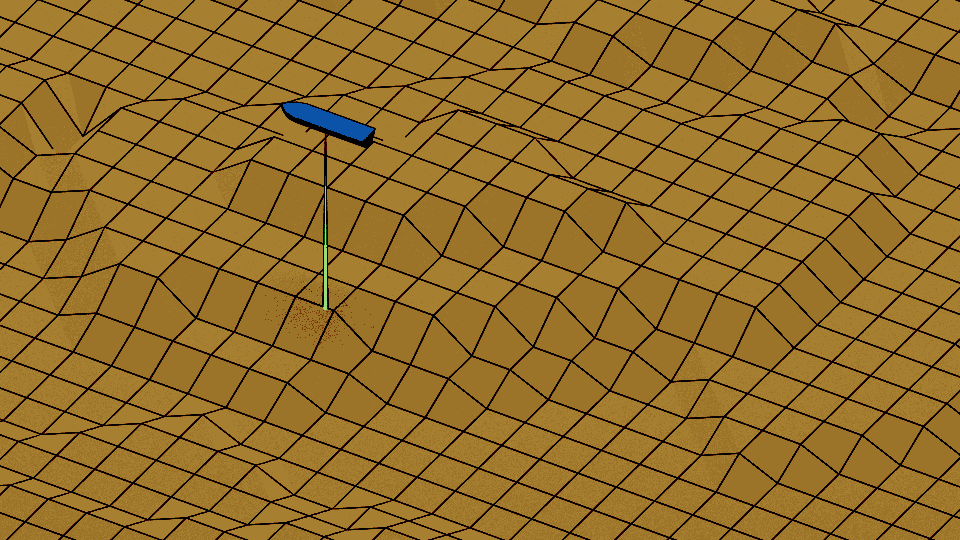
\includegraphics[width=0.48\textwidth]{fig/conseptart-single}}
	\ % One forced space to seperate figures
	\subfloat[Thee ships\label{fig:concept-art3}]{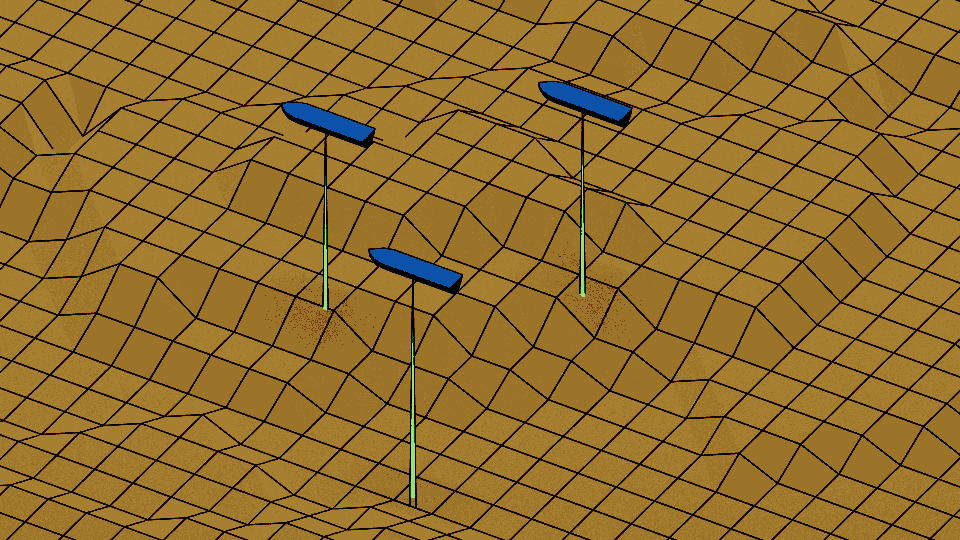
\includegraphics[width=0.48\textwidth]{fig/conseptart-formation}}
	\caption{Comparison of two ways to cover an area with a lawn mower
	pattern.}
	\label{fig:concept-art}
\end{figure}

When only one ship (figure~\vref{fig:concept-art1}) need to map a complete seabed this process could
take up much time dependent on the area that need to be covered. The
time spend could be improved to make this mapping more efficient. One
way of optimizing the time used is to add more ships (figure~\vref{fig:concept-art3}) to help map the
seabed. To make the process of this as optimal as possible it could be
of benefit to implement formation control in the specific assignment.

I cooperation with the port of Aalborg, a use case is presented, where we can perform tests of the platform, and use those to compare the performance of our system to their system.
\begin{figure}[htbp]
	\centering
	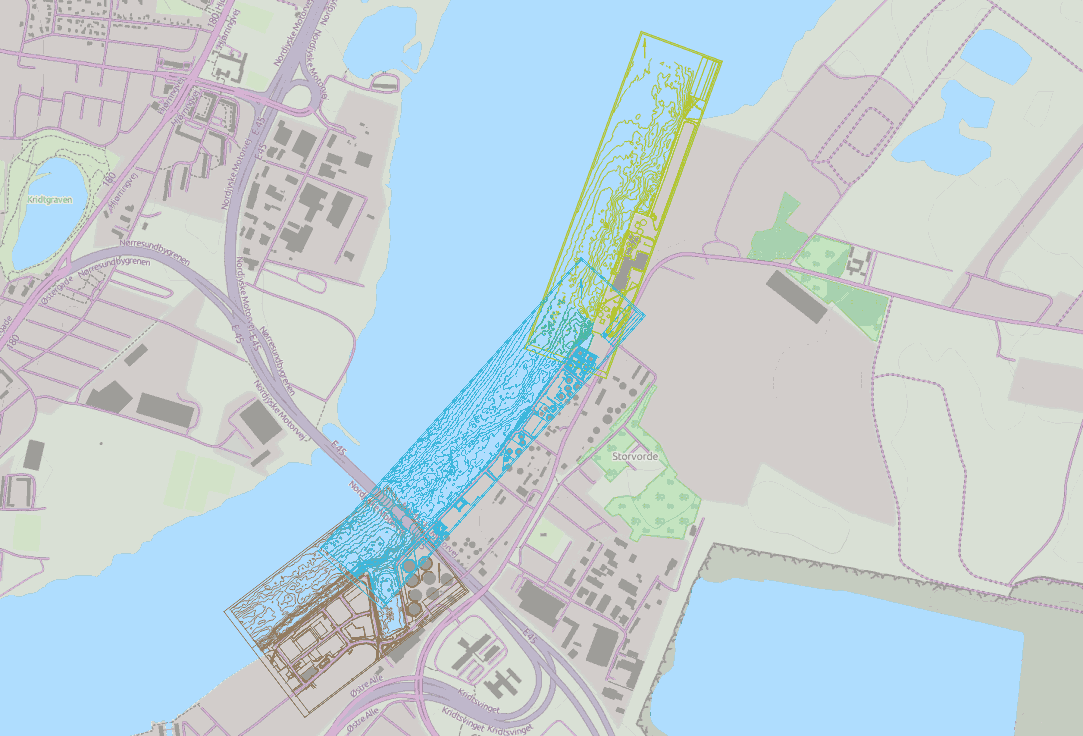
\includegraphics[width=\textwidth]{fig/use-case-data}
	\caption{Area of the harbour at Aalborg Portland provided as sample
	data from Aalborg Havn. Background map data CC BY-SA OpenStreetMap.}
	\label{fig:diffforms}
\end{figure}

When performing this kind of surveying with multiple ships, it is important to take note of the kind of sensor it uses and the coverage that it provides. Initially the port of Aalborg used single beam echo sounders, but have in recent years turned over to multibeam sonars for their survey boat, which has improved their resolution and time for a survey. But they still wishes to improve the survey update rate, by e.g. using fairly low cost autonomous ships to get better indication of the seabed to identify if an expensive thorough survey is needed. An image of the survey vessel they use now used can be seen on figure \ref{fig:alba}. As it can be seen, this survey vessel is relatively large, being over 20 metres long. To comparison is the AAUSHIP only 1.1 metres long. For surveying in smaller areas, like inside the harbour area, Aalborg Havn uses a smaller scale vessel which is 12 metres long. This vessel is only used at the smaller areas thus not the one being used out in the Limfjord close to Aalborg.
\begin{figure}
	\centering
	\includesvg{alba}
	\caption{The survey vessel used by Aalborg Havn named Alba.}
	\label{fig:alba}
\end{figure}



%This could be done in several ways, but is mostly thought of in a
%rigid formation, such that the formation maps the same area of the
%seabed the whole time. The idea can be seen on
%figure~\vref{fig:concept-art}.
 % Talk specifically about the data from havnen?
\chapter{Formation Control Overview}
\label{ch:formcontrol}
\head{This section will give a short introduction to formation control in general, by discussing existing formation control paradigms and relating them to the motivation of the AAUSHIP as a survey platform consept. Some of these concpets will be analysed further in chapter~\vref{ch:selformctrl}.}

%\head{Formation control in general is concerned with simultaneous control of dynamic systems. These systems is often referred to as agents where the objective of these is to maintain a static reference to a specified object. This object could be another agent witch then would be referred to as the leader. The other agents objective will then be to stay in the relative position to the leader within a static formation.}

The theory of formation control in general is widely applied. It is usually applied in assignments regarding control of robots which needs to be placed relative to each other. Depending on the given task of the robots, and which type of robots are in focus, the formation can be utilized in different ways \citep{muv-survey1}.

The robots can also be of various types: Driving vehicles, helicopters, aeroplanes, ships etc. which can be both manned and unmanned. The tasks that these robots needs to fulfill can vary greatly. Robots in groups in general have many purposes such as vacuum cleaning robots, who needs to clean a rather large area or flying swarm robots like quadcoptors who can make different kinds of assignments. When quadcoptors work as a combined group they could lift a certain amount of payload to achieve their goal as a group, or they could work individually in a network to do several smaller tasks. An example of how quadcoptors are working together can be examined at \citep{ethswarm}.

All the robots in the terminology of Zhang and Mehrjerdi are called \textit{agents}. These agents move either individually or in formation. This formation can be rigid or be flexible. If the agents move in rigid formation they will keep their relative positions to each other and must not diverge from the formation. The formation could also be flexible which sometimes is preferable. If the distances between three agents on line are large, and an obstacle needs to be avoided, only one of the agents needs to move from this obstacle if the formation is flexible \citep{muv-survey}. This can be seen on figure~\vref{fig:form_avoid_right}.
\begin{figure}[htbp]
	\centering
	\includesvg[width=0.5\textwidth]{form_avoid_right}
	\caption{A flexible formation where the right agent avoids an obstacle.}
	\label{fig:form_avoid_right}
\end{figure}

\section{State of the art}
When looking into formation control many different types of control can be taken into account. The main types of formation control are separated into six different types, all under the main topic \textit{multiple vehicles coordination strategies}. The overview for this can be found in the survey paper \citep{muv-survey} who explains the six main types and a few alternations of these.

The theoretical views on control of \ac{MUV}'s behaviour are by \citep{muv-survey} divided into two classes; centralized and decentralized systems. If the system is centralized this means that all control of the formation is done on one agent, and the others receive information from the core agent. This form of system has the advantage that the core agent can optimize vehicle coordination, accommodate individual agent faults and monitor the accomplishment of the mission. The main disadvantage of this system is that if a fault should occur in the core agent this will affect and facilitate a failure of the whole system.

The opposite way of controlling the system would be in a decentralized way. This way of controlling the formation is inspired by the aggregation of birds and fish. This makes each agent able to communicate and share information in between. This means that each agent is given its own part of the complete objective and thus can only complete a part of it, like moving around an object to get to end point of a trajectory. The advantage is that faults in a single agent can be overlooked, thus more robust to faults, but can result in a less efficient objective outcome. A decentralized system may be more appropriate to scale up such that more agents can be included and the computational load can, in difference from the centralized system, be split up onto more agents.

The different types of coordination and control algorithms within centralized and decentralized systems include: \textit{behavioural-based}, \textit{virtual structure}, \textit{leader-follower}, \textit{graph-based} and \textit{potential field approaches}. Within these structures are the terms \textit{cooperation control} and \textit{formation control} used. Cooperative control focuses on the global task that the group of agents needs to fulfil, and the formation control is the actions performed by each agent which is shared with the other agents in the group. 
\begin{description}[style=nextline]
	\item [Virtual structure]
	In a virtual structure is the entire formation treated as a single entity. The behaviour coordination for a group of agents in a virtual structure is uncomplicated compared to the coordination of many agents, due to the making of one structure e.g. based on fixed distances between the agents. The disadvantage falls on the centralization due to the structure treated as a single entity. If a failure in this structure happen results in a failure in the entire structure.
	\item [Behaviour Based Methods]
	The behavioural based model employs several behaviours for each of the agents and the final control used to control the formation is derived from a weighting of the relative importance of each of the behaviours. This could for instance be navigational behaviours to enable a navigation to be the main goal while avoiding hazards and stay in formation. So if one agent needs to avoid a collision with an obstacle the rest of the group should not take this into account. Only that single ship needs to leave the formation and get back into formation again.
	\item [Leader-Follower Approaches]
	Applying leader-follower methods designates one agent as being the leader and the rest of the agents as followers. The following agents need to position themselves relative to the leader and maintain a desired relative position to the leader. This makes the simplicity to this method, but there is no feedback from the followers to the leader and thus makes that a disadvantage. Separation-separation and separation-bearing are two popular leader-follower formation controls, where the followers stay at specified separation and bearing from their designated leader. Within this method it is possible to split the group up into several smaller groups with their individual designated leader.
	\item [Potential Field Approach]
	Potential field approaches assigns potentials to agents to make a weighting between them. This weighting could for instance determine the relative distances between the agents. This is usually used when following a virtual leader, such that this process is only made relative to the agents within the structure. This method can make ensure a collision free formation when every agent has been assigned their potential weighting respectively. In this method obstacles can be included and have assigned potentials as well. This will become an avoidance radius from the specific object.
	\item [Graph Theory Approaches]
	When applying the graph theory method one assign every agent as a node and assign connections between the nodes. In graph theory this is denoted vertices and edges. The study with graph theory is mainly concentrated of the formation itself and related to changes within the structure. This can be related to the structure within a tree-structure which is used when assigning the formations in graph theory manor. This can be applied as communication analysis for the agents and consensus analysis can be of benefit. The edges between the nodes symbolizes the possible connections thus communication between them. The nodes that are connected are denoted as neighbours and are capable of communicating.
\end{description}

\subsection{Approaches on formation control}
When performing this kind of surveying with multiple ships, it is important to take note of the kind of sensor it uses and the coverage that it provides. Initially the port of Aalborg used single beam echo sounders, but have in recent years turned over to multibeam sonars for their survey boat, which has improved their resolution and time for a survey. But they still wishes to improve the update rate, by i.e. using fairly low cost autonomous ships.

\missingfigure{Picture of the port of Aalborg's survey boat.}

This does not have any relevant impact of how the mappings of the seabed would be due to the subsequent processing of the collected data from the maps.

Different formations of ships can be seen on figure~\vref{fig:diffforms}.
\begin{figure}[htbp]
	\centering
	\includesvg[width=0.5\textwidth]{diffforms}
	\caption{Different formations which the \ac{ASV}s can make.}
	\label{fig:diffforms}
\end{figure}

The formation of the ships may not need to be strictly rigid. Situations could appear where it would be of benefit to change the ship's formation. If the formation need to avoid an obstacle and one or more ships needs to go faster or slower, which leads to a change in the formation, it might be of benefit to regroup the formation which is faster to reach. An example can be seen on figure~\vref{fig:avoid}.

\begin{figure}[htbp]
	\centering
	\includesvg[width=0.5\textwidth]{form_avoid}
	\caption{A formation needs to go around an obstacle where the inner most ship chooses the shortest path and the formation regroups to a new formation.}
	\label{fig:avoid}
\end{figure}

When doing the formation control it is important to figure out what one
want to achieve, and depending on the strategy and the formation type
some things are to be considered as requirements regarding how the
formation should work. In this discussion lawnmower patterns are considered. In this work thee ships are considered for simplicity, but it should be extensible to n-number of ships. The lawnmower patterns will suit well for the mapping of a seabed where one or more ships are to sail from shore to shore in a fjord.

\subsubsection{Initialisation}
When looking at the specific task several things needs to be taken into account. When starting the mission, the ships may start at positions that is not in the desired formation. It might be of importance that the ships are in
formation when they start tracking the desired track. Therefore some
attention must be given on how to make the ships initialize this
formation. This is referred to as the group coordination task. An approach is to make the ships sail individually to the
starting positions with a speed that makes them hit their respectively starting points at
the same time. If one reaches its start point much earlier
than the other it must stop, which is not wanted because it then can
drift out of position again. This basically means that there exists an initialization
phase and a tracking phase. The start heading should of
course align with the path at the start point such that the path following can begin with zero error. The ships could also target their group formation before starting at time zero at the path. This will eventually make the initialization take longer time but ensure that the ships have made the group coordination task and are ready to start at the path.

Another issue to be considered is to ensure that no ship at
any point in time reaches a minimum speed that is necessary for the
ship to not drift out of formation. This could be a problem in corners
of the formation if a stiff construction, where the inner most ship
has to move slower, to accommodate the shorter distance on an inner
circle arc.

Faults like blackout on a ship could also be considered in the control
design. I.e. what happens with the formation when one ship faults in a
blackout. Should the rest of the formation stop, should the formation
still follow this drifting ship or should the mission simply terminate
when it is discovered that a ship has blackout. This is under the assumption that the formation is decentralized and every ship has its own control and is not controlled from a mother ship.

In the initialization phase it is also relevant to consider how the
ships should avoid each other if they are on the wrong side of each
other. If it is of benefit that a specific ship is at the most inner route, and is located at an outer position before the group coordination, this ship needs to cross the formation to get to the desired starting position. This initialization needs to be adjusted in the initialization phase to ensure that no ships collide.

\begin{figure}[htbp]
	\centering
	\includesvg[width=0.4\textwidth]{cornoring}
	\caption{Two ships initializing and following the path offset
		equally on each side, ships are constrained to sailing parallel
		and heading the same as path when projected onto the path. Blue
	dot is start of path. Fully drawn splines is initializing phase.}
	\label{fig:cornoring}
\end{figure}

On figure~\vref{fig:cornoring} is a simple path following performed
with two ships in a stiff formation with an equal distance from the
path. It illustrates four steps. In step \#0 the ships initializes a
random position near the start of the path being the group coordination task. At \#1 it is tracking the
path in formation, whilst still in formation. This is referred to as a formation coordination task. At \#2, the green
(right) ship is in a tight inner curve where it is important to
consider design of the path such that the capabilities of the ship is not
exceeded to stay in formation. At \#3 it is back to straight line path
following in formation.

\begin{figure}[htbp]
	\centering
	\includesvg[width=0.6\textwidth]{form_rigid_90}
	\caption{Three ships in formation needs to make a 90\textdegree turn and stays in their relative positions and keeps the rigid formation.}
	\label{fig:form_rigid_90}
\end{figure}

When the ships needs to make a turn about something they can do it in many ways. On figure~\vref{fig:form_rigid_90} the ships keep their formation whilst turning about the object. When they reach the other side and have finished their turn, the ships have kept formation but the outer most ship has now become the inner most ship. The reason to turn like this could be that the inner most ship, the yellow ship, cannot turn as sharp as demanded to stay the inner most ship. Therefore, instead of turning the formation, they stay geometrically rigid.

\begin{figure}[htbp]
	\centering
	\includesvg[width=0.6\textwidth]{form_change_90}
	\caption{Three ships in formation needs to make a 90\textdegree turn and changes their relative positions.}
	\label{fig:form_change_90}
\end{figure}

As seen on figure~\vref{fig:form_rigid_90} the ships could have benefit of turning like this. This way of turning could cause trouble in the top of the turn, where the ships eventually will collide due to errors and the relative close distance to each other. This way could be altered a little such that the ships will turn like on figure~\vref{fig:form_change_90}. There the ships adjust their position and velocities to ensure that they will not collide, but they will therefore leave their formation shortly to return back into position again \citep{thorvaldsen}.

\subsubsection{Degree of Actuation}
The degree of actuation is a matter that sets some limitations on how
the path following can be made, and thus the methods available to
control the ships.

AAUSHIP is a ship, which means that is is not fully actuated in the
whole 3D space, but this is not needed since it is moving on a
surface. To be fully actuated it must be able to have controls for
surge, sway and yaw.

There are different ways of controlling, and a few could be:
\begin{description}[style=nextline]
	\item [Three or more controls]
	When having three or more control parameters it is said that the vessel is fully actuated. This way of controlling is usually used in low-speed manoeuvring and stationkeeping mostly by offshore \ac{DP} vessels.
	\item [Two controls and Trajectory-Tracking control]
	Trajectory-Tracking is done in a three \ac{DOF} system, $e(t)\in\mathds{R}^2\text{X}\mathds{S}$. It is done with two control inputs, $u(t)\in\mathds{R}^2$. This means that the control problem is underactuated which cannot be solved by linear control theory. A vessel under these terms is able to manoeuvre along a path with constant sideslip angle using only surge and yaw. This is the classic approach for path following.
	\item [Two controls and Weather-Optimal heading]
	When taking the weather conditions, and in general the environmental disturbances, into account, it is done as a mean of all the disturbances. This is used to stabilize the vessel regarding the position. It is done by making the heading depend of the change in the mean of the environmental disturbances.
	\item [Two controls and Path-Following control]
	The standard way by having two controls, being surge and yaw, and achieving path-following, is to define a 2-D workspace. This workspace is placed along the trajectory with along-track and cross-track vectors that are to represent the error to minimize. This is usually done by applying the \ac{LOS} path following controller that makes use of surge and yaw to accomplish the path following. This implies that a six \ac{DOF} system model needs to be internally stable such that only the two control inputs are used.
	\item [One control]
	This is only done with systems with three \ac{DOF} and is normally only used to stationkeeping.
\end{description}
\citep{fossen}

\subsection{Delimitations}
Within the scope of the AAUSHIP project will the focus be to apply and extend a leader-follower approach at the ships. This will include several tasks. The two main tasks will be to make a group coordination task and a formation coordination task. The group coordination task will be, as described earlier, an objective to get the ships into the desired formation before or exactly at the starting point of the path following. The formation coordination task will be to make a leader, virtual or not, follow a predetermined path set by waypoints. The path should be generated from waypoints placed on a map due to that the ship needs to travel over larger distances. This will make a waypoint based follower where the path will be generated between the placed waypoints.

The placement of the waypoints will be placed such that the ships need to surge along a lawnmower pattern, where the turns have a lower requirement of turn radius dependent on the surge velocity of the most inner ship. This is due to the drift if the inner ship looses too much velocity.

When applying the leader-follower approach it needs to be determined how the formation precisely should be set up. In this project is only one leader considered at a time. The rest of the ships will act as followers to the leader. The idea can be seen on figure~\vref{fig:l_f} where only one leader is represented with a single or more followers.
\begin{figure}[htbp]
	\centering
	\includesvg[width=0.6\textwidth]{lead_follow}
	\caption{A leader is always assigned and potential followers are following.}
	\label{fig:l_f}
\end{figure}
When the followers are in formation with the leader is only the leader who is following a specified trajectory. The other ships, the followers, only keeps their position relative to the leader. This makes the predetermined formation moving along the path relative to how the leader is following the path. The leader is autonomous as well as the followers, but the path following is only done at the leader and the followers maintains their relative positions to the leader.

If the leader diverges from the path, drifting to the left, this will result in the whole formation drifting to the left. This problem can be dealt with in different ways, e.g. the control could react fast enough to make the formation get back on track within a specified time, or some fault tolerance could be done from the whole system. If the leader diverges from the path it could make the formation stay at their respective headings within a time slot before actuating towards the leader.

The formation needs to take into account if it is of benefit to change leader. If some kind of obstacle makes the formation turn about it, it might come to benefit to change the leader which needs to be done on the fly. This entails a change in the group coordination and the ships needs to set their relative position and heading from another ship.

The configuration of the formation will be set up, as a start, with one leader and a single follower. The follower will be offset from the leader with a distance of five metres. This can be seen on figure~\vref{fig:l_f1}.
\begin{figure}[htbp]
	\centering
	\includesvg[width=0.4\textwidth]{lead_follow1}
	\caption{The leader with a follower offset by 5 metres radius.}
	\label{fig:l_f1}
\end{figure}
This will be a rigid formation that the ships needs to keep at all times. The change of leader will eventually be taken into account when the ships needs to turn. If the formation needs to turn clockwise about it might be of benefit to change the leader. 

The location to test and implementation the AAUSHIPs will be in the Limfjord. The optimum will be to make the formation go across the Limfjord and back in lawnmower pattern and make measurements of the seabed. Due to the location where it is presumed to have enough space, the formation is not of bigger importance to the mapping. The only important thing to include regarding the formation is that the ships needs to be able to turn around without loosing so much velocity such that they start drifting and offset the formation.

\chapter{Path Generation}
\label{ch:pathgen}
\head{A guidance system usually consist of a subsystem to generate
	paths for the trajectory which is desired to have the object follow.
	There exists multiple methodologies for this, also depending on the
mission purpose. A description of these methods are described in this
chapter with focus on pre-mission defined paths.}

\noindent For these kinds of guidance systems, they are usually generated via some
form of human interface -- some more intelligent than others. For the
purpose of this thesis, the interest lies in the use of surveying
purposes, such that a path should be generated from some waypoints
that are generated from some polygonal areas of interest.

The concept of this is to make run lines (lawn mover or plough fure pattern) with
straight line segments, and the corners can be handled in a specific
way such that the physical constraints of the ship manoeuvring ability
is considered to generate feasible paths.

There are basically two ways to consider a lawn mover pattern. The
one is to have the area of interest to be covered only by straight line
segments and then end the run lines connected with a turning maneouver outside the
area of interest as show on figure~\vref{fig:lawn-straight-inside}. The other way is to cover the area with all manoeuvers constrained inside the area of interest, where the turns are also included in the area of interest, as illustrated on figure~\vref{fig:lawn-all-inside}.

\begin{figure}[htbp]
	\centering
	\subfloat[Only straight lines\label{fig:lawn-straight-inside}]{\includesvg{lawn_straight_inside}}
	\qquad
	\subfloat[All paths constrained\label{fig:lawn-all-inside}]{\includesvg{lawn_all_inside}}
	\caption{Comparison of two ways to cover an area with a lawn mower
	pattern.}
\end{figure}

\section{Dubins Path}
Dubins path is one way to define paths which can be used in the
context of the AAUSHIP project. The Dubins paths are created by line
segments and circle arcs. These arcs can be created in different ways,
and the usage of this can be applied when generating lawn mover
patterns. The circle arcs can be created from points (waypoints) with
line segments between, like it is intended to do within the AAUSHIP
lawn mover patterns. Different discrete ways to handle Dubin paths can
be found in a summary and discussion with \citep{dubin}. The way the
Dubins path are used in the AAUSHIP is based on the waypoint
terminology, where the vessel needs to go from waypoint to waypoint
connected with a line segment to track onto. This is also one of the
ways that the Dubin paths can be utilized. In the AAUSHIP is the
circle arc defined From a determined distance from between the longer
line segments in the lawn mover patterns. This radius cannot be too
small such that the dynamics of the AAUSHIP does not allow it to go
all around the circle arc without diverge from the determined
waypoints in the arc.
\begin{figure}[htbp]
	\centering
	\includesvg{lawnmoverturn}
	\caption{The figure shows that the spacing between the lines sets the turning radius for the AAUSHIP. This is constrained by the dynamics of the AAUSHIP.}
	\label{fig:lawnmoverturn}
\end{figure}


\begin{figure}[htbp]
	\centering
	\includesvg[width=0.8\textwidth]{normal_dubin_path}
	\caption{An example of a Dubin path generated with straight lines and
		inscribed circles, where the path corner arc radius is determined
	with a minimum radius and dependent on the angle between the two
segments connecting one waypoint to others.}
\label{fig:normal_dubin_path}
\end{figure}


\section{Guidance System}
The guidance system is a system that takes the wishes from the
operator and converts those to some trajectory via a path generating
algorithm. This path generating algorithm will be used to generate the lawn mover patterns for the AAUSHIP to follow. These patterns have been discussed within this chapter. After the waypoints from the operator have been translated into a lawn mover pattern it is up for a tracking algorithm to keep the AAUSHIP at the correct course for the next coming waypoint.

This algorithm can have various purposes and in this project it will be a \ac{LOS} guidance algorithm. This will control the heading of the AAUSHIP such that the vessel will converge to the line segments between the waypoints and afterwards keep the heading at the straight line segment. The guidance system can be one block that keeps the generated track from the waypoints updated, to have the references that the AAUSHIP needs to converge after. This reference is passed on to the control system, which can be seen on figure \ref{fig:losguide}.
\begin{figure}[htbp]
	\centering
	\includesvg{guidance-overview}
	\caption{Overview of guidance system where a mission static waypoint
	database is used as the input to a \ac{LOS} algorithm, which sets
the reference for the ships control system, which is usually
implemented as some form of heading autopilot.}
	\label{fig:losguide}
\end{figure}


\begin{figure}[htbp]
	\centering
	\includesvg[width=\textwidth]{use-case-polygon}
	\caption{Comparison of two ways to cover an area with a lawn mower
	pattern.}
    \label{fig:use-case-polygon}
\end{figure}

Tesselation with quadrilaterals (polygons with four edges and four vertices) is a way to help divide a given polygonal shape into some shape where it is useful to apply a plough fure motion. The shapes of these are equal to how the AAUSHIP needs to move when navigating in a specific area to map the sea bed. It can be done in several ways, where two different can be seen on figure \ref{fig:use-case-polygon}.

%\section{Summary of papers, notes}

\subsection{Vijay Kumar}
\paragraph{A Potential Field Based Approach to Multi-Robot Manipulation}
	Decentralized apporact to planning and control. Hieracial potential
	fields are used to acomplish an objectiv of transporting an object
	in the plane. No absolute positioning is available here. Focus in
	this paper is the automatic formation to surround an object. This
	paper can be used to summarize what potential field based
	approaches is. \citep{pfmrm}

{\vskip0pt\color{gray}
\paragraph{Trajectory design for formations of robots by kinetic energy shaping}
	Rigid formation when doing obstacle avoidance using kinetic energy
	equation. Not really that interresting for us.}

\paragraph{Cooperative Control of Robot Formations}
	Is a book chapter collecting information from multiple papers from
	Kumar. Does some stability analysis with Lyapunov functions, Talks
	about the coordination strategy, which is about changing formation.
	Mentions a strategy where rovers are alloved to collide with each
	other and obstables. \citep{RF:PS:AD:02}

{\vskip0pt\color{gray}
\paragraph{A framework and architecture for multirobot coordination}
	Talks about the CHARON language, not entirely interresting.}

\paragraph{Formation Control with Configuration Space Constraints}
	Using  modified leader follower approach using potential field
	controllers, highly interesting to our goal. This achieves a method
	where it is not only a leader, but a cooperative leader-following.
	This is advantageous if for example some rover cannot keep up with
	the formation. \citep{fccsc}

\paragraph{A Paradigm for Dynamic Coordination of Multiple Robots}
	Using hybrid control to do role coordination of robots, this is a
	formalised approach using a high-level modelling language. It
	enables hierarchies. Still interested in moving objects. It could be
	relevant to look into this, if we are interested in hybrid
	control.  \citep{LC:FC:04}
	
\paragraph{Leader-to-Formation Stability}
	Analysis of formation stability, using graph theory. Could be highly
	interesting for us to determine these properties of a given
	strategy. \citep{TKP04}

{\vskip0pt\color{gray}
\paragraph{Multi-Robot Cooperation}
	Hard to find, not much effort done.}

{\vskip0pt\color{gray}
\paragraph{Cooperative control of UAVs for Search and Coverage}
	Quite interesting, but focuses on motion planning with different
	types of agents, with different sensor systems. This is used for
	surveillance. It considers different constraints for this, these
	are: number of heterogeneous agents, boundary conditions, coverage
	area, keepout zones, sensor footprint mapping and a time budget.}

{\vskip0pt\color{gray}
\paragraph{Critical Cooperative Surveillance and Coverage with Unmanned Aerial Vehicles}
	Cannot be found anywhere, does not exist in the "Experimental
	Robotics: The 10th International Symposium on Experimental Robotics"
	\url{http://link.springer.com/book/10.1007/978-3-540-77457-0}}

{\vskip0pt\color{gray}
\paragraph{Architecture, Abstractions, and Algorithms for Controlling Large Teams of Robots: Experimental Testbed and Results}
	This is a testbed used for testing a decentralized and anonymous way
	for controlling a large team of bonholenomis ground robots. Not
		really what we want.}

{\vskip0pt\color{gray}
\paragraph{Decentralized feedback controllers for Multi-Agent teams in environments with obstacles}
	This is about using decentralized feedback controllers that can
	avoid obstables and collisions. This is not about formation control.}

{\vskip0pt\color{gray}
\paragraph{Cooperative Control of Autonomous Surface Vehicles for Oil Skimming and Cleanup}
	Modelling of the skimmer rope between two boats when towed by two
	boats. This paper describes a method of controlling the shape of the
	rope and tries to maximize skimming efficiency. Not related to our
	form of formation control as such. Could be relevant to describe uses for
    formation control.}

{\vskip0pt\color{gray}
\paragraph{Robust Control of Mobility and Communications in Autonomous Robot Teams}
	About comminication aware control of robot treams with an ad-hoc
	netowrk. This is more like an exploration}

\paragraph{Distributed Multi-Robot Task Assignment and Formation Control}
They focus on the task allocation part of the distribution of assignments for a multi-robot network. They do this in a very specific way which can be interesting to look into, but first after the tasks have been decided. \citep{MicZavKum0805}

\paragraph{Abstractions and Controllers for Groups of Robots in Environments with Obstacles}
This paper addresses the problem of planning and control of single group with homogeneous robots, which is what we have. They focus on obstacle avoidance, but the principle could be used in other methods and might be very useful. \citep{ayanian2010abstractions}

\paragraph{Multi-agent Path Planning with Multiple Tasks and Distance Constraints}
In this paper they deal with a DPC algorithm, which is a Distance something Constraint algorithm. It is made to make timeparameterized constraints on the distances between pairs of robots. They expand this to a multi robot task space, such that the individual robots can, before reaching the final destination, can make a certain amount of tasks defined previously to the mission.
It can be interesting to look into, but maybe only the part about the DPC algorithm. \citep{Planning:ICRA:10}

\paragraph{Distributed Path Consensus Algorithm}
This is an explanation of the DPC algorithm made by Vijay Kumar. It has relevance if we implement graphs to handle the structure of the formation. \citep{bhattacharya2010distributed}

\subsection{Thor I. Fossen}

\paragraph{Formation Control of Underactuated Surface Vessels using the Null-Space-Based Behavioral Control}
This paper concerns a behavioral approach proposed by Thor Fossen. They mainly use the null-space-based approach as an obstacle avoidance, but it can also be used to keep formation. If it is chosen to look at some NSB approach this is indeed of interest. It is a centralized control method. This could be interesting, but maybe only as reference to something else that is possible to implement. \citep{arrichiello2006formation}

\subsection{Steven LaValle}

\paragraph{Time-optimal paths for a Dubins air plane}
This paper considers the dubins path with respect to a modification to the dubins car. This is to generate time optimal trajectories for an air plane, with small radius in turns, straight line segments and pieces of planer elastica.
This is relevant when time comes to look into path generation, so not necessary for us at the moment.

{\vskip0pt\color{gray}
\paragraph{Using randomization to find and optimize feasible trajectories for nonlinear systems}
This focuses on trajectory generation and optimization algorithms for nonlinear systems that have significant state-space constraints.
This is also for path generation, which is not in focus at the moment.}

\paragraph{Algorithms for computing numerical optimal feedback motion strategies}
They compute a navigation function which serves as a feedback motion strategy when looking at the specific constraints, nonconvex collision constraints and optimization of the constraints. They look at the expansion of the state space representation which expands during the expansion of the constraints. The algorithm brings both down in order.
This is also more in focus when we have a strategy to implement by ourselves.

{\vskip0pt\color{gray}
\paragraph{A framework for planning feedback motion strategies based on a random neighborhood graph}
This is, like the others, more a focus on the path planning and how changes in these can be recorrected fast in the navigation function.}


\subsection{Brian Gerkey}

{\vskip0pt\color{gray}
\paragraph{A Framework for Studying Multi-Robot Task Allocation}
Trying to make a framework to the question of “which robot should execute which task?”. They derive a model that helps describe multi-robot systems to provide the common framework in which to study them.
This seems more like a review of how the framework of task allocatin can be generalized and analysed. This it not directly something we need at the moment.}

{\vskip0pt\color{gray}
\paragraph{A formal analysis and taxonomy of task allocation in multi-robot systems}
Making a ontop build of the previously and analyses and making "greater understanding" of existing approaches to task allocation.
Goes the same for this as the last - We do not have that much focus on the task allocation at the moment as such.}

{\vskip0pt\color{gray}
\paragraph{ROS: An Open-Source Robot Operating System}
They discuss how ROS relates to existing robot software frameworks, and briefly overview some of the available application software which uses ROS.
So this was not as I expected and something we already know. \citep{rosoverview}}

{\vskip0pt\color{gray}
\paragraph{Long term autonomy in office environments}
This is from willow garage and they explore options for improving the robustness of robotic systems by identifying failures and executing recovery behaviours, including asking for help from a human operator.
This is not quite what we are looking for, but maybe the robustness of the system and identification of failures can be used maybe for Kevin.}

{\vskip0pt\color{gray}
\paragraph{And all the robots merely Players}
This is also from willow garage. The Player is a middleware for robots, quite similar to ROS, but on a little bit lower level -- sort of. But the Player is a piece of software that are used with some of willow garages hardware and the paper is a history of development of the Player. ROS extends the concept of Player. Not relevant at all.}


\subsection{Raffaello D'Andrea}

\paragraph{Theory and implementation of path planning by negotiation for decentralized agents}
This paper regards path planning algorithms that ensure collision free trajectories in real time. It is robust to delays in the wireless which could be something we need to implement in the connection of the ships where we probably also will experience delay. They have made a hand shaking procedure to ensure recent information states between the agents, which also could be of interest.
The connection as such is not the biggest concern right now where we need to find some formation control strategies.

{\vskip0pt\color{gray}
\paragraph{Coordinating hundreds of cooperative, autonomous vehicles in warehouses}
This "paper" concerns the history and development of machines to the warehouses and stuff like that.
Not relevant at all.}

{\vskip0pt\color{gray}
\paragraph{A decomposition approach to multi-vehicle cooperative control}
This paper focuses on the task allocation problems and has the point of view from a game theory in respective. They make a branch and bound solver which finds near optimal assignments for the robots.
This is still a lot of task allocation and not needed.}

{\vskip0pt\color{gray}
\paragraph{Distributed control of heterogeneous systems}
This paper concerns control design for distributed systems where the controller preserves the distributed spatial structure of the nominal system. Thus this focuses more on the individual system.
This is not that relevant at the moment.}

{\vskip0pt\color{gray}
\paragraph{Distributed control of heterogeneous systems interconnected over an arbitrary graph}
Deals with output feedback controller with H infinite performance for systems composed of different sub units where the underlying graph structure is arbitrary.
This can be relevant when we look at the structure of how the formation needs to shape, but not as much in the formation control aspect.}

\paragraph{Near-optimal dynamic trajectory generation and control of an omnidirectional vehicle}
This paper has also highly focus on the trajectory generation algorithms. This has focus of this with respect to omnidirectional vehicles.
Like the other trajectory generating papers, this has not so much influence at the moment.


\subsection{Howie Choset}

{\vskip0pt\color{gray}
\paragraph{A Complete Multirobot Path Planning Algorithm with Performance Bounds}
The paper deals with multirobot path planning where they decrease the configuration space by couple the relevant robots to each other. In our case we have already done this, because the two or three ships all are in the configuration space.
Therefore this paper is not that useful when we do not have more ships.}

\paragraph{Development and Deployment of a Line of Sight Virtual Sensor for Heterogeneous Teams }
In this paper they develop a 'virtual sensor' that holds information to verify if the LOS is available. It contains more references on first page to some formation control that can be interesting. But it makes the basis of the communication between the robots and how they should exchange information.
This can be useful for us, since it both have references to formation control and has focus on the communication aspects.

{\vskip0pt\color{gray}
\paragraph{Multi-Agent Deterministic Graph Mapping via Robot Rendezvous }
This paper builds on top of SLAM which is not in the scope of the project at all.
Not relevant at all.}


\subsection{Lynne E. Parker}

\paragraph{Multi-Robot Task Scheduling}
This paper contains scheduling problems regarding single robot tasks and multi robot tasks. As I see it, this is mainly based on individual different tasks, but the scheduling part can be used. It considers how the robots should choose assignments, which might be based on how the individual states of the ships are in the current steps.

\paragraph{A decentralized architecture for multi-robot systems based on the Null-Space-Behavioural control with application to multi-robot border patrolling}
This is a cut from Springer and takes into account a lot of aspects regarding both requirements, assumption and control architecture. This seems like a good place to read all. Their focus point is the architecture of the tasks performed by the robots that are separated into three layers; lower layer with the single robot performing its mission, middle layer with definitions of elements of behaviours, which are combined with the Null Space based Behavioural method, the upper later is a Supervisor level selecting the proper action to be executed. It is on 22 pages, so a lot of information.

\paragraph{Behavioral Control for Multi-Robot Perimeter Patrol: A Finite State Automata Approach}
This paper makes a more practical implementation of the Null Space based Behavioural approach that that above mentioned section from Springer explains about. They develop a fully decentralized algorithm for multi robot bovrder patrolling in the framework of the NSB.
This might be good after looking in the 'paper' from Springer, the above mentioned.

{\vskip0pt\color{gray}
\paragraph{Distributed Intelligence: Overview of the Field and its Application in Multi-Robot Systems}
Looking at distributed intelligence and the importance of choosing the right paradigm for this. Dependent on which paradigm chosen, there are use of different task allocations. The paper describes the importance of this, based on the requirements from the system.
The last mentioned is the most important, but nothing that we already knew.}

\paragraph{Current Research in Multirobot Systems}
This paper is a short survey with 8 different topics implemented in physical robots. The interesting topics for us are communication and architecture.
But these seem to be described in other papers also and with a more in depth analysis.

\paragraph{Techniques for Learning in Multi-Robot Teams}
This are some chapters from a book where L E Parker is co author. It describes the adaptive learning in multi-robot systems and the research of time. It focuses on several aspects, but three more that the others. One of them are the learning of inherently co-operative tasks, tasks that cannot be broken into distinct subtasks. The summary tells about the the aspects in assembly robots but then expands and deal with the multi-robot systems.
This is somewhat relevant for us, but not related to the formation control aspect as such for now.

\paragraph{A Distributed and Optimal Motion Planning Approach for Multiple Mobile Robots}
The paper looks at the path planning and velocity planning to a trajectory. They use a search method called D* based on either geometric formulation or schedule formulation. They try to implement this in a distributed manor regarding centralized and exhaustive computation and distributed implementation without optimization concerns.
This is also more relevant after the formation has been determined.

\paragraph{Cooperative Leader Following in a Distributed Multi-Robot System}
This paper is very relevant and deals with the leader follower approach. They both describe design and implementation of a distributed technique to coordinate team level and robot level behaviours. They set up different tasks both for the individual robots and the team as such to describe the tasks.
This seems as a good paper that deals with some of the aspects that we also need to consider.


\subsection{Sebastian Thrun}

{\vskip0pt\color{gray}
\paragraph{Collaborative multi-robot exploration}
The paper has the focus on coordinating robots that need to explore a certain area. There are not in formation, so it optimizes based on time used and other stuff. But this does not seem so interesting because it is not a formation that are used, at least not a very rigid one.}

{\vskip0pt\color{gray}
\paragraph{Integrating grid-based and topological maps for mobile robot navigation}
In here is described two "major" paradigms for mapping indoor environments, gridbased and topoligical. This seems at the moment not relevant.}

{\vskip0pt\color{gray}
\paragraph{Planning with an adaptive world model}
This paper is about obstacle avoidance and is not so relevant. There are also many black boxes in the paper, so not all information is there.}


\subsection{Roland Siegward}

\paragraph{Path Planning, Replanning, and Execution for Autonomous Driving in Urban and Offroad Environments}
The work of this paper is about a single robot, a car, that needs to drive by itself. The focus is on the path planning and following the path. This can be relevant for us to look at, but at the moment not relevant regarding the formation control aspect.
 % should only be included as is in the draft


\descpart{System Design}{%
This is the main part of the report documenting all the engineering that is essential for the project.}
%\chapter{Different Control Strategies}

\head{"A control system, that forces the system output $y(t)$ to track a desired output $y_d(t)$ solves a trajectory tracking problem" \citep{fossen}}.

\todo{Should this be included under the selecteed formation control strageties?}

\section{Trajectory Tracking Control}
When applying control to a vessel that needs to track a specified trajectory, then the type control will be classified according to the number of available actuators.This is usually split between surge, sway and yaw, which corresponds to forward motion, sideslip and turning.

A time varying reference trajectory for a vessel to track will be given as:
\begin{align}
\eta_d=
\begin{bmatrix}
N_d(t)\\
E_d(t)\\
\psi_d(t)
\end{bmatrix}
\end{align}
To achieve tracking and convergence to such a trajectory is minimization of the error the main objective, $e(t):=\eta(t)-\eta_d(t)$. Or given by the previous notation:
\begin{align}
e(t):=
\begin{bmatrix}
N(t)-N_d(t)\\
E(t)-E_d(t)\\
\psi(t)-\psi_d(t)
\end{bmatrix}
\end{align}

When designing a motion control system with this type of objective it is important to distinguish between the following three important control objectives:
\begin{description}[style=nextline]
	\item [Setpoint regulation]
	This is the most basic way of regulating. In this method it is usually a human operator that controls the setpoint or reference to the vessel. The controller will then be a regulator that usually brings the error of the control signal and the real value to zero.
	\item [Path-following control]
	The path-following control makes the vessel follow a path independent of time with no temporal constraints. The method is usually used on underwater vessels or vessels in transit between continents.
	\item [Trajectory-tracking control]
	When applying trajectory-tracking control, position and velocity of vessels should track the position and velocity of some time varying path reference signal. The feedback is a trajectory tracking controller to make the vessel converge to the trajectory. This is used when having course changing manoeuvres and speed changing along the trajectory. This could for instance be a change of speed in a turn of the vessel.
\end{description}

\subsection{Manoeuvring the Vessel Using the LOS Method}
Path-following problems for vessels are often solved by implementing \ac{LOS} algorithms. Opposite to other position control algorithms, where the vessel may be driven both in longitudinal and transversal directions to converge to a path, the \ac{LOS} algorithm gives a more natural motion towards the desired path. This is done by giving a more natural reference to the heading of the vessel. One of the advantages of this is that it can be applied both to fully actuated and under actuated vessels.

Since it is only the leader, and not any of the followers, who need to follow a path, this is only applied on one vessel. This can also be extended to a leader in a virtual structure. To apply the \ac{LOS} algorithm a setup is needed. To get an overview of the functionality of the \ac{LOS} algorithm see figure~\vref{fig:allinallframes}.
\begin{figure}[htbp]
	\centering
	\includesvg[width=\textwidth]{allinallframes}
	\caption{A vessel placed beside the path and uses the \ac{LOS} algorithm to get back on track.}
	\label{fig:allinallframes}
\end{figure}
On the figure is a green vessel that needs to get onto the blue path. The red points at the path is way point positions $\theta$, $\textbf{p}_d(\theta)$. From this point a tangent to the path is made, which crosses the vessels heading and is along the path. The angle from north to the tangents slope (the path) is the \textit{desired heading}, $\psi_d$, for the vessel. This will make it converge to the reference path over time. $s$ along the tangent is the \textit{along track error}(tangential to path) and $e$ from the vessel to the path is the \textit{cross track error}(normal to path), which are two distances that needs to be minimized to make the vessel converge to the path. The along track error is not of great interest when applying a \textit{lookahead-based steering} where only the cross track error is of importance. The lookahead distance along the track is denoted $\Delta$ and is the distance from the normal at the path to the point of \ac{LOS} at the path.

\subsubsection{The \ac{LOS} Algorithm}
The vessel has a generalized position in the ${n}$-frame given as
\begin{align}
\eta = (\textbf{p},\psi)^\top\quad , \quad \textbf{p} = (x,y)^\top
\end{align}
with dynamics given by
\begin{align}
\dot{\eta} = \textbf{R}(\psi)\boldsymbol{\nu}
\end{align}
where $\boldsymbol{\nu} = (u,v,r)^\top$.\\
The path can be parametrized by a set of points with
\begin{align}
\mathcal{P} = {\textbf{x}}\in\mathds{R}^2 : \quad \exists \theta \in \mathds{R} \quad s.t. \quad \textbf{x} = \textbf{p}_d(\theta)
\end{align}
where $\textbf{p}_d(\theta) := (x_d(\theta),y_d(\theta))^\top$ is a smooth function. The path needs to be smooth such that the \ac{LOS} algorithm makes the vessel converge to the path. When applying the \ac{LOS} algorithm it makes the setup immune to sideslip error. This is due to the minimization of $e$ when the vessel approaches towards the path.

For a given value of $\theta$, being a specific point on the path, is the tangent to the path introduced with origin located in $\textbf{p}_d(\theta)$. The orientation of the reference frame, being the desired heading, is given by
\begin{align}
\psi_d(\theta) = \arctan2\left(\frac{y_d^\theta(\theta)}{x_d^\theta(\theta)}\right)
\end{align}
which then will be
\begin{align}
\psi_d = \arctan2\left(\frac{E}{N}\right)
\end{align}
The position of the vessel from the orthogonal position on the path is given in path-tangential coordinates according to
\begin{align}
\epsilon(\textbf{p},\theta) = (s(\textbf{p},\theta),e(\textbf{p},\theta))^\top
\end{align}
where $s(\textbf{p},\theta)$ is the along track error and $e(\textbf{p},\theta)$ is the cross track error. These are given on figure~\vref{fig:allinallframes}, and is the errors from the vessel to the desired point on the path. This position can also be expressed using the rotation of the $\epsilon$-vector by
\begin{align}
\epsilon(\textbf{p},\theta) = \textbf{R}_{2D}(\psi_d(\theta))^T(\textbf{p}-\textbf{p}_d(\theta))
\end{align}
where
\begin{align}
\textbf{R}_{2D}(\psi_d(\theta)) = 
\begin{bmatrix}
cos(\psi_d(\theta) & -sin(\psi_d(\theta)\\
sin(\psi_d(\theta) & cos(\psi_d(\theta)
\end{bmatrix}
\end{align}

\chapter{Selected Formation Control Strategies}
\label{ch:selformctrl}
\head{This chapter investigates the previously mentioned formation control \todo{ref to seciton here} aspects with focus in three different types of formation control. These three types are analysed with focus on the specific task applied at the Port of Aalborg, afterwards simulated to be able to conclude which of these are the most beneficial to implement at the AAUSHIP fleet.}


\section{Relevant Characteristics}
To have a tool to determine what strategy is the best suited for the
problem described in \vref{sc:mission}, some parameters that describes
different characteristics of a strategy is needed. Listed here is a
description of each key parameter, also mentioning what is desired for
the mission at hand. The characteristics are weighted on a scale from $-3$ to $3$ to be able to pick out the relevant formation as a conclusion.

\begin{description}
\item[Communication] The communication requirements should be a measure of how much bandwidth is used. If the communication bandwidth usage is low it should be rated as a good thing, since the low bandwidth implies that the communication can be performed more easy and the scalability will become less complicated. It is not of importance if the communication breaks a link of the agents, this will be discussed in the individual formation control categories. If the communication has a score of $3$, this implies that the bandwidth usage is low and if the score is $-3$ means that the bandwidth usage is high. If only one way communication exists this will probably also lead to lower communication, thus also making a higher score.

\item[Control architecture] The control architecture is a weighting of the complexity of the control structure. A high weighting will mean that the complexity is low and thus less complicated to implement. It will also be combined with a relation to the type of controller, where a more simple controller can be better if the overall objective can be accomplished. If the control can be done with a less complicated controller, i.e. a \ac{LOS} controller instead of some a more complex controller like \ac{MPC}, this can be preferred. The amount of needed inputs to the controller will also be a weighting, thus if the numbers of inputs are high this will be weighted low. The weighting of the control structure is a combination of the above mentioned, where a complex controller with high number of inputs will be weighted as $-3$ and a simple controller with low input will be weighted $3$.

\item[Obstacle avoidance] The obstacle avoidance does not have a specific rating in the use case of the AAUSHIP due to the assumption of a open water manoeuvring. This means that the weighting of this should be taken as neutral and the implementation will be further work. Yet it is described in the specific control strategies because the implementation of this can be useful in the further work of the AAUSHIP projects. The obstacles can be known pre mission or they can be detected during mission and avoided and the task of the avoidance will take different shapes dependent of the specific task. The weighting will be made such that if the obstacle avoidance is easy to implement, it will be weighted $3$, and if it is not present it will be weighted $0$. The reason why no obstacle avoidance is weighted as $0$ is because the criteria does not include obstacle avoidance, but the further work has a weighting to implement it.

\item[Transients] The transients will be a weighting of how well the formation can make a turn and meanwhile keep the formation relative to the path. If the formation are unable to track the path during a turn it will be weighted low ($-3$) and will be the primary weighting. If the formation are able to track the path, but the formation will deviate a little, this will also be a down rating but not as much as if it is unable to track the path. This will i.e. get a weighting of $1$. If the formation tracks the path perfectly and the formation is kept rigid through the transient the weighting will be $3$. Some formation problems during transients can be solved by the generation of the path but this will result as a limitation to the path generation. 

\item[Scalability] The weighting of the scaling is done on two criteria. It is a combination of the structure of the complete formation and the control architecture and an estimate of the bandwidth usage from the higher need of communication. This weighting will be a summed weighting, thus both bandwidth and formation complexity is weighted equally. A rather simple expansion of the formation structure will be preferable, and a relative low bandwidth usage is good. If only communication from a single leader to one respective follower is required, this will be a good thing because it leads to half the bandwidth usage. If the bandwidth usage is high and the control architecture is complex this will lead to harder scalability, which in that case will be weighted $-3$. If the control architecture is low and the input to the controller is low, the bandwidth is low and the communication layer is simple this leads to simple scalability which will be weighted $3$.

\item[Failure]
The failure criteria in these topics are only related to the output of the failure. It is not of relevance if the failure arises in sensors, in actuators or in the control structure, but only what will happen to the mission if one agents fails out. The degree of what will happen will choose the weighting such that if one agent fails and every other agent also fails the mission, this will be weighted as $-3$. If a single agent fails and nothing else happens will lead to a weighting as $3$, because if an agent will fail and the mission still can be completed it is preferable.
\end{description}

There are also some parameters that is hard to tell by the principle
of the method, which is listed below. These can be used to compare the
strategies after implementation.
\begin{description}
\item[Preparation time] This is related to the mission setup time. How
	much manual labour is needed to prepare the agents for a mission?
	This could for instance be trajectory generation and how the
	specific pattern needs to be generated. If the formation control strategy is chosen such that the agents needs to be close to the specific formation this will also take preparation time to place them relative to the desired formation.
\item[Time] The mission time for covering the area in a boustrophedon
	pattern. This will be from the start of the mission to a complete mission.
\item[Energy efficiency] This is a theoretical measure of the
	formation efficiency. The energy efficiency of any autonomous systems is relevant because it limits how long the autonomous system can operate autonomously, given that it cannot easily recharge or is fatal for the mission. This means that optimising the energy efficiency is desirable.
\item[Wear and tear] Is the controller aggressive? Aggressive
	controllers is known to make more wear and tear on the actuators. So
	if the strategy can be chosen to minimize the wear and tear this
	could be of benefit to the hardware.
\end{description}

%% Oversigt af control stats

\section{Methods}

\subsection{Direct LOS guidance}
The \ac{LOS} guidance makes the basis for a formation where one leader has a single follower connected and this follower has another single follower. \todo{Her skal nok stå en overordnet beskrivelse..}
\subsubsection{Duckling formation}
\label{sc:duckling}
This strategy takes the rise in a duckling or snake formation. In principle is this a leader that has a follower that has a follower and so on. Thereby will the formation take shape as a snake, when the leader takes off and the followers keep the line of sight to their respective leaders. The communication needed in the case of followers only follow one leader, and the communication only works in one direction, then the bandwidth usage is minimal. This implies that the communication it low and simple which is preferable. Similar to the communication will the control architecture become of the simple type where each agent only need to have a \ac{LOS} controller, such that they track their respective leaders. As such is obstacle avoidance not a native implementation of the formation, but can be implemented for the main leader of the formation. By doing this arises a problem of transients where the followers will 'cut corners'. They will directly pursuit their respective leaders, such that the formation will take sharper corners than the main leader. Adding to that if one agent fails during mission every agent after this in the chain fails. Although the formation does not perform well it has the advantage that the scalability is simple. When linking the formation in the duckling formation a new follower can be attached at the last agent and a new follower to this agent and so on. This implies that, in theory, an infinite tail of followers can be attached.

\subsubsection{Echelon formation}
The echelon formation is a branch from the duckling formation. In this formation the followers to the leader is not in a tail of the leader, but is offset into a echelon formation. The principle being the simple \ac{LOS} controller and the communication as followers to their respective leaders still apply in this branch, but the reference is given to the followers as a offset with an angle and a degree. This implies that the problem statements from section \ref{sc:duckling} also applies to the echelon formation, and the main difference is the shape of the formation and how the reference is passed on.

\subsubsection{\ac{FRP} with path}
This method only makes use of one path for the whole formation. The agents in the setup will be defined with relative positions to a \ac{FRP} at each time step, such that the formation stays rigid and the arms from the \ac{FRP} to the agents are constants. This setup will in principle work as the followers working in a rigid formation where only the point on the path (the \ac{FRP}) determines where the agents need to go. The reference given to the agents will be a position in the \ac{FRF}, and the formation will have the origo (turning point) in the \ac{FRP}. The individual agents will not be able to communicate, due to the rigid formation, but only keep the position relative to the \ac{FRP}. If the formation stays rigid during transients there will be no problem with collision. If one single agent in the \ac{FRF} fails it will just fall out of the formation and the rest will continue the mission.

\subsection{Precomputed individual paths}
\subsubsection{Full communication}
The implementation of this strategy needs to know for each time step for each agent when the goal at the trajectory is. By doing this it is possible to make the agents be in formation at all times because they have individual positions at their respective paths to specific times. If one of the agents does not reach its position in time, the rest of the agents should stop, or slow down, such that the missing agent has the possibility to catch up. This will change the 'time goals' for the rest of the agents, but the agents will keep the formation. The other option is that the slower agent speeds up, if the agents are not already working at full speed. In this formation principle every agent needs formation about where the others are, which might not be preferable when looking at the bandwidth usage and the scalability of this principle. The same problem will arise when looking at the control architecture, which will only expand more and more when adding more agents. If every agent needs to know information for the others, and act dependent on every single other agent, then the decision and the task allocation will become more complex. When looking into the problem of transients and 'cutting corners', the strategies with individual paths does not have any problems with this. If the formation does cut corners and fail in transients, it is mainly a design error of the path, such that the paths intersect each other. If one of the agents fail during mission then rest will keep close to that agent, unless some kind of exception handling has been made, such that the rest can continue the mission.

\subsubsection{Limited communication}
The overall principle of this implementation is the same as when full communication, the one mentioned above. The difference is that the communication will be greatly decreased when looking at the bandwidth usage and how many agents that needs to know of each other. In this formation strategy agent $i$ only knows information about the neighbour agents, $i_{-1}$ and $i_{1}$.By doing this the information about a slower, or even failed, agent needs to propagate through the formation. If the formation is relatively small, it will not make any remarkable change in the formation structure. If the formation is of a larger size, then the formation will not be as rigid as the one with full communication. If the outer most agent for some reason slows down, then the neighbour needs to act according to that, and the the neighbour of the neighbour needs to act according to that and so on. This will make the formation, in this situation, become skewed, but will go into formation again over time. This is a downside when looking at the transients of the formation and how rigid it is. If the given agent completely fails the mission and breaks down, then the same applies as if there were full communication. An exception needs to be programmed such that the formation will leave the failed agent. The advantage of this strategy is that the control architecture and the communication level will become less complicated, and the scalability to in theory infinitely many agents becomes possible.

\subsubsection{No communication}
Again is the main principle the same for this strategy, only that no information is shared between the agents. If no information is shared between the agents it is assumed that they do not experience any faults. If one of the agents has a fault, that it changes course, slows down or fails in the mission, it will make the formation to fail. The individual agents will still follow their respective paths, and therefore reach their end goals, but not at the same time. If the agent has failed the mission the others does not take this into account, but instead continues their individual mission. The communication in this strategy is very low, since the agents does not exchange information at all. The control architecture also becomes less complex while this strategy only controls the individual agents i.e. with a simple \ac{LOS} controller to track their individual paths. If the individual paths have been generated properly there should not be any problems relating the transients, if assumed that every agent follows its path with acceptance. If it does not, and deviate a little, the formation is not rigid. If one agent fails in the mission, it will also lead to formation deviation, but the rest of the agents will keep their respective goals. Though when working as individual agents, this also implies that the scalability becomes less complex because the control is applied at the individual agent that follows its own path.

\subsection{Potential field}
\subsubsection{Full communication}
In the strategy with potential fields the level of communication can also vary. If the communication can be shared by all the agents within the potential field, the communication is said to be full. When this is the case, every agent has the information about every other agents position and potential field. This makes the formation, made by the potential field, able to correct if any agent starts to fall behind. This concept is the same as with the precomputed paths, where the communication also could be full. In this case the bandwidth usage is also larger when having full communication than with lower communication. Therefore is the communication level also more complex then every agent needs to exchange information with each other. When every single agent need to be dependent on all the other agents, the constraint level gets higher and the complexity of the needed control architecture also becomes higher. When every agent knows the potential fields of the others there should not become any collision problems in transients. But the formation in general is not as rigid when working with potential fields, because of the principle of attraction and repelling. If one single agent fails, breaks down, the others should still know of its appearance such that they can use the potential field to manoeuvre away from the agent. This is mainly to avoid collision. When the communication and the control architecture becomes more complex under full communication, the scalability also becomes more complex. It is not impossible to scale, but a scaling in theory to infinity will become very complex.

\subsubsection{Limited communication}
When the communication is said to be limited it means that not all agents can communicate with each other. The communication range of the agents are reduced, such that i.e. agent $i$ only can communicate with agent $i_{-1}$ and $i_{1}$, but the range can also be large, $i_{-r}$ and $i_{r}$, where $r$ is the communication radius. When doing this the same thing will happen as in the case of limited communication with the individual paths. If one agent starts falling behind then the nearby agents starts to reach first, which then leads to that all agents will reach on the slower agent. Dependent on the formation this will make different hurdles. The formation can try to manoeuvre dependent on the slower agent, but they meanwhile have to follow the potential field map, the given trajectory. In the case of limited communication the same things apply to transients as when full communication, but the formation might diverge more from the determined due to the passing of information between the agents. If one agent breaks down the same goes as with full information, because only the closest agents needs the information about the breakdown to avoid collision. The rest can still continue the mission afterwards. The scaling of the formation becomes a little less complicated than if the agents needed to know information from every agent. Though the potential field mapping will still be complex, and the trajectory generation can be hard.

\subsubsection{No communication}
In the case where no communication are to find in the system the agents will act like no potential field exists from the other agents, and try to follow the potential field trajectory. This will make every agent, independent of the others, try to follow the trajectory and thereby be in the same point. This will over time make the agents collide, if not on the way to the mission goal then at the mission goal. This means that in this case they need a individual potential field trajectory. When making individual potential field trajectories will the scenario be as in the case of individual paths, where the agents will be controlled individually but with respect of a potential field trajectory. This may also lead to colliding agents but it is not necessary as it will be if they followed the same trajectory. If they follow the same reference trajectory a failed agent will result in all the others following behind that will collide resulting in a complete mission failure. Though if the agents instead have their own respective reference trajectory one failing will not fail the mission. If the formation are unlucky, they can collide, but not necessarily.

\begin{sidewaystable}
\begin{tabular}{l|lll|l}
\toprule
\textbf{Approach} & \textbf{Communication} & \textbf{Control architecture} & \textbf{Obstacle avoidance} & ---\\
\hline
\textbf{Leader follower:}&&&& \\
Duckling & Simple, 3 & Simple LOS, 3 & None, 0 & \\
Echelon & Simple, 3 & Simple LOS, 3 & None, 0 & \\
\ac{FRP} with path& Low communication, 0 & Simple, 2 & None, 0 & \\
\textbf{Precomputed individual paths:}&&&& \\
Full communication& High bw, 0 & Multi agent info, 0 & None, 0 & \\
Limited communication& Middle bw, 1 & Local agent info, 1 & None, 0 & \\
No communication& Low bw, 2 & Single agent info, 2 & None, 0 & \\
\textbf{Potential field:}&&&& \\
Full communication& High bw, 0 & Multi agent info, 0 & Natural, 3 & \\
Limited communication& Middle bw, 1 & Local agent info, 1 & Natural, 3 & \\
No communication& Low bw, 2 & Single agent info, 2 & Natural, 2& \\
\bottomrule
 & \textbf{Transients} & \textbf{Scalability} & \textbf{Failure}& \textbf{Sum}\\
\hline
\textbf{Leader follower:}&&&& \\
Duckling  & improper path, -1 & Easy duplicate, 3 & 2 & 10\\
Echelon  & Improper path, 0 & Easy duplicate, 3 & 2 & 11\\
\ac{FRP} with path   & Improper path, 0 & 2 & -2 & 2\\
\textbf{Precomputed individual paths:}&&&& \\
Full communication   & 3 & -1 & 2 & 4\\
Limited communication  & 2 & 1 & 0 & 5\\
No communication   & 1 & 3 & -2 & 6\\
\textbf{Potential field:}&&&& \\
Full communication  & 3 & 0 & 2 & 8\\
Limited communication  & 1 & 1 & 2 & 9\\
No communication  & -1 & 3 & -1 &7\\
\bottomrule
\end{tabular}
\caption{Decision matrix for the formation strategies. The strategy row from the upper half of the table continues on the lower half, with the points summed in the last column in the lower half.}
\label{tab:decision-matrix}
\end{sidewaystable}

The sum is based on the above mentioned categories and is a weighting from $-3$ to $3$ including $0$. The focus will be placed on the three strategies that scores the highest rating. These can be seen in table \ref{tab:decision-matrix} to be \textbf{Duckling formation}, \textbf{Echelon formation} and \textbf{Potential field formation}. The duckling- and echelon formations have achieved the high rating due to their simplicity and their relatively easy implementation possibilities, while the potential field formation is of higher complexity but still fulfils the criteria from the analysis. When analysing these three strategies it becomes clear that the difference between duckling formation and echelon formation regarding implementation is not very different. The duckling formation will become a direct intercept from follower to leader, where in theory an infinite number of agents can be attached. These all need to fulfil a distance reference in between to avoid colliding, and a trajectory will need to take wide turns to ensure that the absolute speed of every agent stays above a threshold. If the speed decreases it will lead to the agent over steering thus needs to over actuate in the opposite direction. This will lead to oscillations in the trajectory tracking and a risk of colliding becomes relevant. The echelon formation is an offset between a follower to the leader, where the same applies as for the duckling formation. It is also possible to expand this to an infinite number of agents that couples the formation together. There the agents also need to fulfil a distance reference to withhold the determined distances in between and thus also a speed reference. The last formation is the potential field, which becomes more abstract to interpret. The theory of setting control structures for the potential field is designed of attracting and repulsing forces and be using those also implements obstacle avoidance. The formation strategies are explained in more detain in the following.

%% Approaches
\section{Strategy 1: Potential Field Formation}
\label{sc:potential-fields}
% Papers of interrest to this topic
% A Potential Field Based Approach to Multi-Robot Manipulation \citep{pfmrm}\\
% Formation Control with Configuration Space Constraints, \citep{fccsc}\\
% UAV Formation Flight using 3D Potential Field, \citep{UAVff3dpf}\\


\subsection{Potentialfield}
In potential fields it is commonly used that a multi-robot group should move in an environment, either with or without obstacles, some papers are \citep{pfmrm}, \citep{fccsc} and \citep{UAVff3dpf}. In the environment there need to be specified some relative measurements, or states, such that the robots are capable to manoeuvre relative to something. This reference, that the robots should manoeuvre with, is in this case the potential fields. When looking at robots that should keep distance from each other (in a formation), or should move to a desired position (trajectory tracking), the implementation of potential fields come in handy.

The potential field approach can be utilised or implemented in
different ways when taking about formation control. Potential fields
is often used for cooperative control where the formation between
agents is not as important, but rather have the goal of moving agetns into formation and then make groups of
agents move from one point to another \citep{5504176}. So to
use the potential field mindset it is important to define how these
fields works together to achieve some form of formation that can be
moved after a predefined path. 

Some ideas is to use an individual potential field seen from each
agent and combine this with the other agent's local potential field.
Here the potential field has local minima defining the desired
formation. In addition to this there is also a need to define how this
formation can be moved in a predefined path.

Another idea is to use the same potential field, that is a global and
common time varying potential field to define the formation, but this
will require that the agents are already near their formation, such
that every agent will approach their separate local minimum. This can
be used as a leader follower concept where the leader is defining this
global potential field.

The potential fields can be defined from attraction- and repulsion forces, dependent on if the robots need to move toward or away from a target, described in \citep{pfmrm}, where potential fields are utilized with a virtual structure. When applying a virtual structure the group of robots follow a virtual leader and not another robot relative to the formation. The potential functions can now be used as forces between the agents to repel them, such that they do not collide, which can be called inter-vehicle forces. The potential functions are also used as forces around the virtual leader such that the agents gets as close as possible to the virtual leader without ever reaching it, which can be called virtual leader forces. This will make a defined formation around the virtual leader \citep{1655803}. The repelling forces can be utilized in different ways and with advantage used with obstacle avoidance, where these need to contribute with a repelling force to the potential field, making agents diverge from these objects. A great advantage to the virtual leader is that the potential forces can be used to keep the formation and then only generate the trajectory for the virtual leader and not for every individual agent \citep{1655803}. The virtual can also be an agent as the reference point in the formation but is mostly thought of as the reference point for all agents in the formation.



\section{Strategy 2: Leader-Follower}

The leader follower principle is used as a higher order principle of how to navigate a group of robots. The principle is that a leader is defined to lead the group of robots in an environment relative to a trajectory. Instead of all the individual robots track their respective trajectories, only the leader follows a trajectory and the following robots keep their position relative to the leader position.

The way that the followers maintain their position can be done in different ways e.g. potential fields \citep{pfmrm}, behavioural methods as Null Space Based behavioural methods \citep{arrichiello2006formation} or versions of a direct \ac{LOS} algorithm. With the focus in here the formation should be defined as a 'rigid' formation, where the follower's positions are defined as fixed distances from the leader. The term rigid is not a strict description in this case because the formation can vary a little all the time, but it is not flexible either \citep{976029}.

The positions should be defined individually for each of the followers to the position of the leader. This can be done through a formation constraint function, F($\eta$), which should be a strict convex function to ensure the formation constraint (the actual formation). This formation constraint function can be expressed in different ways, with the actual positions of the agents and the virtual leader or positions of the agents relative to the virtual leaders starting position.

From the decision table \ref{tab:decision-matrix} it can be seen that duckling formation and echelon formation have got a high rating. These are both branches of the leader-follower principle which often shows to be applicable in formation issues \citep{TKP04}, \citep{1013687}, \citep{976029}.

The duckling formation is a direct intercept algorithm, where the followers intercept their respective leaders and withholding a desired safety distance to their leaders. They will form a chain of leader-follower-follower-follower continuing with followers until the desired amount of robots are in the formation. This formation is named duckling since this will be as a family of ducks where the children follow directly after their parents and does not care about anything on their way.

The echelon formation is a branch from the duckling formation where, instead of a direct pursuit, the followers are given a offset from the leader thus spanning the formation. This offset can be given in different ways i.e. with a desired difference in distance in a fixed angle from the leader. In the same way as the duckling formation this also has the opportunity to expand with a desired amount of robots in the formation that follows their respective leaders.

\section{Strategy 3: Multi Path Following}
Multi paths, or individual paths, for the vessels is where the agents follow their respective paths with respect to time along the path. This needs to make a formation for the vessels. They might only need to know from each other how far they are on their respective paths, such that every agent has a time depending factor on the path. If every agent fulfils its time dependency, this ensures, also by design of the path, that no collision will occur. The paths for the individual agents can be designed from the trajectory of the leader with an offset both in distance in a direction and a time. The time dependencies can make the following agents lack in time thus make this formation as a echelon formation, and the distance with a direction spans the formation itself. The different positions for the $i$th agent will then need to fulfil that the position is the desired position at a specific time
\begin{align}
\eta_d(t) = \eta(t)
\end{align}
where the error in position needs to be zero, $e_\eta(t) = \eta_d(t) - \eta(t) = 0$. The same needs to be fulfilled for the heading of the agents
\begin{align}
\psi_d(t) = \psi(t)
\end{align}
where the error in heading needs to be zero, $e_\psi(t) = \psi_d(t) - \psi(t) = 0$. When these two parameters given at the path are fulfilled the group of agents are said to be in formation. This formation strategy will not be tested as it did not get the highest rating from the analysis in the decision table \ref{tab:decision-matrix}. Though it can be a preferable way of designing the formation if the path can be generated to the specific case.

\chapter{Modelling}
\head{This chapter describes the modelling of AAUSHIP. This is
necessary to be able to use model based control algorithms and
estimators.}

\section{Hydrodynamic Modelling}
Hydrodynamic added mass is defined as the mass added to a system due to an accelerating or decelerating body that needs to move a volume of the surrounding fluid as it moves through it. To this is said that the object and fluid is not able to occupy the same physical space simultaneously.
\begin{align}
M_A \dot \nu_r + C_A(\nu_r)\nu_r + D(\nu_r)\nu_r + g(\eta_r) = \tau
\label{eq:hydmodel}
\end{align}
where
\begin{align}
&M_A \text{ is the added mass matrix from the system}\nonumber\\
&C_A \text{ is the added mass matrix due to the Coriolis force}\nonumber\\
&D(\nu) \text{ is both the potential and viscous damping matrices}\nonumber\\
&g(\eta) \text{ is the restoring forces, which is dependent on the position of the vessel}\nonumber\\
&\tau \text{ is control and propulsion forces}\nonumber\\
&\nu \text{ is the velocities of the vessel in all directions and moments}
\end{align}

\section{Rigid Body Modelling}
The rigid body is used to model the physics of the vessel. It is an idealisation of the solid body from where the physical motions of the vessel are to be derived. Translational motion and rotational motion be derived by analysis of this, and by \citep{fossen} written in component form as:
\begin{align}
f^b_b &= [X,Y,Z]^T & &- \text{force through } o_b \text{ expressed in } \{b\}\\
m^b_b &= [K,M,N]^T & &- \text{moment about } o_b \text{ expressed in } \{b\}\\
v^b_{b/n} &= [u,v,w]^T & &- \text{linear velocity of } o_b \text{ relative } o_n \text{ expressed in } \{b\}\\
\omega^b_{b/n} &= [p,q,r]^T & &- \text{angular velocity of } {b} \text{ relative to } \{n\} \text{ expressed in } \{b\}\\
r^b_g &= [x_g,y_g,z_g]^T & &- \text{vector from } o_b \text{ to CG expressed in } \{b\}
\end{align}

The rigid body forces are written as:
\begin{align}
M_{RB} \dot \nu_r + C_{RB}(\nu_r)\nu_r = \tau_{RB}
\label{eq:rigidmodel}
\end{align}
where
\begin{align}
M_{RB} &\text{ is the system inertia matrix}\nonumber\\
C_{RB} &\text{ is coriolis-centriopedal matrix}\nonumber\\
\tau_{RB} &\text{ is a lumped force combined of } \tau_{\text{hyd}} + \tau_{\text{hs}} + \tau_{\text{wind}} + \tau_{\text{wave}}\nonumber
\end{align}
where in $\tau_{RB}$
\begin{align}
\qquad \tau_{\text{hyd}} &\text{ is the hydrodynamic force}\nonumber\\
\qquad \tau_{\text{hs}} &\text{ is the hydrostatic force}\nonumber\\
\qquad \tau_{\text{wind}} &\text{ is the wind force}\nonumber\\
\qquad \tau_{\text{wave}} &\text{ is the wave force}\nonumber
\end{align}

\section{Total Model of Vessel}
\begin{align}
\underbrace{M_{RB} \dot \nu_r + C_{RB}(\nu_r)\nu_r}_{\text{rigid-body forces}} + \underbrace{M_A \dot \nu_r + C_A(\nu_r)\nu_r + D(\nu_r)\nu_r + g(\eta_r)}_{\text{hydrodynamic forces}}  = \tau + \tau_{RB}
\label{eq:totmodel}
\end{align}
\todo{Argumenter via reference til f.eks. fossen at vi kan se bort fra
nogle led. Er det en valid antagelse?}
\citep{fossen} \todo{lav lidt mere præcise refs til fossen som står lige førnævnt} Since the vessel within this project is of smaller scale, the $M_A$, $C_A$ and $C_{RB}$ from \ref{eq:hydmodel} and \ref{eq:rigidmodel} are neglected. $M_A$ is the added mass and is as a start omitted due to the tests needs to be made as an object moving through the water with some drag. If the model needs to be further improved in the process this is a place to start modelling. The coefficients of $M_A$ are rather inconvenient to determine without advanced equipment like a towing tank, where constant velocity can be applied and measure drag and more in all directions and moments. $C_A$ and $C_{RB}$ represents forces due to a rotation of the body frame, \{$b$\}, about the inertial frame, the NED frame. These are omitted as well due to the small vessel where the body frame is placed in a predefined local frame which acts as the NED frame. This reduces equation \ref{eq:totmodel} down to the following:
\begin{align}
M_{RB} \dot \nu_r + D(\nu_r)\nu_r + g(\eta_r) = \tau_{RB} + \tau
\label{eq:reducedmodel}
\end{align}
The damping matrix which contains the coefficients of the drag is denoted the hydrodynamic damping matrix. This consists both of $D$ which is the linear damping matrix due to potential damping and possible skin friction with the water and $D_n(\nu_r)$ which is the nonlinear damping matrix due to quadratic damping and higher order terms. This can be expressed as $D(\nu_r) = D + D_n(\nu_r)$. This will, as a start, be modelled as the linear part, being potential and viscous damping. At higher velocities will the nonlinear part become more dominant due to the quadratic terms of the velocity, thus is mostly used with faster vessels. The linear damping matrix $D$ contributes more at lower speed manoeuvrings and stationkeeping. Therefore is the damping matrix $D$ used, and is expressed by ~\citep{fossen} for a 6 \ac{DOF} system to be:
\begin{align}
D =-
\begin{bmatrix}
X_u & 0 & 0 & 0 & 0 & 0\\
0 & Y_v & 0 & Y_p & 0 & Y_r\\
0 & 0 & Z_w & 0 & Z_q & 0\\
0 & K_v & 0 & K_p & 0 & K_r\\
0 & 0 & M_w & 0 & M_q & 0\\
0 & N_v & 0 & N_p & 0 & N_r
\end{bmatrix}
\label{eq:6dofd}
\end{align}

The rigid-body system matrix of the vessel is given for a 6 \ac{DOF} system by ~\citep{fossen} as:
\begin{align}
M_{RB} &=
\begin{bmatrix}
m\boldsymbol{I}_{3x3} & -m\boldsymbol{S}(r^b_g)\\
-m\boldsymbol{S}(r^b_g) & \boldsymbol{I}_b
\end{bmatrix}
\nonumber\\
&=
\begin{bmatrix}
m & 0 & 0 & 0 & mz_g & -my_g\\
0 & m & 0 & -mz_g & 0 & mx_g\\
0 & 0 & m & my_g & -mx_g & 0\\
0 & -mz_g & my_g & I_x & -I_{xy} & -I_{xz}\\
mz_g & 0 & -mx_g & -I_{yx} & I_y & -I_{yz}\\
-my_g & mx_g & 0 & -I_{zx} & -I_{zy} & I_z
\end{bmatrix}
\end{align}

The restoring forces acting on the vessel, while not in zero angle position in pitch and roll, is given by the coefficients of the $g$ matrix. The restoring forces acts on the vessel when it is perturbed away from the steady state angle in both pitch and roll. Then vessel will, due to Archimedes law, move back into steady state. The change in mass under waterline will rotate back to steady state and the change in angle will become zero. The coefficients in $g$ is the nonlinear terms contributing to the restoring force. Though it can be convenient to use the linear approximation, defined for a 6 \ac{DOF} system by \citep{fossen}, as:
\begin{align}
g(\eta) \approx G\eta
\end{align}
where $G$, for an asymmetric vessel, is defined as:
\begin{align}
G = -
\begin{bmatrix}
0 & 0 & 0 & 0 & 0 & 0\\
0 & 0 & 0 & 0 & 0 & 0\\
0 & 0 & -Z_z & 0 & -Z_\theta & 0\\
0 & 0 & 0 & K_\phi & 0 & 0\\
0 & 0 & -M_z & 0 & M_\theta & 0\\
0 & 0 & 0 & 0 & 0 & 0\\
\end{bmatrix}
\end{align}

This will be reduced to a 5 \ac{DOF} system due to the fact that the
vessels buoyancy cannot be controlled as such. The vessel will always
be on the water surface and this removes the degree of freedom which
is the heave, the change of $z$ position of the vessel. A 5 \ac{DOF}
system will be modelled as;
\begin{align}
M_{RB} =
\begin{bmatrix}
m & 0 & 0 & mz_g & -my_g\\
0 & m & -mz_g & 0 & mx_g\\
0 & -mz_g & I_x & -I_{xy} & -I_{xz}\\
mz_g & 0 & -I_{yx} & I_y & -I_{yz}\\
-my_g & mx_g & -I_{zx} & -I_{zy} & I_z
\end{bmatrix}
\end{align}
and
\begin{align}
D = -
\begin{bmatrix}
X_u & 0 & 0 & 0 & 0\\
0 & Y_v & Y_p & 0 & Y_r\\
0 & K_v & K_p & 0 & K_r\\
0 & 0 & 0 & M_q & 0\\
0 & N_v & N_p & 0 & N_r
\end{bmatrix}
\label{eq:damping-matrix}
\end{align}
and
\begin{align}
G = -
\begin{bmatrix}
0 & 0 & 0 & 0 & 0\\
0 & 0 & 0 & 0 & 0\\
0 & 0 & K_\phi & 0 & 0\\
0 & 0 & 0 & M_\theta & 0\\
0 & 0 & 0 & 0 & 0\\
\end{bmatrix}
\label{eq:restoreforce}
\end{align}
where the heave are neglected from the 6 \ac{DOF} system. In the principle could a 3 \ac{DOF} system be enough to make the control to the vessel and make it manoeuvre in the water, but as the scope is to exploit the sonar to map the seabed it would be beneficial to implement the roll and pitch as well and make the system as a 5 \ac{DOF}. The $G$ matrix has been reduced under the assumption that there exists yz symmetry, which is a good assumption based on the design of the vessel.

\section{Identification of Hydrodynamic Derivatives}
\label{sec:hydrocoeff}
The linear model \eqref{eq:reducedmodel1}, which is used to model AAUSHIP, consists of the mass matrix $M_{RB}$, the damping matrix $D$ and the restoring force matrix $G$. This makes the system as:
\begin{align}
M_{RB} \dot \nu_r + D\nu_r + G\eta = \tau_{RB} + \tau
\label{eq:reducedmodel1}
\end{align}
The coefficients of the model needs to be determined before the model can be simulated and implemented. These coefficients can be determined in multiple ways. Often ship design companies are able to use \ac{CFD} to determine the coefficients, or make use of a towing tank to determine the coefficients. These applications are often expensive and proprietary. So a third method to do this is to perform tests to do approximations of the coefficients. To do so some assumptions needs to be made. The model is defined as:
\begin{align}
M_{RB} \dot \nu_r + D\nu_r + G\eta = \tau_{hyd} + \tau_{hs} + \tau_{wind} + \tau_{wave} + \tau
\end{align}
Since the tests will be performed in still water some of the forces can be neglected. The $\tau$ is the only force to be taken into account to perform the tests. This is the input to the vessel and a delimitation can be performed to make the system as \ref{eq:testsystem}, which is assumed while tests are performed:
\begin{align}
M_{RB} \dot \nu_r + D\nu_r + G\eta = \tau
\label{eq:testsystem}
\end{align}
The system is modelled as a 5 \ac{DOF} system and the necessary coefficients are found in appendix \ref{app:damping}.

% While testing, as seen in appendix \ref{app:damping}, the vessel will in one test surge straight forward, in the next only perform sway and in the last only perform a rotation. This will, in the second test, make the terms regarding rotation be zero. Therefore it becomes possible to determine the remaining coefficients. This is also done in the last test while rotating. By making the vessel be in the same position, then any movement in x and y can be neglected. This makes it possible to determine the damping while rotating. After these three tests it is possible to determine the last cross terms from the system. The equations to determine will look like:
% \begin{align}
% m \ddot x - X_u \dot x = \tau\\
% m \ddot y - Y_v \dot y = \tau\\
% I_z\ddot \psi - N_r \dot \psi = \tau
% \end{align}
% After determine the damping coefficients $X_u$, $Y_v$ and $N_r$ it is possible to determine the last parameters from the original system from \ref{eq:syseq}, and can be seen here:
% \begin{align}
% m \ddot y + mx_g\ddot\psi - Y_v \dot y - Y_r \dot \psi = \tau\\
% mx_g \ddot y + I_z\ddot \psi - N_v \dot y - N_r \dot \psi = \tau
% \end{align}
% $Y_r$ and $N_v$ are the only unknowns and the rest to be determined. The performed tests to measure these coefficients can be found in appendix \ref{app:damping}.

The system ends up being:
\todo{konkluder hvordan systemet ser ud med de fundne variable}
\chapter{\acl{AHRS}}
\head{This chapter describes the methods used for \ac{AHRS} using the a \ac{IMU} outputting raw linear acceleration, gyration rate and magnetic field strength to determine the attitude and heading of the ship.}

\noindent As described on figure~\vref{fig:blockkf} and attitude observer is needed, this is realised by implementing this \ac{AHRS} described here.

\section{Mahony explicit complementery filter}
An \ac{AHRS} filter descibed in the \cite{mahony} is widely used on MAV's worldwide according to the conclusion of the paper. It also states that the filter is locally exponentially stable. It is locally unstable when 


The magnetometer and acclerometer fields are normalised
"Only the direction of the
magnetometer output is relevant for attitude estimation and
we will use a vectorial measurement" - mahony

\section{Madgwick filter}


\chapter{Simulation Model}
\label{ch:simulation-model}
\head{This chapter will describe the model
that is used for simulation of the system, as a replacement for
testing on the real ship.}

To make a model for simulation model, it is needed to emulate the real
sensor outputs with noise imposed onto the signals. Using a \ac{LTI}
state space model based on the unified model \vref{eq:totmodel} is
constructed as \vref{eq:ss} as defined by \citep[p. 175]{fossen}.

\begin{subequations}
\begin{align}
	\dot x &=  A x + B u + E w \\
	y &= H x + v \\
	A &=
	\begin{bmatrix}
		0 & I\\ -M^{-1}G & -M^{-1}D
	\end{bmatrix}, \quad
	B = 
	\begin{bmatrix}
		0 \\ M^{-1}
	\end{bmatrix}, \quad
	E =
	\begin{bmatrix}
		0 \\ M^{-1}
	\end{bmatrix}
\end{align}
\label{eq:ss}
\end{subequations}

The matrix $E$ describes the sea state and vector $w$ is the
represents the process noise, and $v$ the sensor noise. Both noise
vectors are zero-mean Gaussian white noise processes.

\nomenclature{$x_n, y_n$}{Position in the \acs{NED}-frame, usually
computed from a \acs{GPS}}
\nomenclature{$a_x, a_y, a_z$}{Linear accelerations from accelerometer}
\nomenclature{$m_x, m_y, m_z$}{Magnetic field from magnetometer}
\nomenclature{$\omega_x, \omega_y, \omega_z$}{Angular velocity from rate gyro}
\nomenclature{$\psi$}{Heading of ship}

\section{Sensor Measurements to State Vector}
For the control system it is needed to convert the sensor measurements
to the system state vector, such that the control system can be
designed. Figure~\vref{fig:intermediate-calc} shows the computation
flow to determine this. It shall be noted that the \ac{GPS} and
\ac{IMU} blocks has the sensor noise in them.

Now that the state vector is present an state observer can be used for
in i.e. a Kalman filter to reduce the noise.

\begin{figure}
	\centering
	\includesvg{intermediate-sensor-calculations-block}
	\caption{Block diagram over the computation of system states from
	raw sensor measurements.}
	\label{fig:intermediate-calc}
\end{figure}

Since the simulation is performed by iterating over the state space
model, it is needed to somehow get the variances from the sensors
modelled in the state space model. Because of the intermediate
computations described in the figure~\vref{fig:intermediate-calc} it
is not straight forward to add the sensor noise to the model, because
this noise is specified at the raw sensor measurements. So some way
has to be used to calculate the noise $v$.

A method is the simply set the inputs as the variance value and the
output will be the variance in the state vector. \todo{Is this true?}

A method is to set the sensor measurements to no movement values, and
only add the noise on the measurements. I all sensors were zero in
stagnation, then it would be enough to simulate this with only noise and
get the corresponding variance out. This is not the case, as the
magnetometer has a bias, just because it is situated in a constant
magnetic field and this is dependent on the attitude of the ship. So
to compute the variances on the state vector it is needed to make
multiple simulations where this bias is different also. A normalized
normal distribution of this should suffice. \todo{Is this good enough
or even correct? We have nonlinearities.}

\section{Kalman Filter design}

A \ac{KF} is one type of observer that can be applied to estimate the state vector. This is done to filter the measurements from the vessel and smooth these. If the measurements are too noisy, such that the vessel changes direction suddenly, but should be surging forward, a filter can predict the modelled direction and compare this to the measurement. This can be implemented as a low pass filter to make the changes in the measurements smaller with respect to the model predictions.

The \ac{KF} comprises the deterministic part of the model which estimates the state vector. This is corrected by means of measurements to estimate the final state vector. The process is modelled as seen on figure ~\ref{fig:blockkf} where the \ac{KF} is included.

\begin{figure}
	\centering
	\includesvg{kf_on_sys}
	\caption{Block diagram of kalman filter estimating the state vector.}
	\label{fig:blockkf}
\end{figure}

Here does the upper part of the figure represent the process, which can both be a simulated model or the real vessel with measurements. The lower part is the \ac{KF} which takes in the measurements and estimates the new state vector based on these measurements.

The \ac{KF} prediction and update can be written as:
\begin{itemize}
\item Prediction
\begin{align}
\hat x_{k}^- &= \Phi_{k}\ \hat x_{k-1}^- + G_{k}\ u_{k-1}\nonumber\\
\hat z_{k}^- &= H_{k}\ \hat x_{k}^-\nonumber\\
P_{k}^- &= \Phi_{k}\ P_{k-1}^-\ \Phi_{k}^T + Q_{k}\nonumber
\end{align}

\item Update
\begin{align}
K_{k} &= P_{k}^- H_{k}^T(H_{k} P_{k}^- H_{k}^T+R_{k})^{-1}\nonumber\\
\hat x_{k}^+ &= \hat x_{k}^- + K_{k}(z_{k}-\hat z_{k}^-)\nonumber\\
P_{k}^+ &= (I-K_{k}\ H_{k})P_{k}^-\nonumber
\end{align}
\end{itemize}
where $P_{k}^-$ is the covariance propagation, $P_{k}^+$ is the update of covariance propagation, $Q$ is a covariance matrix with sensor variances and $R$ is a covariance matrix with model variances. $Q$ is a measure of how much the model is to be trusted. If the variance of the sensors are high this will imply that the model are to be trusted more than the noisy sensor measurements. These variances can sometimes be measured directly at the sensors and used in the $Q$ matrix. This leaves the $R$ matrix as the only design matrix left. $R$ is a measure of how much the measurement are to be trusted. If the variance of the model are high it might be better to trust the actual measurements.

Linear \ac{KF} design:
\begin{itemize}
\item Prediction
\begin{align}
\hat x_k^- &= \Phi\ \hat x_{k-1}^- + G u_k \\
P_k^- &= \Phi\ P_{k-1}^- F^T + Q_{k}
\end{align}

\item Update
\begin{align}
\tilde y_k &= z_k - H\ \hat x_k^-\\
S_k &= H\ P_k^-H^T + R_k\\
K_k &= P_k^-H^TS_k^-\\
\hat x_k^+ &= x_k^- + K_k \tilde y_k\\
P_k^+ &= (I - K_k H_k) P_k^-
\end{align}
\end{itemize}
\section{Thrust allocation}
\label{sec:thrust_allocation}
\todo{Dette azfsnit er forkert, se kode og note papir på opslagstavle}
Thrust allocation is a way to relate the desired actuation forces to multiple inputs. In the simplest case it is a scaling factor on the inputs. On real ship one also include the power management system in the thrust allocation system, such that the system knows if it can deliver the power needed or reconfigure the allocation such the need can be met.

For AAUSHIP there is no power management, hence the simple case can be use.

\begin{align}
f  = K u
\label{eq:fKu}
\end{align}

\begin{subequations}
\begin{align}
 \tau &=  T ( \alpha)  f\\
&=  T (  \alpha)  K  u
\end{align}
\end{subequations}

\begin{align}
T =
\begin{bmatrix}
0 & 0 & 1 & 1\\
1 & 1 & -\sin(\alpha_3) & \sin(\alpha_4)\\
-1 & -1 & 0 & 0\\
0 & 0 & \sin(\theta_3) l_{z3} & \sin(\theta_4)l_{z4} \\
l_{x1} & l_{x2} & -\sin(\alpha_3) l_{x3} & \sin(\alpha_4) l_{x4}
\end{bmatrix}
\end{align}
\citep{mss}


For thrusters where the thrust characteristics do not map
proportionally to forces, the computed $u$ values must be mapped
to the relevant actuator commands.

\begin{figure}[htbp]
	\centering
%\fbox{
	\begin{minipage}[l]{0.3\textwidth}
		\begin{tabular}{llc}
		\toprule
		Symbol & Value & Unit\\
		\midrule
		$l_{x1}$& 0.41 & m\\
		$l_{x2}$& 0.18 & m\\
		$l_{x3}$& 0.48 & m\\
		$l_{x4}$& 0.48 & m\\
		$l_{y3}$& 0.05 & m\\
		$l_{y4}$& 0.05 & m\\
		\bottomrule
		\end{tabular}
	\end{minipage}%
%}
\noindent
%\fbox{
	\begin{minipage}[l]{0.7\textwidth}
		\includesvg[width=\textwidth]{thrust_allocation}
	\end{minipage}
%}
	\caption{Thrust configuration for AAUSHIP. $F_1$ and $F_2$ are the
	bow thrusters and $F_3$ and $F_4$ the main propellers. Grey fat
arrows indicate positive thrust vector given positive input.} 
	\label{fig:thrust_allocation}
\end{figure}


\begin{figure}[htbp]
\centering
\includesvg{thrust_allocation_block}
\caption{Block diagram showing the control allocation block in a
feedback control system \citep[fig.12.25]{fossen}. The thrust
allocation converts the computed control forces to actuator inputs.}
\label{fig:thrust_allocation_block}
\end{figure}

\section{Model Verification}
\label{sec:model_verification}
In order to confidently use the model developed in the modelling chapter~\vref{ch:modelling}, it is important to verify that it actually reflect the real behaviour of the ship. This section will be used as a sanity check for the model and give indication of how well the model fits with the real ship.

As the hydrodynamic model parameters has been determined in the appendix\vref{app:damping}, using the state space representation presented in \vref{eq:ss}, it can be used to verify the complete simulation model.

\subsection{Step Response}
A step response of the model can be used to verify the steady state input-output relations. This can both give the steady state but also the time constant to verify the system. This can be done by accelerating the vessel from steady state and measure the velocity curve of the ship. The vessel will reach zero acceleration witch implies constant velocity, from where the time constant can be measured. This time constant needs to be approximately the same for the vessel and the model of the vessel. All the steady state input-output relations will be approximately the same, i.e. like the time constant in surge. The same kind of test may be performed from all steady state scenarios, but the critical is the surge velocity, that ensures that the vessel reaches the correct velocity and decelerates again. The model have been tested in surge, which can be seen on figure \ref{fig:surgevel}. On the figure can be seen that the vessel accelerates to a constant surge velocity, which is also assumed to happen. Afterwards, when then input it set to zero, the velocity will go toward zero and the vessel will be still in position. On the lower half of the figure is the pitch angle represented. This pitch does not apply the assumptions and observations from the real AAUSHIP. It can be noted that the pitch angle is very small, being $\theta = 6\cdot 10^{-3}\ $rad. This corresponds to a pitch angle of $\theta = 0.34\arcdeg$. This is not a correct value of the pitching angle, but the work with the model does not seem to uncover why this angle is not correct. It is expected by observation that the pitch angle should be around $\approx 25 \arcdeg$ which is far from what the model predicts. Though after trying to locate the error, it is assessed that this is not that critical an error. This is due to the fact it does not have an influence of how the model will perform while surging. The correct pitch angle can be read from the sensors and used to make the post processing of the seabed data from the surveying.
\begin{figure}
  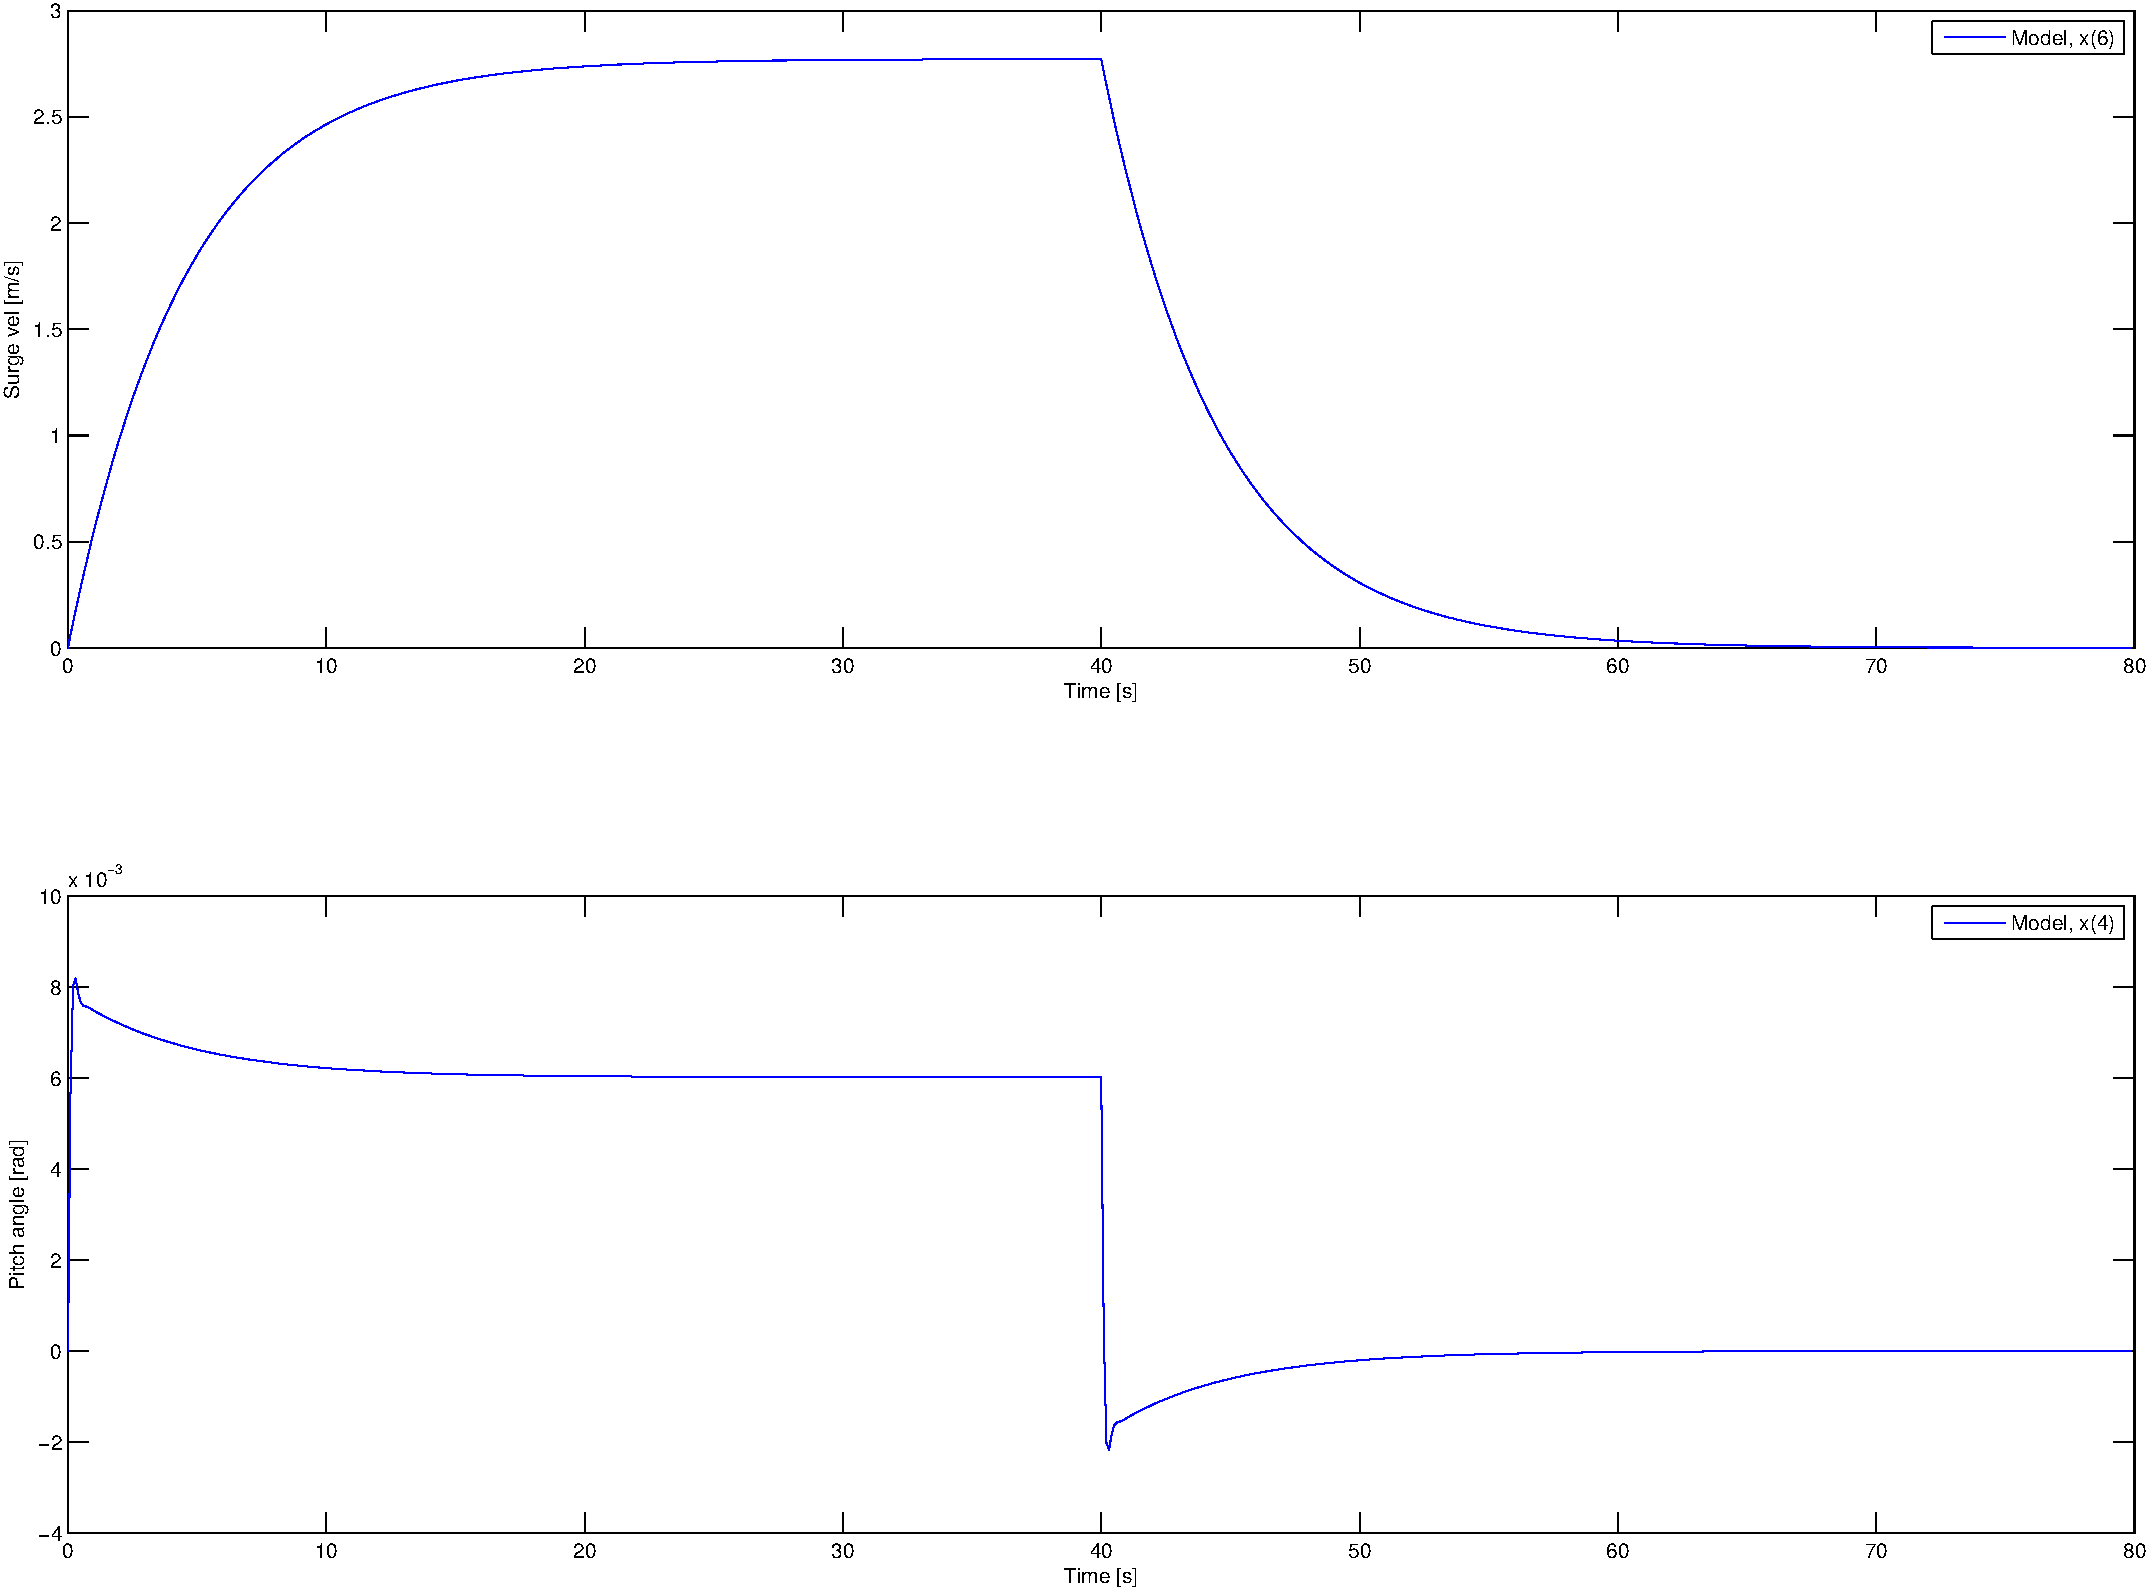
\includegraphics[width=0.8\textwidth]{fig/modelsurge}
  \caption{The output of the model in surge, where constant input is applied and after some time set to zero.}
  \label{fig:surgevel}
\end{figure}

\subsection{Stability}
A stability analysis can be conducted by examining the eigenvalues of the system. To ensure stability it is a criteria that the eigenvalues should all be stable for this system. This is fulfilled if the real part of all the eigenvalues of the system are negative, which implies a stable fixed point.

Stability of the discretised version also has to be checked by ensuring that the pole-zero map is within the unit circle. The eigenvalues of the Jacobian also needs to have absolute value less than one, which implies placement within the unit circle. If these are placed within the unit circle it is also a fixed point. If just one eigenvalue is greater than one it implies instability. If the eigenvalue is exactly equal to one it needs further investigation by looking more into the Jacobian.

\subsection{Simulation of the Model}
A final verification is to compare the correlation between a sea trail operated by human operator. It is desired to do multiple manoeuvers similar to what the system is supposed to perform. That is i.e. making a e.g. turning circle manoeuver and zig-zag manoeuvers.
\todo{Compare the simulation with the same inputs as a sea trail, especially for the inertial sensors}

\section{Kalman Filter design}
\label{sec:kfdesign}

\subsection{The \acl{KF}}

\nomenclature{$\boldsymbol\Phi$}{State transistion matrix of a discrete linear dynamic system}
\nomenclature{$\mathbf G$}{Input matrix}
\nomenclature{$\mathbf H$}{Measurement sensitivity matrix defining the linear relationship between the state of the dynamic system and the measurements that can be made}
\nomenclature{$\mathbf K$}{Kalman gain matrix}
\nomenclature{$\mathbf u$}{Input vector}
\nomenclature{$\mathbf x$}{State vector of a linear dynamic system}
\nomenclature{$\hat{\mathbf{x}}$}{Estimated state vector}
\nomenclature{$\mathbf{z}$}{Measurement vector}
\nomenclature{$\mathbf{w}$}{Process noise vector}
\nomenclature{$\mathbf{v}$}{Measurement noise vector}
\nomenclature{$\mathbf R$}{Covariance matrix of observational (measurement) uncertainty}
\nomenclature{$\mathbf P$}{Covariance matrix of state estimation uncertainty}
\nomenclature{$\mathbf Q$}{Covariance matrix of process noise in the system state dynamics}


A \ac{KF} is a type of observer that can be applied to estimate the state vector. This is done to filter the measurements from the vessel and smooth these. If the measurements are too noisy, such that the vessel changes direction suddenly, but should be surging forward, a filter can predict the modelled direction and compare this to the measurement.

The \ac{KF} comprises the deterministic part \todo{Deterministic part? nick} of the model which estimates the state vector. This is corrected by means of measurements to estimate the final state vector.

The \ac{KF} is drawn as a block diagram as seen on figure~\vref{fig:blockkf} illustrating both the process and the \ac{KF} together. The upper part represent the process, which can both be a simulated model or the real vessel with measurements, here it is a linear state space model. The lower part is the \ac{KF} which takes in the measurements and estimates the new state vector based on these measurements. The \ac{KF} can be of different types: \ac{LKF}, \ac{EKF} or \ac{UKF}. The figure illustrates the \ac{LKF}. Choosing between these types of filters depends on the type of model used and the application. 


\subsection{\acl{LKF}}
The process model is the usual state space model in discrete form as:
\begin{align}
x_k &= \Phi_{k-1} x_{k-1} + G u_{k-1} + w_{k-1}\\
z_k &= H_k x_k + v_k
\end{align}
\noindent The \ac{LKF} prediction and update can be written as:
\begin{itemize}\tightlist
\item Prediction
\begin{align}
\hat x_k^- &= \Phi_{k-1}\ \hat x_{k-1}^+ + G u_{k-1} \\
P_k^- &= \Phi_{k-1}P_{k-1}^- \Phi_{k-1}^\top + Q_{k-1}
\end{align}
\item Update
\begin{align}
\bar{\mathbf{z}}_k &= z_k - H_k\ \hat x_k^-\\
S_k &= H_k\ P_k^-H_k^\top + R_k\\
K_k &= P_k^-H_k^\top S_k^{-1}\\
\hat x_k^+ &= x_k^- + K_k \bar{\mathbf{z}}_k\\
P_k^+ &= (I - K_k H_k) P_k^-
\end{align}
\end{itemize}

\begin{figure}
	\centering
	\includesvg{kf_on_sys}
	\caption{Block diagram of a \acl{LKF} resulting in the state estimate $\hat x_k^+$.}
	\label{fig:blockkf}
\end{figure}

Where $P_{k}^-$ is the covariance propagation, $P_{k}^+$ is the update of covariance propagation, $Q$ is a covariance matrix with sensor variances and $R$ is a covariance matrix with model variances. $Q$ is a measure of how much the model is to be trusted. If the variance of the sensors are high this will imply that the model are to be trusted more than the noisy sensor measurements. These variances can sometimes be measured directly at the sensors and used in the $Q$ matrix. This leaves the $R$ matrix as the only design matrix left. $R$ is a measure of how much the measurement are to be trusted. If the variance of the model are high it might be better to trust the actual measurements. $z_k$ is the measurements from the sensors and $\bar{\mathbf{z}}_k$ is the difference between the measurements and the predicted state vector, $\hat x_k^-$. $S_k$ is the covariance matrix of the residual with the variance of the model included. $K_k$ is the optimal Kalman gain, in a \ac{MMSE} sense. 

\subsection{\acl{EKF}}
The above mentioned \ac{LKF} can only be applied on linear systems and transitions. Therefore is this not suited at the AAUSHIP. The position from the \ac{GPS} and the acceleration measurements needs to be rotated with a rotational matrix, which leads to non-linearities in the system. This can be seen on figure \vref{fig:intermediate-calc}. This entails that a \ac{LKF} cannot be used and an \ac{EKF} can be suited. The \ac{EKF} is used to linearise the non-linear terms in the system around the current estimate. In this case it will linearise the transition around the current measurements from the sensors to estimate the true output. The \ac{EKF} can be formulated in discrete form with the prediction and an update as:
\begin{itemize}\tightlist
\item Prediction
\begin{align}
\hat x_k^- &= f(\hat x_{k-1}^-,u_{k-1})\\
P_k^- &= F_{k-1}P_{k-1}^-F_{k-1}^\top+Q_{k-1}
\end{align}
\item Update
\begin{align}
\bar{\mathbf{z}}_k &= z_k - h(\hat x_k^-)\\
S_k &= H_k\ P_k^-H_k^\top + R_k\\
K_k &= P_k^-H_k^\top S_k^{-1}\\
\hat x_k^+ &= x_k^- + K_k \bar{\mathbf{z}}_k\\
P_k^+ &= (I - K_k H_k) P_k^-
\end{align}
\end{itemize}
where the state transition and observation matrices are defined by their respective jacobians:
\begin{align}
F_{k-1} &= \left.\frac{\partial f}{\partial x}\right|_{\hat x_{k-1}^-,u_{k-1}} \label{eq:EKFF}\\
H_k &= \left.\frac{\partial h}{\partial x}\right|_{\hat x_{k}^-}
\end{align}

\subsection{\acl{KF} in the case of AAUSHIP}
\label{sec:kfonaauship}
The input is given by the forces applied to the vessel. On AAUSHIP with the two twin propellers and two side thrusters as illustrated in section~\vref{sec:thrust_allocation}, this will result in forces in the surge and sway direction as well as a torque around yaw, the roll and pitch torques are neglected, such that the input vector $u_k$ becomes.
\begin{align}
u_k = \tau_k =
\begin{bmatrix}
X & Y & 0 & 0 & N
\end{bmatrix}^\top
\end{align}
These are the forces that can be applied by the thrusters mounted at the vessel. It should be noted that the pitch and roll are not set as input, since no thrusters can control these, and should be treated as model variations.

The discrete input matrix $\Gamma$ is a $17 \times 5$ matrix from the discretised $B$ matrix from equation~\vref{eq:ss}. \todo{Should we use $\Gamma$ for $G$ as in done in other sources (e.g. fossen), such that the input matrix is not confused with the restoring force matrix from fossen?}
The $\Gamma$ matrix takes the forces in $X$, $Y$ and $N$ as input, and neglects inputs in $\phi$ and $\theta$. The forces in $\phi$ and $\theta$ are outputs from the system that makes the vessel change in pitch and roll.

The discrete system $\boldsymbol \Phi$ is a $17 \times 17$ from the discretised $A$ matrix from equation~\vref{eq:ss}, but expanded to contain the full state vector calculations.

The dimensions of the different matrices used are checked as a type of sanity check and verify that the matrices are in correct size.

The covariance propagation matrix, the uncertainty of the estimated state, is given by:
\begin{align}
P_k^- &= F_k\ P_{k-1}^-F^\top + Q_k\\
\text{dim}(P_k^-) &= [17 \times 17]\cdot [17 \times 17]\cdot [17 \times 17]^\top + [17 \times 17]
\end{align}
The $Q$ is the variances of each of the states from the full state vector.

The posteriori error covariance matrix, the update, is given by:
\begin{align}
P_k^+ &= (I - K_k\ H_k)P_k^-\\
\text{dim}(P_k^+) &= ([17 \times 17] - [17 \times 7]\cdot [7 \times 17])\cdot [17 \times 17]
\end{align}
which is a measure of the estimated accuracy of the state estimate. Adding a middle calculation as the residual covariance:
\begin{align}
S_k &= H\ P\ H^\top + R\\
\text{dim}(S_k) &= [7 \times 17]\cdot [17 \times 17]\cdot [7 \times 17]^\top + [7 \times 7]
\end{align}
The $R$ is variances from the sensors, which makes it sensor noise terms.

The updated Kalman Gain:
\begin{align}
K_k &= P\ H^\top\ S^{-1}\\
\text{dim}(K_k) &= [17 \times 17]\cdot [7 \times 17]^\top\cdot [7 \times 7]^{-1}
\end{align}
witch is optimal in a \ac{MMSE} sense. %\todo{Hvorfor virkede denne ac ikke? Har fjernet den tidtil videre} - Hah, det var slet ikke den som var fejlen.

State vector
\begin{align}
\hat{\mathbf x}=
\begin{bmatrix}
N & E & x_b & y_b & \phi & \theta & \psi & u & v & p & q & r & \dot u & \dot v & \dot p & \dot q & \dot r
\end{bmatrix}^\top
\end{align}

Measurement vector
\begin{align}
\mathbf z=
\begin{bmatrix}
N & E & \psi & u & v & a_x & a_y
\end{bmatrix}^\top
\end{align}

Measurement matrix defining the relationship between the state of the dynamic system and the measurements
\begin{align}
H_k =
\begin{bmatrix}
1 & 0 & 0 & 0 & 0 & 0 & 0 & 0 & 0 & 0 & 0 & 0 & 0 & 0 & 0 & 0 & 0 \\
0 & 1 & 0 & 0 & 0 & 0 & 0 & 0 & 0 & 0 & 0 & 0 & 0 & 0 & 0 & 0 & 0 \\
0 & 0 & 0 & 0 & 0 & 0 & 1 & 0 & 0 & 0 & 0 & 0 & 0 & 0 & 0 & 0 & 0 \\
0 & 0 & 0 & 0 & 0 & 0 & 0 & 1 & 0 & 0 & 0 & 0 & 0 & 0 & 0 & 0 & 0 \\
0 & 0 & 0 & 0 & 0 & 0 & 0 & 0 & 1 & 0 & 0 & 0 & 0 & 0 & 0 & 0 & 0 \\
0 & 0 & 0 & 0 & 0 & 0 & 0 & 0 & 0 & 0 & 0 & 0 & 0 & 1 & 0 & 0 & 0 \\
0 & 0 & 0 & 0 & 0 & 0 & 0 & 0 & 0 & 0 & 0 & 0 & 0 & 0 & 1 & 0 & 0 
\end{bmatrix}
\end{align}

The covariance matrix of observational (measurement) uncertainty $R_k$ is assumed to be uncorrelated with the other states, such that the matrix only becomes the variances, with no covariance elements as:
\begin{align}
&R_k = \diag{\mathbf{v}} =\\ \nonumber
&\diag{^\text{GPS}\sigma_{N}^2,\ ^\text{GPS}\sigma_{E}^2,\ ^\text{GPS}\sigma_{\psi}^2,\ ^\text{GPS}\sigma_{u}^2,\ ^\text{GPS}\sigma_{v}^2,\ ^\text{gyro}\sigma_{a_x}^2,\ ^\text{gyro}\sigma_{a_y}^2}
\end{align}
These variances can be found by letting the AAUSHIP be in steady state. The sensor outputs are read while in steady state to check the variances from these. This will be the variances of the individual sensor measurements thus the variances of the particular measurements. The test finding these variances can be found in appendix \todo{lav appendix og ref til det her}.

The covariance matrix of process noise in the system state dynamics is $Q_k$ and is assumed to be the variances of each individual state:
\begin{align}
&Q_k = \diag{\mathbf{w}} = \\ \nonumber
&\diag{\sigma_{N}^2, \sigma_{E}^2, \sigma_{x_{b}}^2, \sigma_{y_{b}}^2, \sigma_{\phi}^2, \sigma_{\theta}^2, \sigma_{\psi}^2, \sigma_{u}^2, \sigma_{v}^2, \sigma_{p}^2, \sigma_{q}^2, \sigma_{r}^2, \sigma_{\dot u}^2, \sigma_{\dot v}^2, \sigma_{\dot p}^2, \sigma_{\dot q}^2, \sigma_{\dot r}^2}
\end{align} \todo{bedre notation for process og maalevarians?}
The variances can be found by making tests of the AAUSHIP. These should be carried out such that only one type of variance is tested at a time. By doing this, and testing around a known mean of the given state, makes it possible to test the variance of that particular state. The test finding these variances can be found in appendix \todo{lav appendix og ref til det her}.
\todo{What about $\mathbf w$ and $\mathbf v$? How to determine them correctly}

The $\mathbf F$, equation\ref{eq:EKFF} from the previous calculations, are the $[17 \times 17]$ system matrix, referred to as $\Phi$ in discrete case. This system matrix changes over time due the changes in the heading. The change of heading is not a linear transition which makes the system non-linear and therefore needs to be linearised about the given states of the system. Therefore this matrix is used as the system matrix in the \ac{EKF}, which is implemented in the AAUSHIP. $\Phi$ is designed to be
\begin{align}
\Phi = 
  \left[\begin{array}{c|ccc|c}
    I_{2\times 2} & 0_{2\times 5} & R_z (\psi) & 0_{2\times 3} & 0_{2\times 5}\\ \hline
    0_{10\times2}  & \multicolumn{3}{c}{\multirow{1}{*}{{$A_d$}}} \vline&  0_{10\times 5} \\ \hline
    0_{5\times 7} & & A_{d[6:10]} & & I_{5\times 5}
  \end{array}\right]
\end{align}
\todo{fix lower left corner alignment vline}


\chapter{Control}
\label{ch:control}
\head{This chapter describes the selected strategy from
	chapter~\vref{ch:selformctrl} in more detail, describing the exact
algorithm.}




% This is a summary of how they use Potential Fields in "UAV Formation Flight using 3D Potential Field"
\section{One Approach for Potential Fields}
In the following approach a potential field is generated for each
agent including obstacles, formation span, desired, and actual
position.  It will be a combination of virtual leader and potential
field. The principle generates a potential field to keep the formation
and that field is moved around as a virtual leader. When the virtual
leader is moved around it results in a deflection of the desired
position and causes the affected agents to get back into position. The
positions of the agents in the field is given individually to the
specific agents relative to the virtual leader. The approach generates
a single resulting vector for each agent which is used to guide the
agent. The potential field for each agent is generated from four
components:
\begin{align}
\tilde{F}_i^{tot} = F_{vl}+F_{ij}^{tot}+F_{ca}^{tot}+F_{oa}^{tot}
\end{align}
where:
\begin{ffk}
\firmlist%
\item[$F_{vl}$] virtual leader force
\item[$F_{ij}^{tot}$] inter-agent forces
\item[$F_{ca}^{tot}$] agent-agent collision avoidance forces
\item[$F_{oa}^{tot}$] agent-obstacle collision avoidance forces
\end{ffk}

\subsubsection{Virtual Leader, $F_{vl}$}
The virtual leader is an anchor of each formation, the \ac{FRP}, and
controls the movement of this. This movement can either be given as a
full trajectory of as a set of way points. The local virtual leader's
contribution to the field is defined as:
\begin{align}
F_{vl} &= K_{vl}(p_{vl}^n-p_i^n-[p_{vl}^n-p_{i0}^n])\\
&= K_{vl}(d_i-d_{i0})
\end{align}
$K_{vl}$ is a tuning parameter. $p_{vl}$ is position of the virtual
leader, $p_i$ is position of agent $i$, $p_{i0}$ is desired position
of agent $i$ and the $d$ is a shorter notation for the distances in
between. The virtual leader component guides the agents directly to
their desired positions relative to the virtual leader.

\subsubsection{Inter Vehicle Influence, $F_{ij}$}
This is the contribution of other vehicles to the potential field,
which is expressed as:
\begin{align}
F_{ij} &= K_{ij}(p_{j}^n-p_i^n-[p_{j0}^n-p_{i0}^n])\\
&= K_{ij}(d_{ij}-d_{ij0})
\end{align}
Similar to previously the $p$s are positions, $K_{ij}$ is a tuning
parameter and $d$ is a shorter notation for the distances in between.
This component preserves the formation by affecting the agents to keep
their respective desired distances among themselves. Hence the
weighting on each goal can be adjusted by $K_{vl}$ and $K_{ij}$ a
weighting that causes the agents to follow the virtual leader or to
preserve their desired formation.  In a swarm of $N$ agents the total
field for agent $i$ given by:
\begin{align}
F_{ij}^{tot} = \sum\limits_{j=1}^NF_{ij}(i,j) \text{ for } j\neq i
\end{align}

\subsubsection{Collision Avoidance, $F_{ca}$}
The collision avoidance takes effect when the agents get closer than a
pre defined distance of each other. It generates an additional field
component for the vehicle $i$ which points away from the entering
agent causing the agents to move away from each other. To ensure the
avoidance the component converges towards infinity in the centre of
the $i$'th agent. The $F_{ca}$ is expressed as:
\begin{align}
    F_{ca}^{ij}= 
\begin{cases}
		\left(
    \frac{K_{ca}r}{||d_{ij}||}-K_{ca}
		\right)
		\frac{\mathbf{d}_{ji}}{||\mathbf{d}_{ji}||}
		,& \text{for } ||d_{ij}||<r\\
    0,              & \text{otherwise}
\end{cases}
\end{align}
where $K_{ca}$ is a tuning parameter. $r$ is the safety radius for
collision and $d_{ij}$ is the distance between the individual agents.
The collision avoidance can be expressed in a total term of the
collision avoidance:
\begin{align}
F_{ca}^{tot} = \sum\limits_{j=1}^NF_{ca}^{ij} \text{ for } i\neq j
\end{align}

\subsubsection{Obstacle Avoidance, $F_{oa}$}
The same principle as for collision avoidance can be applied to
obstacle avoidance. Now each obstacle needs to be handled as an agent,
which will make the same result, but the reference is a little
different:
\todo{describe why the oa is different from the ca}
\begin{align}
    F_{oa}^{ik}= 
\begin{cases}
    \left( \frac{K_{oa}}{||d_{ki}||}-\frac{K_{oa}}{r}\right)
		\frac{\mathbf{d}_{{ki}}}{||\mathbf{d}_{ki}||},& \text{for } ||\mathbf{d}_{ki}||<r\\
    0,              & \text{otherwise}
\end{cases}
\end{align}
where $k$ denotes the counter for obstacles instead of other agents.
$K_{oa}$ is also a tuning parameter for the obstacle avoidance.
$d_{ki}$ is the vector between an agent and the obstacle, which in a
total term is summed up as:
\begin{align}
F_{oa}^{tot} = \sum\limits_{k=1}^MF_{oa}^{ik} \text{ for } i\neq k
\end{align}
Here $d_{ki}$ represents one of the $M$ place vectors which has the
effect of a detected obstacle.  The distance $r$ can be determined
dynamically depending on the velocity of the agent:
\begin{align}
r = r^{min} + K_r||\dot{p^n}||
\end{align}

\subsubsection{Potential field}
Now these forces was summed together to get
$\tilde{F}_i^{tot}$, that was just an intermediate vector, which needs
to be limited in a way, because this describes the speed the agents
can move with.

which gives the magnitude and direction of the
potential field for vehicle $i$ at its current position. As the
potential field does not need to expand to infinity it is reasonable
to define a maximum amplitude for the vector, while still keeping its
direction:
\todo{Denne afsluttende subsubsection er underligt formuleret, husk
det med tilden, og sikkert også hvordan vi jegner p\_r}
\begin{align}
	F_i^{tot} = \min\{\,\,\,||\tilde{F}_i^{tot}||\,\,\,,\,\,F_{max}\,\,\,\}\frac{\tilde{F}_i^{tot}}{||\tilde{F}_i^{tot}||}
\end{align}


\section{The Potential Field Strategy}
The theory of potential fields are implemented with the strategy
proposed in section \ref{sc:potential-fields}. The potential field is
generated for each individual agent at every update step to make the
formation move and converge to a specified formation and position. The
field is generated based on forces acting in a overlying potential
field structure where one force converges the agent to a desired
position, a force attracting the agent to obtain the desired formation
along the trajectory, a force repelling the agent from other agents if
their distance is too small and finally a force repelling the agents
from static objects. The latter two can seem the same, but the
repelling force will be larger for the agent-agent force due to the
fact that two agents could have course directly toward each other and
a more aggressive avoidance can be needed.

To be able to generate and simulate the potential field then
implementation needs to be generic. First it was developed with one
agent that needs to converge to a desired position and afterwards were
other agents added as obstacles and some static objects were added in
extend. From these obstacles it can be seen that a single agent is
able to converge to a position which makes it possible to expand such
that more agents can converge into formation with reference from
either a virtual leader or from each other. This will solve the
formation coordination task, where the following task will be the
group coordination task. The group coordination task has the goal to
move the formation around, which here will be done by making the
virtual leader, or an actual leader of the formation, follow a
specified trajectory. This will make the other agents follow this
leader and keep their formation on the trajectory.
\begin{figure}[htbp]
  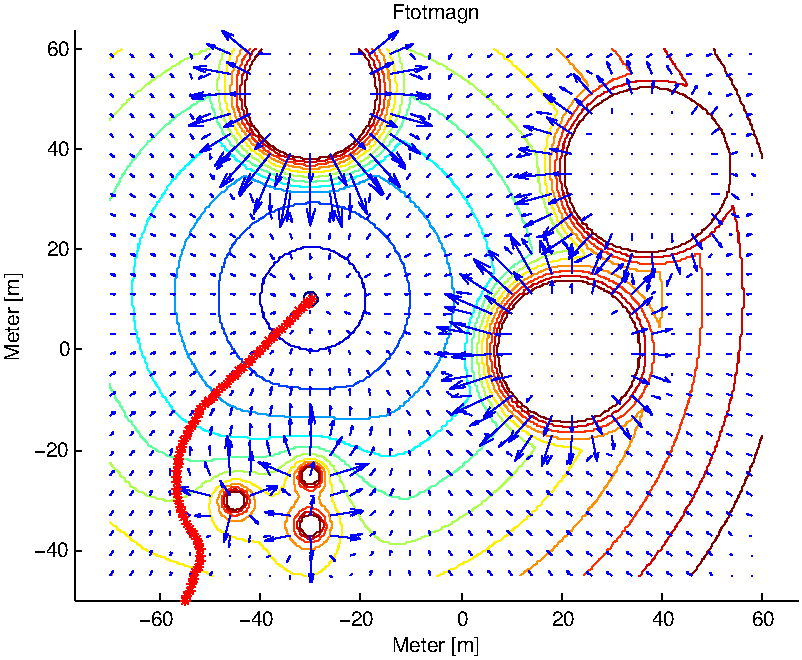
\includegraphics[width=0.9\textwidth]{fig/ftotmagnfigpdf1}
  \caption{Plot of one agent's trajectory with a desired position with obstacles to avoid}
  \label{fig:potfieldagenti}
\end{figure}
A plot for a total potential reference field for a single agent can be
seen on figure \ref{fig:potfieldagenti}. The red line made of crosses
is the trajectory that one single agent will follow, if the obstacles
to avoid in the plot are static. In the plot every object, either
another agent or an object, are kept static. So it shows how the
trajectory will be in one single time step. This will change in the
next time step if the other agents also move in the potential field.
The agent avoids obstacles on the way, where it can be seen that it
does not get into the safety radius of the obstacles. In this specific
plot is a safety radius ($r$) of $20$m chosen, such that the distance
from agent $p_i$ (The red trajectory) to any obstacle always will be
larger than $20$m.

The gains $K_{ca}$ and $K_{oa}$ are chosen equally to a constant as
240. If this gain is chosen smaller it will result in that the agents
are more allowed to approach the obstacles and get a little within the
radius, but then afterwards getting repelled from the object. It
corresponds to the gradient at the radius and how steep this is.

The same algorithm is applied where agent $i$ avoids other agents, agent $j$, $j+1$. This can be seen on figure \ref{fig:avoidagent}.
\begin{figure}[htbp]
  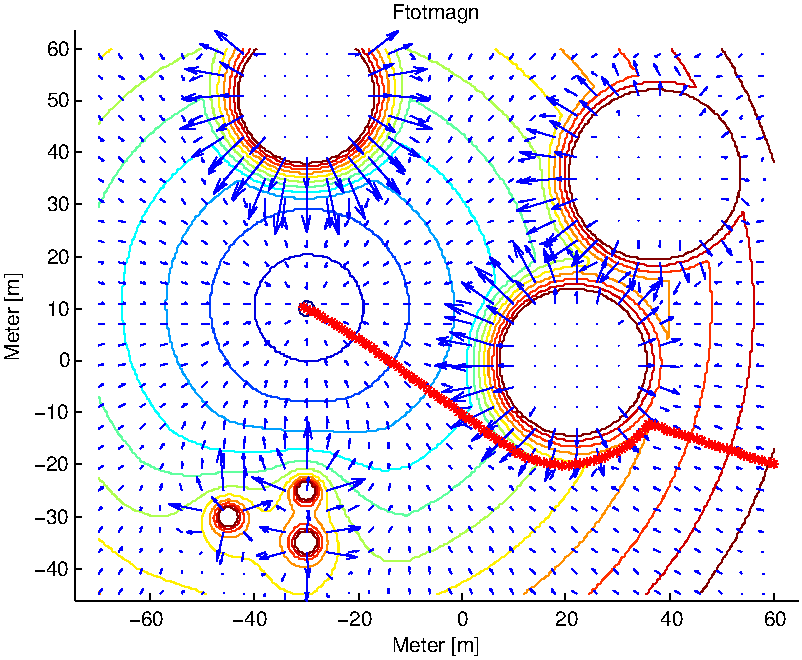
\includegraphics[width=0.9\textwidth]{fig/ftotmagnfigpdf}
  \caption{Agent $i$ avoids agent $j$ and converges to the minima at the virtual leader}
  \label{fig:avoidagent}
\end{figure}
Agent $i$ takes a direct course toward the virtual leader but meets
another agent as an obstacle. Agent $i$ moves on the boarder of agent
$j$ with the defined safety radius and afterwards diverges from agent
$j$ towards the virtual leader. This is all done by following the
lowest gradient at all times.

The gain of $K_{ij}$ is not to be interpret from figure
\ref{fig:potfieldagenti}. $K_{ij}$ is the gain to the force that
attracts the agents together by minimizing the distance in between
them. By doing this the agents will get faster into the desired
formation. The gain $K_{vl}$ does at some point the opposite. This
gain adjusts the weighting of how fixated the agents should be to
converge to the desired position. If this gain is relatively larger
than $K_{ij}$ then the agents will converge directly to their position
around the virtual leader and not converge to the desired formation on
the way. This implies that the scaling between $K_{vl}$ and $K_{ij}$
controls if the formation should converge to the desired formation on
the way to the desired position, or if agent $i$ should only have the
desired position in focus.

The grid in which the potential field is generated are limited with a
certain resolution while simulating the agents movement. This reduces
the directions of where the agents can move, which will not arise a
problem on the same level when implemented in reality. In the
simulation environment it reduces the resolution such that a single
field in the grid contains one value of magnitude of the potential
field, which makes the basis of a certain gradient to the field. The
agents are following the implementation of the steepest decent. This
generates a gradient towards the steepest decent, which the agent
tracks. The analogy can be seen as a bowl, or sphere in this case,
where a ball will converge towards the lowest point in the direction
of the minimum gradient.

The method of applying the grid with magnitude of the potential field
arises the problem with resolution, but also a problem that makes the
'corners' of the grid around the agent to be more likely to have the
steepest decent. This is seen as if the agent is placed in the middle
of a 3-by-3 matrix, and have eight placements around it. This problem
has been expanded with a solution such that a certain radius in the
potential field around an agent will be checked. The value at the
radius around the agent can be checked, and due to the equal distance
to every point, these will be weighted equally with respect to their
value. This makes in principle the possibility to make the agent go in
all directions which will be closer to the reality. When testing the
two methods against each other it is clear that the first proposed
with the grid structure did not have the same mobility thus not
preferable in simulations though it is simpler.
\todo{This section is not really clear}

Another problem that can become crucial arises when two agents or two
objects are within the radius of each other. This will result in a
local minima in the potential field between those objects. This will
create a small local minima in between these agents or objects. If an
agent converges toward this minima they cannot get out again. The
problem can be seen on figure \ref{fig:roevproblem}. The gains here
are chosen exactly the same as in figure \ref{fig:potfieldagenti}.
\begin{figure}[htbp]
  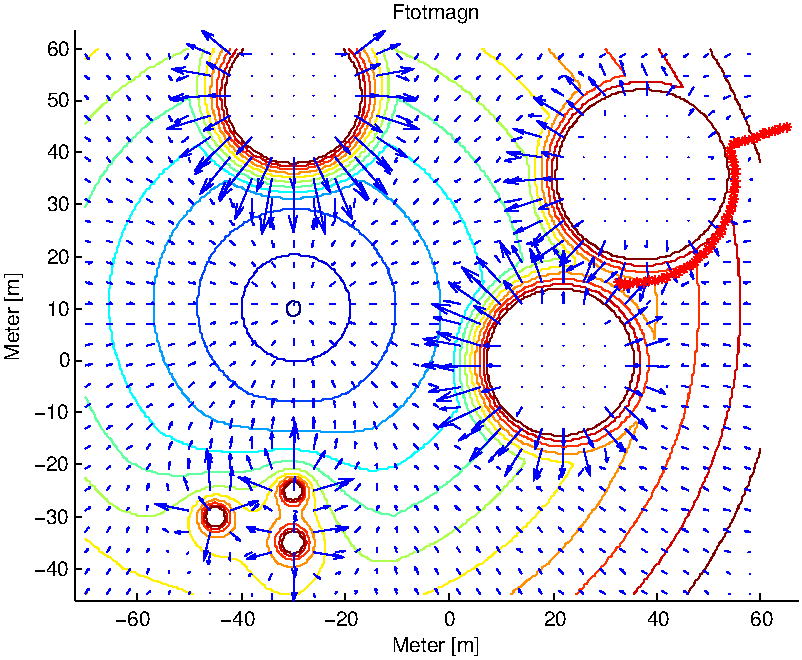
\includegraphics[width=0.9\textwidth]{fig/ftotmagnfigpdf3}
	\caption{An agent gets stuck due to a local minima between two other
	agents. The agent cannot get out of this minima unless the other two
	agents makes the space for the agent to pass through}
  \label{fig:roevproblem}
\end{figure}
The scenario on figure \ref{fig:roevproblem} has the following steps.
The agent $i$ moves in the direction of the steepest decent. Then it
gets to the border of another agent where it cannot go through thus
starts to go around this agent. The problem arises when agent $i$
reaches another agent on the way where it now has reached a local
minima. Now the steepest gradient will point at the position where the
agent already is thus making it think it has reached the end point.
Solutions to this problem can be formulated in different ways. One
solution could be to cluster the two objects together and instead of
making their potential field individually, then combine those together
and make an ellipsoid or even a circle formed obstacle of those
objects. This will ensure that the local minima disappears thus not
making an agent get stuck between those objects. Another solution is
to make an exception handler that can tell if agent $i$ has reached
the desired position. If it has not reached its end point, and the
position is constant on the same placement, it perturbs the desired
position of the agent until the direction of the steepest decent
changes more than a predefined value. This will mean that the agent is out of the local minima and can continue on the trajectory.
The solution of clustering the objects, that are too close, can be seen on figure \ref{fig:solroevproblem}.
\begin{figure}[htbp]
  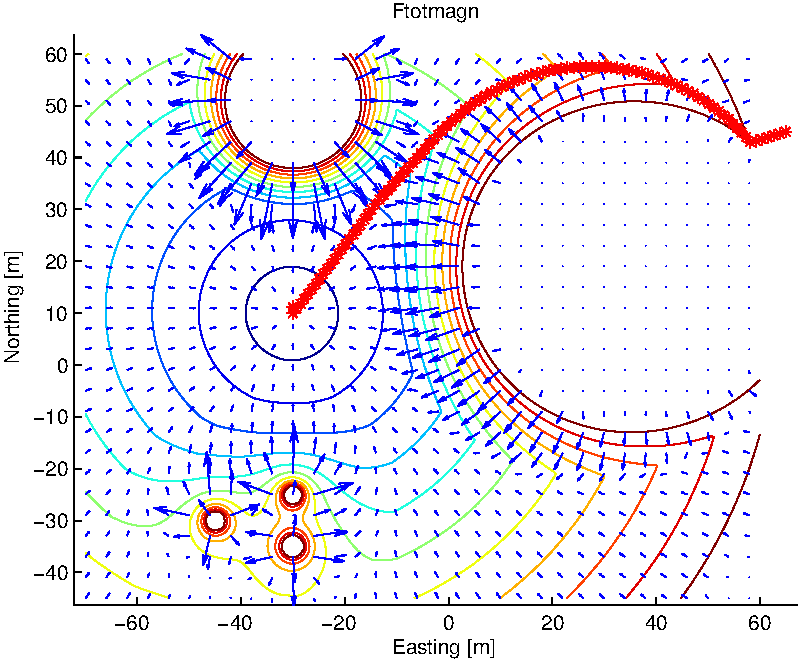
\includegraphics[width=0.9\textwidth]{fig/ftotmagnfigpdf4}
  \caption{An agent that before was stuck now does not get into a local minima close to the agents, as it now sees the two other agents as one larger agent.}
  \label{fig:solroevproblem}
\end{figure}
Here the first solution is applied where the two agetns, that were too close to each other, have been clustered into one, seen from the $i$'th agent. Now the local minima between the agents have been neglected and the $i$'th agent can generate its trajectory around the agents and continue to the endpoint of the potential field. The algorithm checks if the distances between the agents are lower that $2 \cdot r$. If this is the case it means that the $i$'th agent cannot generate a trajectory in between these agents, which can lead to a local minima. Therefore is the agents that are too close combined into one by generating the middle point between their positions and generating a new radius. This makes a larger circle where the two agents are in the subset. This cricle will be larger depending on the wanted safety radius thus rises the need to recheck the potential field again after have generated a new combined agent. If the radius of the new agent places it close to one of the single agents, these also might need to cluster. Thus the algorithm needs to run untill no distances between agents are $< 2 \cdot r$.
The algorithm generating this combined agent can be seen in pseudo code in algortihm \ref{al:clusteragents}.
\begin{algorithm}[H]
  \KwData{clustering of agents}
  initialization\;
  \If{$||\mathbf{p}_i , \mathbf{p}_j|| < 2 \cdot r$}{
  $\mathbf{p}_{j,new} \gets \text{mid point between}\ \mathbf{p}_i\ \text{and}\ \mathbf{p}_j$\\
  $r_{new} \gets \text{calc new r for}\ \mathbf{p}_{j,new}$\\
  delete $\mathbf{p}_i\ \text{and}\ \mathbf{p}_j \text{with}\ \mathbf{p}_{j,new}$
  }
  \caption{This pseudo code describes how agents that are too close to eachother are getting clustered and seen as one. The algorithm can also be applied for obstacles in the potential field.}
  \label{al:clusteragents}
\end{algorithm}
Firstly every distance between the agents are checked if it is lower than $2 \cdot r$. If the distance is lower, a new coordinate set needs to be calculated. The coordinates for the $\mathbf{p}_{j,new}$ is generated to the middle value of the two points
\begin{align}
\mathbf{p}_{j,new} = \frac{\mathbf{p}_i + \mathbf{p}_j}{2}
\end{align}
and afterwards can the new radius for $\mathbf{p}_{j,new}$ be found from
\begin{align}
r_{new} = \frac{||\mathbf{p}_i , \mathbf{p}_j||}{2} + r
\end{align}
The $r_{new}$ is visualized on figure \ref{fig:rnew}
\begin{figure}[htbp]
\centering
\includesvg{rnew}
\caption{Illustration of two agents close to each other clustering into one new agent. The two original agents, $i$ and $j$ are coloured in black and the new clustered object are coloured in green. The distance between $i$ and $j$ is coloured in red.}
\label{fig:rnew}
\end{figure}
This shows the relation between the normal safety radius and the new radius defined for the new clustered agent.

In the end this results in that the every agent needs a magnitude and
a direction of which they should move. This will be given depending on
the total environment where the agents are manoeuvring, and will be assigned by the gradient vector. When applying
this formation strategy a collision free movement is guaranteed which
is one of the more critical criteria to be fulfilled. \todo{Det her
skal der nok skrives lidt matematik om som viser det, eller en god
forklaring. Men dog er det jo en naturlig del af pot field.}


\subsection{Adding the Dynamics for Simulation}
\todo{Describe the block diagram connecting the potential field calculations,
an analogy to the wp\_gen script for the path follower.}

Describe the behaviour when a boat gets stuck in a local minima.

\begin{figure}[htbp]
\centering
\includesvg{potentialfield_block}
\caption{Block diagram showing the iteration process of using the
potential fields for computation of the input vector}
\label{fig:potentialfield_block}
\end{figure}

The potential field control system consists of multiple elements
as seen with the e flow is illustrated on the block diagram on
figure~\vref{fig:potentialfield_block}.

Part og this flow can be computed by the $i$'th ship themselves.

The implementation of this is tested in matlab, using the m-files;

potfield.m, pathgen.m, shipcontroller.m, simaauship.m

The simulation algorithm for the multiship potential field should keep
in mind that shall save the timeseries for the ship states, the
control inputs and the local reference trajectory for the $i$'th ship.

Ignoring the initialization of all the variables, the outer loop
guidance navigation and control algorithm using potential fields are
as follows.

The \ac{GNC} works by an array of mission specific way points given,
usually computed from a desired area used to create a lawnmower
pattern described in chapter~\vref{ch:pathgen} describing the path
generation.

\paragraph{Global Trajectory Generation}
Then different methods can be used to steer ships after this
trajectory. The simplest is the usual heading autopilot, which will
just steer the reading of the ship to the course angle to the
way point. Or more elaborate, ways is the use of the way points as
linesegments that the ship should follow. This is implemented with a
\ac{LOS} algorithm. This algorithm, can work, but it is too simple to
include obstacle or inter vehicle collisions. A way proposed to solve
this issue is to use the concept of potential fields.

\paragraph{Potential Field}
The potential field itself is merely some functions describing the
repulsive and repelling forces between points of interest in the map.
These points of interest are all objects that matters for the
navigation, that is all ships, the anchor point (virtual leader) of
the formation, and other point obstables. This using the methodology
described in the paper \citep{UAVff3dpf}.

The potential field is used in an iterative algorithm which can
calculate the direction (from the $i$'th boat to the desired position
spaned by a potential field defining the formation.

\paragraph{Local Trajectory Generation}
In the end, a reference path is calculated by the means of the
previous position and the result from the potential field
solver. It is calculated as the paper presents, \citep[eq.
48]{UAVff3dpf}.

\begin{align}
	\mathbf{p}_{i,r}^n = \mathbf{p}_i^n + \mathbf{F}_i ^\text{tot}
\end{align}

This is passed to the ships inner control loop.

When the trajectory is generated from a series of way points, which is
not ordered as a series of equidistant way points, it means that some
handling of when or how to update the position of the virtual leader
is needed.

For example; in the case, where the way points are far from each
other, it is still desired to make the virtual leader trajectory
converge the line between these two way points, kind of like the
\ac{LOS} guidance. Earlier a path following algorithm using a \ac{LOS}
principle was used, to calculate a course angle to a point projected
into the line between two way points with a specified lookahead
distance. The projection with the lookahead ensures convergence to the
line. But in the case of controlling the virtual leader, it is not
necessary to calculate the course angle from the virtual leader to the
projected point, because this is only a virtual anchor of the
formation, hence this only specifies where the geometry of the
formation is calculated from. 

For the inner loop, a heading based \ac{LOS} method can still be used,
but this should be calculated for every ship, with each their
reference position $\mathbf{p}_{i,r}$.

\begin{algorithm}[H]
	\KwData{track as global mission trajectory as way points}
	initialization\;
	\While{$m <=$ length of track}{
		\For{every $i$-th boat}{
			\If{formation is ok}{
				\If{$p_{vl}$ is inside the way point acceptance radius of the
				track}{
					$m \gets m + 1$\; 
					$p_{vl} \gets$ \textsl{LOS}$(\ p_{vl}\ ,\ $track($m$)\ )\;
				}
			}
			$(\ p_{d,i}\ ,\ F_{\text{tot},i}\ ) \gets $  \textsl{pathgen}(\ $p_i$\ ,\ $p0_i$\ )\;
			$p_{r,i} \gets p_i + F_{\text{tot},i}$\;
			$\psi_{d,i} \gets $ heading from $p_i$ to $p_d$\;
			$u_i \gets $ \textsl{controller}(\ $\psi_d$\ )\;
			\textsl{send input $u$ to ship}\;
			$x_i \gets $ \textsl{sense ship states}\;
			$p_i \gets $ position of $x_i$\; 
		}
	}
	\caption{This pseudo code describes how the potential field is used
	for each boat to calculate the reference for the inner controller
	for every boat at every time step. Every iteration in the while loop
	is a time step.\vspace{6pt}}
	\label{al:potfield}
\end{algorithm}

The algorithm~\vref{al:potfield} describes how the potential field
strategy can be simulated, were each iteration of the while loop is a
time step, which means that the control will continue until the
formation has reached the way point acceptance radius of the track.
This is to ensure that the formation anchor do not move forward if the
ships are not properly in formation. This is analogous with the group
coordination task as defined by \citep{thorvaldsen}, and described in
section~\ref{sc:initialisation}.

For the real implementation in \ac{ROS}'s node structure, only loop
inside the for every boat should be a node, such that there could be
$i$ instances of this node, each representing one boat. 




\todo{Describe how the dynamics will affect the trajectory.}

\chapter{\acs{ROS} design}
\head{This chapter describes the details of the implementation level,
which is done on a \acl{ROS} platform. This should provide all the
information needed to complete the implementation.}

It was decided to use \ac{ROS} in the implementation, It is used as an
other abstraction layer on top of the \ac{LLI}. In turn making AAUSHIP
modular and make it easy for others to write parts of the control
system without reimplementing basic components. This in turn makes it
an extensible platform, that should be easy to extend. \ac{ROS} is a
project available at \url{http://ros.org}, which describes itself in
short as following:

\begin{quote}
\textit{\noindent
	ROS (Robot Operating System) provides libraries and
	tools to help software developers create robot applications. It
	provides hardware abstraction, device drivers, libraries,
	visualizers, message-passing, package management, and more. ROS is
	licensed under an open source, BSD license.
}
		
	\hfill ROS.org
\end{quote}

\section{\acs{ROS} terminology}
To start working with \ac{ROS} it is important to use the terminology
used by \ac{ROS} to avoid confusion. Therefore these  will be stated
in this section.  The idea of \ac{ROS} is to make it easy to build a
system modularly, and this is achieved byt using almost
``self-contained'' code segments called \textit{nodes}, which is
application parts that is run as its own process. A node should be
designed to execute limited tasks such as image processing or similar
atomic processes. These nodes can then communicate with other nodes by
the means of two main communication forms called \textit{topics} and
\textit{services}.

\begin{description}
\item[The topic] is an asynchronous connection, that can \textit{publish}
from many nodes and be \textit{subscribed} by many nodes. This means
that it is a multicast form for providing data.
\item[The service] is a synchronous connection that is used between one node
to another node. This is only unicast.
\end{description}

An illustration of multiple nodes connected via topics and a service
is on figure~\vref{fig:ros-node-simple-concept}. This concept can also
be used across multiple machines. This is illustrated in
figure~\vref{fig:ros-node-master-concept}. On this a new type of unique
node is introduced, this is the \ac{ROS} master. This is a required
component for a ROS system to run. The masters only purpose is to make
the nodes connect together via the topics or services. There can only
be one master per \ac{ROS} system. This also enables multiple machines
to share topics, by connecting the master that runs on one machine. In
short the masters sole purpose is to make these connections. It is
illustrated by the dashed arrows. Each node says that it want to i.e.
publish or subscribe to a certain topic. To connect a node from one
machine to another, the environment variable \texttt{ROS\_MASTER\_URI}
has to be set to the host with the master running, and the
\texttt{/etc/hosts} file has to be set on all machines with the other
machines hostnames.

\begin{figure}[htbp]
	\centering
	\includesvg{ros_node_simple_concept}
	\caption{Basic principle of the node abstraction illustrating a
	service and two topics. The topology chosen here is only to illustrate
	the possibilities.}
	\label{fig:ros-node-simple-concept}
\end{figure}

When that is said, that is not the whole picture of the topology. In a
need to make this flexible \ac{ROS} has made it such that the nodes
can be started and stopped kind of ``runtime''. That is such that it is
possible to have different configurations of nodes to run in different
scenarios, i.e. in development with debugging nodes and virtual sensor
nodes versus in the real mission where no debugging nodes is used and
real sensor nodes that use real sensor data is used.

\begin{figure}[htbp]
	\centering
	\includesvg{ros_node_master_concept}
	\caption{Concept showing the ROS master together with the nodes,
	also illustrating the masters role with multiple machines. Dashed
	lines hows that the node will either subscribe or publish to the
	topic. This only happens initially when connecting to a topic. Gray
	area is two physical separate but networked machines.}
	\label{fig:ros-node-master-concept}
\end{figure}

\section{ROS on AAUSHIP}
\begin{figure}[htbp]
	\centering
	\includesvg{ros_aauship_teleop}
	\caption{ROS configuration on AAUSHIP for manual tele operation.}
	\label{fig:ros-aauship-teleop}
\end{figure}



\descpart{Conclusion}{%
The end of the project is the conclusion and perspective.}
\section{Simulation of the selected strategies}
\label{sc:simofstrat}
\head{This section contains simulations and verifications of the previously selected formation control strategies separated in steps from initial structure to complete formation control.}
\subsection{The potential field strategy}
The theory of potential fields are implemented with the strategy proposed in section \ref{sc:potential-fields}. The potential field is generated for each individual agent at every update step to make the formation move and converge to a specified formation and position. The field is generated based on forces acting in a overlying potential field structure where one force converges the agent to a desired position, a force attracting the agent to obtain the desired formation along the trajectory, a force repelling the agent from other agents is their distance is too small and finally a force repelling the agents from static objects. The latter two can seem the same, but the repelling force will be larger for the agent-agent force due to the fact that two agents could have course directly toward each other and a more aggressive avoidance can be needed.

To be able to generate and simulate the potential field then implementation needs to be generic. First it was developed with one agent that needs to converge to a desired position and afterwards were other agents added as obstacles and some static objects were added in extend. From these obstacles it can be seen that a single agent are able to converge to a position which makes it possible to expand such that more agents can converge into formation with reference from either a virtual leader or from each other. This will solve the formation coordination task, where the following task will be the group coordination task. The group coordination task has the goal to move the formation around, which here will be done by making the virtual leader, or an actual leader of the formation, follow a trajectory specified. This will make the other agents follow this leader and withhold their formation on the trajectory.
\begin{figure}[htbp]
  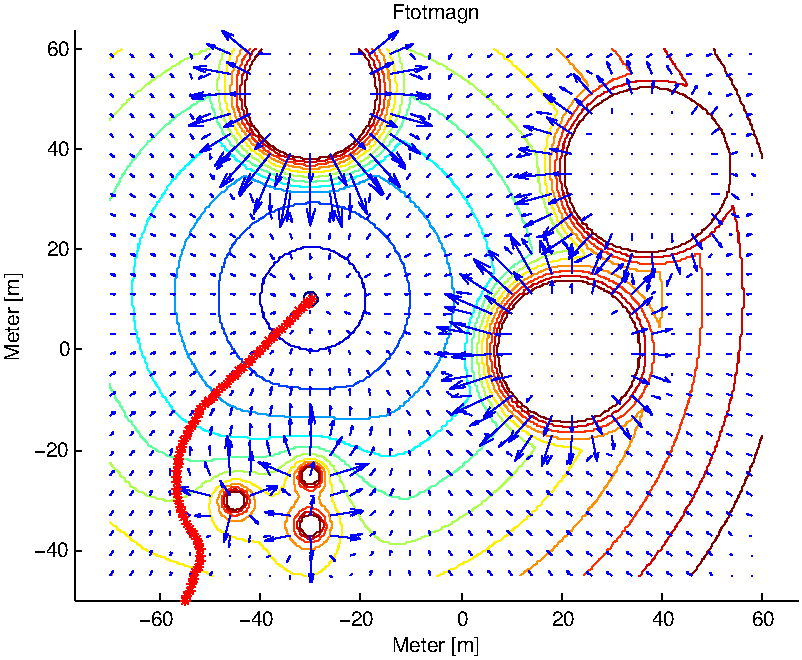
\includegraphics[width=0.9\textwidth]{fig/ftotmagnfigpdf1}
  \caption{Plot of one agent's trajectory with a desired position with obstacles to avoid}
  \label{fig:potfieldagenti}
\end{figure}
A plot for a total potential reference field for a single agent can be seen on figure \ref{fig:potfieldagenti}. The red line made of crosses are the trajectory that one single agent will follow, if the obstacles to avoid in the plot are static. In the plot every object, either an other agent or an object, are kept static. So it shows how the trajectory will be in one single time step. This will change in the next time step if the other agents also move in the potential field. The agent avoids obstacles on the way, where it can be seen that it does not get into the safety radius of the obstacles. In this specific plot is a safety radius ($r$) of $20$m chosen, such that the distance from agent $p_i$ (The red trajectory) to any obstacle always will be larger than $20$m.
This radius applies both to other agents seen in the following equation
\[
    F_{ca}^{ij}= 
\begin{cases}
    \frac{K_{ca}r}{||d_{ij}||}-K_{ca},& \text{for } ||d_{ij}||<r\\
    0,              & \text{otherwise}
\end{cases}
\]
and to obstacles seen in the following equation
\[
    F_{oa}^{ik}= 
\begin{cases}
    \frac{K_{oa}}{||d_{ki}||}-\frac{K_{oa}}{r},& \text{for } ||d_{ki}||<r\\
    0,              & \text{otherwise}
\end{cases}
\]
where the gains $K_{ca}$ and $K_{oa}$ are chosen equally to a constant as 240. If this gain is chosen smaller it will result in that the agents are more allowed to approach the obstacles and get a little within the radius, but then afterwards getting repelled from the object. It corresponds to the gradient at the radius and how steep this is.

The same algorithm is applied where agent $i$ avoids other agents, agent $j$, $j+1$. This can be seen on figure \ref{fig:avoidagent}.
\begin{figure}[htbp]
  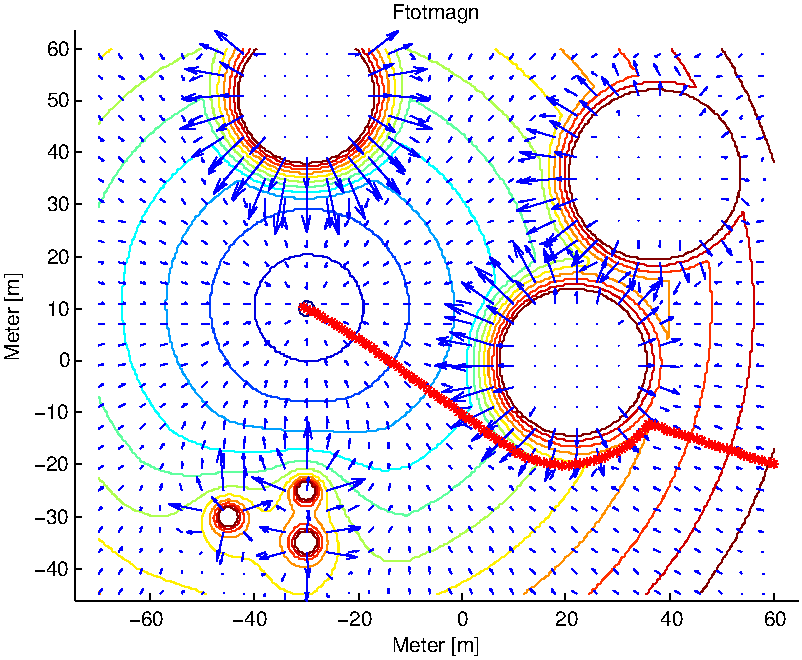
\includegraphics[width=0.9\textwidth]{fig/ftotmagnfigpdf}
  \caption{Agent $i$ avoids agent $j$ and converges to the minima at the virtual leader}
  \label{fig:avoidagent}
\end{figure}
Agent $i$ takes a direct course toward the virtual leader but meets another agent as an obstacle. Agent $i$ moves on the boarder of agent $j$ with the defined safety radius and afterwards diverges from agent $j$ towards the virtual leader. This is all done by following the lowest gradient at all times.

The gain of $K_{ij}$ is not to be interpret from figure \ref{fig:potfieldagenti}. $K_{ij}$ is the gain to the force that attracts the agents together by minimizing the distance in between them. By doing this the agents will get faster into the desired formation. The gain $K_{vl}$ does at some point the opposite. This gain adjusts the weighting of how fixated the agents should be to converge to the desired position. If this gain is relatively larger than $K_{ij}$ then the agents will converge directly to their position around the virtual leader and not converge to the desired formation on the way. This implies that the scaling between $K_{vl}$ and $K_{ij}$ controls if the formation should converge to the desired formation on the way to desired position, or if agent $i$ should only have the desired position in focus.

The grid in which the potential field is generated are limited with a certain resolution while simulating the agents movement. This reduces the directions of where the agents can move, which will not arise a problem on the same level when implemented in reality. In the simulation environment it reduces the resolution such that a single field in the grid contains one value of magnitude of the potential field, which makes the basis of a certain gradient to the field. The agents are following the implementation of the steepest decent. This generates a gradient towards the steepest decent, which the agent tracks. The analogy can be seen as a bowl, or sphere in this case, where a ball will converge towards the lowest point in the direction of the minimum gradient.

The method of applying the grid with magnitude of the potential field arises the problem with resolution, but also a problem that makes the 'corners' of the grid around the agent to be more likely to have the steepest decent. This is seen as if the agent is placed in the middle of a 3-by-3 matrix, and have eight placements around it. This problem has been expanded with a solution such that a certain radius in the potential field around an agent will be checked. The value at the radius around the agent can be checked, and due to the equal distance to every point, these will be weighted equally with respect to their value. This makes in principle the possibility to make the agent go in all directions which will be closer to the reality. When testing the two methods against each other it is clear that the first proposed with the grid structure did not have the same mobility thus not preferable in simulations though it is simpler.

Another problem that can become crucial arises when two agents or two objects are within the radius of each other. This will result in a local minima in the potential field between those objects. This will create a small local minima in between these agents or objects. If an agent converges toward this minima they cannot get out again. The problem can be seen on figure \ref{fig:roevproblem}. The gains here are chosen exactly the same as in figure \ref{fig:potfieldagenti}.
\begin{figure}[htbp]
  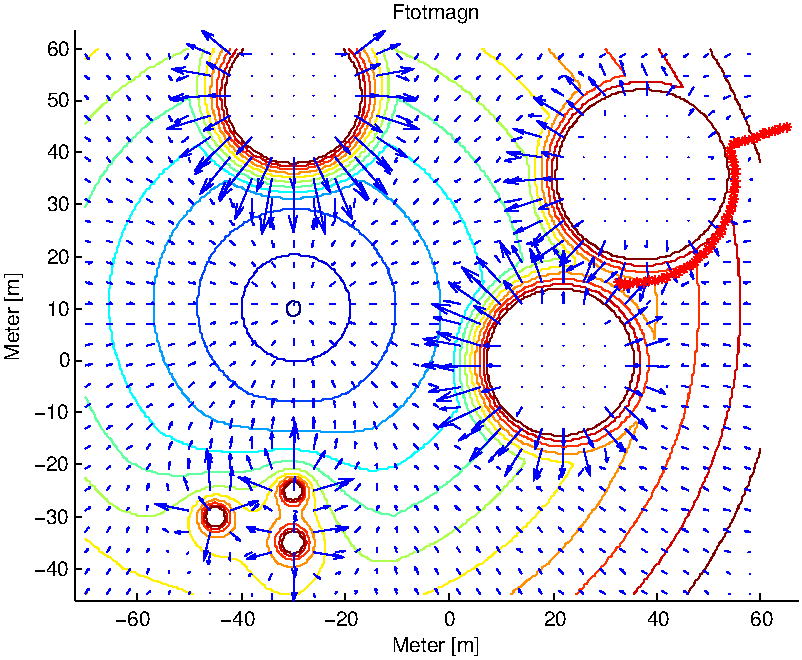
\includegraphics[width=0.9\textwidth]{fig/ftotmagnfigpdf3}
  \caption{An agent gets stuck due to a local minima between two other agents. The agent cannot get out of this minima unless the other two agents makes the space for the agent to pass through}
  \label{fig:roevproblem}
\end{figure}
The scenario on figure \ref{fig:roevproblem} has the following steps. The agent $i$ moves in the direction of the steepest decent. Then it gets to the border of another agent where it cannot go through thus starts to go around this agent. The problem arises when agent $i$ reaches another agent on the way where it now has reached a local minima. Now the steepest gradient will point at the position where the agent already is thus making it think it has reached the end point. Solutions to this problem can be formulated in different ways. One solution could be to cluster the two objects together and instead of making their potential field individually, then combine those together and make an ellipsoid or even a circle formed obstacle of those objects. This will ensure that the local minima disappears thus not making an agent get stuck between those objects. Another solution is to make an exception handler that can tell if agent $i$ has reached the desired position. If it has not reached its end point, and the position is placed in a constant spot, it perturbs the desired position of the agent until the direction of the steepest decent changes. This will mean that the agent is out of the local minima and can continue on the trajectory.

In the end this results in that the every agent needs a magnitude and a direction of which they should move. This will be given depending on the total environment where the agents are manoeuvring. When applying this formation strategy a collision free movement are guaranteed which is one of the more critical criteria to be fulfilled. \todo{Det her skal der nok skrives lidt matematik om som viser det, eller en god forklaring. Men dog er det jo en naturlig del af pot field.}

\subsection{Adding the Dynamics for Simulation}
\todo{Should this be moved to the potentialfield.tex?}
Describe the block diagram connecting the potential field calculations,
an analogy to the wp\_gen script for the path follower.

Describe how the dynamics will affect the trajectory.

Describe the behaviour when a boat gets stuck in a local minima. hhjj

\begin{figure}[htbp]
\centering
\includesvg{potentialfield_block}
\caption{Block diagram showing the iteration process of using the
potential fields for computation of the input vector}
\label{fig:potentialfield_block}
\end{figure}

The potential field control system consists of multiple elements
as seen with the e flow is illustrated on the block diagram on
figure~\vref{fig:potentialfield_block}.

Part og this flow can be computed by the $i$'th ship themselves.


The implementation of this is tested in matlab, using the m-files;

potfield.m, pathgen.m, shipcontroller.m, simaauship.m

The simulation algorithm for the multiship potential field should keep
in mind that shall save the timeseries for the ship states, the
control inputs and the local reference trajectory for the $i$'th ship.

Ignoring the initialization of all the variables, the outer loop
guidance navigation and control algorithm using potential fields are
as follows.

The \ac{GNC} works by an array of mission specific way points given,
usually computed from a desired area used to create a lawnmower
pattern described in chapter~\vref{ch:pathgen} describing the path
generation.

\paragraph{Global Trajectory Generation}
Then different methods can be used to steer ships after this
trajectory. The simplest is the usual heading autopilot, which will
just steer the reading of the ship to the course angle to the
way point. Or more elaborate, ways is the use of the way points as
linesegments that the ship should follow. This is implemented with a
\ac{LOS} algorithm. This algorithm, can work, but it is too simple to
include obstacle or inter vehicle collisions. A way proposed to solve
this issue is to use the concept of potential fields.

\paragraph{Potential Field}
The potential field itself is merely some functions describing the
repulsive and repelling forces between points of interest in the map.
These points of interest are all objects that matters for the
navigation, that is all ships, the anchor point (virtual leader) of
the formation, and other point obstables. This using the methodology
described in the paper \citep{UAVff3dpf}.

The potential field is used in an iterative algorithm which can
calculate the direction (from the $i$'th boat to the desired position
spaned by a potential field defining the formation.

\paragraph{Local Trajectory Generation}
In the end, a reference path is calculated by the means of the
previous previous position and the result from the potential field
solver. It is calculated as the paper presents, \citep[eq.
48]{UAVff3dpf}.

\begin{align}
	\mathbf{p}_{i,r}^n = \mathbf{p}_i^n + \mathbf{F}_i ^\text{tot}
\end{align}

This is passed to the ships inner control loop.


When the trajectory is generated from a series of way points, which is
not ordered as a series of equidistant way points, it means that some
handling of when or how to update the position of the virtual leader
is needed.

For example; in the case, where the way points are far from each
other, it is still desired to make the virtual leader trajectory
converge the line between these two way points, kind of like the
\ac{LOS} guidance. Earlier a path following algorithm using a \ac{LOS}
principle was used, to calculate a course angle to a point projected
into the line between two way points with a specified lookahead
distance. The projection with the lookahead ensures convergence to the
line. But in the case of controlling the virtual leader, it is not
necessary to calculate the course angle from the virtual leader to the
projected point, because this is only a virtual anchor of the
formation, hence this only specifies where the geometry of the
formation is calculated from. 

For the inner loop, a heading based \ac{LOS} method can still be used,
but this should be calculated for every ship, with each their
reference position $\mathbf{p}_{i,r}$.



% Acceptance test
% Conclusion
% Perspectives

\cleardoublepage\descpart{Appendix}{%
The appendix includes chapters which are important for the project, but not necessarily interesting to the reader of the report.}
\appendix
\chapter{Identification of hydrodynamic coefficients}
\label{app:damping}

\section{Purpose}
The purpose with this test is to
identify the hydrodynamic coefficients used in the linear model for
AAUSHIP, being the hydrodynamic damping coefficients for the 5 \ac{DOF} damping
matrix~\vref{eq:damping-matrix} and the restoring force during pitch and roll. This is accomplished by
three sea trails; a surge test, a sway test and a yaw
test, performed in a lake, and two tests to determine pitch and roll, performed in a small pool.

\section{Theory}
The surge, sway and yaw tests are performed with theory of one method of testing, and theory of another method is used when determining pitch and roll. The damping in surge, sway and yaw is estimated by fitting data to a first order differential equation where the pitch and roll dampings are determined from fitting onto a second order differential equation. These two ways of determining the damping coefficients will be denoted \textit{method one} for the first order fitting and \textit{method two} for the second order fitting.

\subsection{Which parameters to determine}
The parameters that needs to be determined is the damping coefficients
from the damping matrix. The 5 \ac{DOF} damping matrix is reduced from the 6 \ac{DOF} damping matrix from \ref{eq:6dofd}:
\begin{align}
D = -
\begin{bmatrix}
X_u & 0 & 0 & 0 & 0\\
0 & Y_v & Y_p & 0 & Y_r\\
0 & K_v & K_p & 0 & K_r\\
0 & 0 & 0 & M_q & 0\\
0 & N_v & N_p & 0 & N_r
\end{bmatrix}
\end{align}
and the coefficients from the restoring force matrix $G$, \ref{eq:restoreforce}, being:
\begin{align}
G = -
\begin{bmatrix}
0 & 0 & 0 & 0 & 0\\
0 & 0 & 0 & 0 & 0\\
0 & 0 & K_\varphi & 0 & 0\\
0 & 0 & 0 & M_\theta & 0\\
0 & 0 & 0 & 0 & 0
\end{bmatrix}
\end{align}
The different coefficients can be found by writing the complete dynamic system:
\begin{align}
M_{RB} \dot \nu + D\nu + G\eta = \tau
\end{align}
where:
\begin{align}
\nu =
\begin{bmatrix}
u & v & p & q & r
\end{bmatrix}^T
\quad , \quad
\eta =
\begin{bmatrix}
x & y & \varphi & \theta & \psi
\end{bmatrix}^T
\end{align}
and
\begin{align}
M_{RB} =
\begin{bmatrix}
m & 0 & 0 & mz_g & -my_g\\
0 & m & -mz_g & 0 & mx_g\\
0 & -mz_g & I_x & -I_{xy} & -I_{xz}\\
mz_g & 0 & -I_{yx} & I_y & -I_{yz}\\
-my_g & mx_g & -I_{zx} & -I_{zy} & I_z
\end{bmatrix}
\end{align}
The full 5 \ac{DOF} dynamic system equations can then be written as:
\begin{align}
M_{RB1}\dot \nu + D_{1} \nu &= \tau\\
M_{RB2}\dot \nu + D_{2} \nu &= \tau\\
M_{RB3}\dot \nu + D_{3} \nu + G_{3} \eta &= \tau\\
M_{RB4}\dot \nu + D_{4} \nu + G_{4} \eta &= \tau\\
M_{RB5}\dot \nu + D_{5} \nu &= \tau
\end{align}
%Which can be outlined as:
%\begin{align}
%\begin{bmatrix}
%m & 0 & 0 & mz_g & -my_g
%\end{bmatrix}
%\dot \nu &+
%\begin{bmatrix}
%X_u & 0 & 0 & 0 & 0
%\end{bmatrix}
%\nu = \tau\\
%\begin{bmatrix}
%0 & m & -mz_g & 0 & mx_g
%\end{bmatrix}
%\dot \nu &+
%\begin{bmatrix}
%0 & Y_v & Y_p & 0 & Y_r
%\end{bmatrix}
%\nu = \tau\\
%\begin{bmatrix}
%0 & -mz_g & I_x & -I_{xy} & -I_{xz}
%\end{bmatrix}
%\dot \nu &+
%\begin{bmatrix}
%0 & K_v & K_p & 0 & K_r
%\end{bmatrix}
%\nu = \tau\\
%\begin{bmatrix}
%mz_g & 0 & -I_{yx} & I_y & -I_{yz}
%\end{bmatrix}
%\dot \nu &+
%\begin{bmatrix}
%0 & 0 & 0 & M_q & 0
%\end{bmatrix}
%\nu = \tau\\
%\begin{bmatrix}
%-my_g & mx_g & -I_{zx} & -I_{zy} & I_z
%\end{bmatrix}
%\dot \nu &+
%\begin{bmatrix}
%0 & N_v & N_p & 0 & N_r
%\end{bmatrix}
%\nu = \tau
%\end{align}
The equations equal $\tau$, being the input to the vessel. Some of the contributions cannot have an input, since actuators for controlling pitch and roll is not implemented.

From the first row can the following be outlined:
\begin{align}
m\dot u - X_uu = \tau_{u}
\end{align}
From the second row can the following be outlined:
\begin{align}
m\dot v - Y_vv &= \tau_{v}\\
-mz_g\dot p - Y_pp &= 0\\
mx_g\dot r - Y_rr &= \tau_{r}
\end{align}
From the third row can the following be outlined:
\begin{align}
-mz_g\dot v - K_vv &= \tau_{v}\\
I_x\dot p - K_pp - K_\varphi\varphi &= 0\\
-I_{xy}\dot q &= 0\\
-I_{xz}\dot r - K_rr &= \tau_{r}
\end{align}
From the forth row can the following be outlined:
\begin{align}
mz_g\dot u &= \tau_{u}\\
-I_{yx}\dot p &= 0\\
I_y\dot q - M_qq - M_\theta \theta&= 0\\
-I_{yz}\dot r &= \tau_{r}
\end{align}
From the fifth row can the following be outlined:
\begin{align}
-my_g\dot u &= \tau_{u}\\
mx_g\dot v - N_vv &= \tau_{v}\\
-I_{zx}\dot p - N_pp &= 0\\
-I_{zy}\dot q &= 0\\
I_z\dot r - N_rr &= \tau_{r}
\end{align}
These equations can be utilized to calculate the coefficients from the damping matrix $D$ and the restoring force matrix $G$. The coefficients regarding surge, sway and yaw, $u$, $v$ and $r$, will be determined by \textit{method one} and coefficients regarding pitch and roll, $q$ and $p$, and the restoring force coefficients $K_\varphi$ amd $M_\theta$ will be determined by \textit{method two}.

\subsection{Method one}
\label{subsec:methodone}
This method is used to fit a first order differential equation to be able to estimate the damping coefficient. This is done by performing a test of the vessel. The vessel is accelerated from zero velocity to a constant velocity from where the input is taken away. This will make a velocity curve as seen on figure \ref{fig:phase3}.
\begin{figure}[htbp]
	\centering
	\includesvg[width=0.5\textwidth]{phase3}
	\caption{Constant velocity followed by zero input.}
	\label{fig:phase3}
\end{figure}
From this it is possible to fit the dynamic model including damping of the vessel such that the damping coefficient can be determined. When looking at the motion in surge, this should be fitted by the following method. The dynamic equation in surge, as a homogeneous equation, is given by:
\begin{align}
m \ddot x + D \dot x &= 0
\label{eq:dynsurgeeq}
\end{align}
A guess to fit such a first order differential equation could be:
\begin{align}
u = k \cdot \euler^{-st}
\end{align}
This is the expression of the surge speed, as seen from figure \ref{fig:phase3}. This is substituted into the dynamic equation to be able to fit the dynamic equation to the differential equation.
\begin{align}
m \dot u + Du &= 0\\
m \cdot (-ks\euler^{-st}) + D \cdot k \cdot \euler^{-st} &= 0\\
-ms+D&=0\\
s&=\frac{D}{m}
\end{align}
This makes the surge velocity to be expressed as:
\begin{align}
u = k \cdot \euler^{-\frac{D}{m}t}
\end{align}
By setting the time to zero gives the initial velocity:
\begin{align}
u_0 = k
\end{align}
After the damping is determined is the input force the only unknown in the dynamic equation \eqref{eq:dynsurgeeq}. The input force, to reach the constant velocity $u_0$, can be determined by the same principle but should be applied to a curve rising from zero velocity to the constant velocity. This would look as seen in figure \ref{fig:phase1}.
\begin{figure}[htbp]
	\centering
	\includesvg[width=0.5\textwidth]{phase1}
	\caption{Zero velocity followed by constant velocity.}
	\label{fig:phase1}
\end{figure}
The differential equation to fit this curve would be given by the inhomogeneous equation:
\begin{align}
u_{\text{inh}} &= u_0 - u_{\text{h}}\\
u &= u_0 - k \cdot \euler^{-st}
\end{align}
where the $s$ still would be given as:
\begin{align}
s = \frac{D}{m}
\end{align}
From this is the input force, to reach $u_0$, given from:
\begin{align}
m \dot u + Du &= \tau
\end{align}

\subsection{Method Two}
\label{subsec:methodtwo}
The second method is used to determine the coefficients $Y_r$, $K_r$,
$N_r$, $Y_p$, $K_p$, and $N_p$ for the pitch and
roll cross terms in the damping matrix \eqref{eq:damping-matrix} and the restoring forces from $G$ being $K_\varphi$ and $M_\theta$. In
these tests is the vessel put to a certain angle in pitch and roll and
hereafter released. This will make the vessel go back to the buoyant
steady state, as seen on figure~\vref{fig:harmonic-damping}. The
damping must be determined by fitting \eqref{eq:kestcoswt} to the
measured data, then this can be used to identify the coefficients for
the second order differential equation. The procedure is illustrated by
calculating it with the example of $K_p$ and $K_\varphi$.

The damping coefficient $K_p$ can be found from the dynamic equation
of roll by: \todo{Indtast (4.26)  et sted of referet til den herfra,
med hensyn til $-K_\varphi$.}
\begin{align}
I_x\dot p + K_pp + K_\varphi\varphi &= 0
\label{eq:solveddyneq}
\end{align}
$\varphi$ is angle position of the vessel. This is the position that needs to follow the damping as seen on figure~\vref{fig:harmonic-damping}. This can be fit to a second order differential equation. The position of the angle can be expressed as:
\begin{align}
\varphi = k\euler^{-\sigma t} \cdot \cos(\omega_d t)
\label{eq:kestcoswt}
\end{align}
This is an under damped system, which is described by a second order
homogeneous linear equation given by:
\begin{align}
a\ddot y + b\dot y + cy = 0
\end{align}
Which can be normalized with the coefficient of $a$, such that it takes the form:
\begin{align}
\ddot y + \frac{b}{a}\dot y + \frac{c}{a}y = 0
\label{eq:parameterized}
\end{align}
For an under damped system this can be seen as:
\begin{align}
\ddot y + b\dot y + cy = 0\\
\ddot y + 2\zeta \omega_0 \dot y + \omega_0^2 y = 0
\label{eq:normalized}
\end{align}
Where $\zeta$ is the exponential damping ratio of the system and $\omega_0$ is the undamped natural frequency. The solution to this is guessed as:
\begin{align}
y(t) = k\euler^{-st}
\label{eq:solutionguess}
\end{align}
This will make the curve as the damping from the pitch and roll dampings. Substituting this into \ref{eq:normalized}, and transforming, gives:
\begin{align}
s^2k\euler^{-st} + 2\zeta \omega_0sk\euler^{-st} + \omega_0^2k\euler^{-st} = 0
\end{align}
Which can be divided by $k\euler^{-st}$:
\begin{align}
s^2 + 2\zeta \omega_0s + \omega_0^2 = 0
\label{eq:dampeq}
\end{align}
The solution for the second order polynomial in \ref{eq:dampeq} is
then:
\begin{align}
s = \frac{-2\zeta \omega_0 \pm \sqrt{4\zeta^2\omega_0^2-4\omega_0^2}}{2}
\end{align}
where:
\begin{align}
a &= 1\\
b &= 2\zeta \omega_0\\
c &= \omega_0^2
\end{align}
Which for an under damped system can be expressed in the complex form:
\begin{align}
s \stackrel{\zeta < 1}{=} &-\zeta\omega_0\pm\omega_0\sqrt{1-\zeta^2}\\
= &-\sigma\pm j\omega_d
\end{align}
Where:
\begin{align}
\zeta\omega_0 &= \sigma\ \text{from equation} \ref{eq:kestcoswt}, \text{which is the real part}\\
\omega_0\sqrt{1-\zeta^2} &= \omega_d\ \text{from equation} \ref{eq:kestcoswt}, \text{which is the imaginary part}
\end{align}
By comparing \ref{eq:parameterized} and \ref{eq:dampeq} it can be seen that:
\begin{align}
a &= 1\\
b &= 2\zeta\omega_0 = \frac{K_p}{I_x}\\
c &= \omega_0^2 = \frac{K_\varphi}{I_x}
\end{align}
From the fitting of data is two variables known:
\begin{align}
\sigma &= \zeta\omega_0\\
\omega_d&=\omega_0\sqrt{1-\zeta^2}
\end{align}
This makes it possible to determine $K_p$ by:
\begin{align}
b &= 2\zeta\omega_0 = 2\sigma = \frac{K_p}{I_x}\\
K_p &= 2\sigma I_x
\end{align}
The coefficient $K_\varphi$ can be determined by: 
\begin{align}
\omega_d &= \omega_0\sqrt{1-\zeta^2}\\
\omega_d^2 &= \omega_0^2-(\zeta\omega_0)^2 = c - \sigma^2 = \frac{K_\varphi}{I_x}-\sigma^2\\
K_\varphi &= \omega_d^2I_x+\sigma^2I_x
\end{align}
This makes the dynamic equation with roll as:
\begin{align}
I_x\ddot \varphi + K_p\dot\varphi + K_\varphi\varphi &= 0\\
I_x\ddot \varphi + (2\sigma I_x)\dot \varphi + (\omega_d^2I_x+\sigma^2I_x)\varphi &= 0
\label{eq:solveddyneq}
\end{align}


%This can be rewritten by the following:
%\begin{align}
%-mZ_g\ddot \varphi + Y_p\dot \varphi - \tau_{hyd,hs} = 0\\
%as^2+bs+c=0
%\end{align}
%This makes, in the standard solution of the second order equation, $a=-mZ_g$, $b=Y_p$ and $c=-\tau_{hyd,hs}$. The standard solution will then become:
%\begin{align}
%s &= \frac{-b\pm\sqrt{b^2-4ac}}{2a}\\
%s &= \frac{-Y_p\pm\sqrt{Y_p^2-4(-mZ_g)\tau_{rest}}}{2(-mZ_g)}
%\end{align}
%This can then be fit to a position given by the previous:
%\begin{align}
%\varphi = k\euler^{\left(\frac{-Y_p\pm\sqrt{Y_p^2-4(-mZ_g)\tau_{rest}}}{2(-mZ_g)}\right)t} \cdot \cos(\omega t)
%\end{align}
%This makes a solution at zero degree, being the horizontal equilibrium, as:
%\begin{align}
%s\big|_{\varphi=0} = \frac{-Y_p}{-2mZ_g}
%\end{align}


\subsubsection{Surge test}
\begin{align}
m\dot u + X_uu = \tau_{u}
\end{align}
where only \textit{method one} is used.

\subsubsection{Sway test}
\begin{align}
m\dot v + Y_vv &= \tau_{v}\\
-mz_g\dot v + K_vv &= \tau_{v}\\
mx_g\dot v + N_vv &= \tau_{v}
\end{align}
where only \textit{method one} is used.

\subsubsection{Yaw test}
\begin{align}
mx_g\dot r + Y_rr &= \tau_{r}\\
-I_{xz}\dot r + K_rr &= \tau_{r}\\
I_z\dot r + N_rr &= \tau_{r}
\end{align}
where only \textit{method one} is used.

\subsubsection{Pitch test}
\begin{align}
I_y\dot q + M_qq + M_\theta \theta&= 0\\
\end{align}
where only \textit{method two} is used.

\subsubsection{Roll test}
\begin{align}
-mz_g\dot p + Y_pp &= 0\\
I_x\dot p + K_pp + K_\varphi\varphi &= 0\\
-I_{zx}\dot p + N_pp &= 0
\end{align}
where only \textit{method two} is used.

\section{Tools}
Tools needed are:
\begin{itemize}
	\item AAUSHIP equipped with:
		\begin{enumerate}
			\item Capability to set thrusters to equal setpoints and stop at
			the same time.
			\item Logging capability for \ac{IMU}, GPS1, GPS2 with UBX data
				and control inputs.
		\end{enumerate}
	\item Computer to set remote parameters and tele operation.
	\item RTK base station logging UBX data.
\end{itemize}
To be able to make the tests the AAUSHIP needs to have both forward thrusters and sideways thrusters. These are implemented and can be controlled from a computer.

\section{Method}
Two different types of measurements needs to be made. These are dependent on which coefficients that is wanted. The first type of test is split into three phases, as seen on figure \ref{fig:acceldecel}, and is approximated from a first order fitting. The second type of test is made as seen on figure \ref{fig:harmonic-damping}, and is approximated from a second order fitting.

In the first type of test is the vessel accelerated to constant velocity. When the constant velocity is ensured, the input force to the vessel is removed and zero input is therefore applied. This will correspond to a model like:
\begin{align}
M_{RB} \dot \nu_r + D\nu_r = 0
\label{eq:decelmodel}
\end{align}
An acceleration, constant velocity and deceleration will look like figure \ref{fig:acceldecel}.
\begin{figure}[htbp]
	\centering
	\includesvg[width=0.5\textwidth]{acceldecel}
	\caption{An acceleration followed by constant velocity followed by zero input.}
	\label{fig:acceldecel}
\end{figure}
\begin{figure}[htbp]
	\centering
	\includesvg[width=0.5\textwidth]{harmonic_damping}
	\caption{Pitch and roll response.}
	\label{fig:harmonic-damping}
\end{figure}
This makes it possible to determine some of the coefficients of the $D$ matrix. e.g. is the damping in the x direction determined by:
\begin{align} 
M_{11} \ddot x + D_{11} \dot x = 0
\label{eq:noinput}
\end{align}
The mass of the vessel can be measured, being the $M_{11}$. The velocity and acceleration can be estimated from measurements of the positions measured by the \ac{GPS} at the vessel. This makes the damping coefficient $D_{11}$ the only unknown in equation \ref{eq:noinput}. From this a linearisation can be made, see appendix \ref{app:damping}. From this can the damping coefficient be determined.

This makes it possible to determine the input force by applying a step input on the motors and let the vessel accelerate to the same constant velocity. This can be done since, due to the previous test, only the input is unknown. A model of this will look like:
\begin{align} 
M_{11} \ddot x + D_{11} \dot x = \tau
\label{eq:maxinput}
\end{align}
From this it is possible to estimate the input force as a linearisation, since this is the only unknown from equation \ref{eq:maxinput}.

This type of procedure is used in all of the first types of tests and can be put into steps.
\begin{enumerate}
	\item Step one is to apply force in one direction until a constant velocity is achieved and then measure the damping while the vessel is decelerating to estimate the damping coefficient.
	\item Step two can be made after knowing the damping coefficient. Then is only the input unknown and a step can be applied to accelerate the vessel to constant velocity again. From this step input can a input force be estimated.
\end{enumerate}

The second type of test is used when determining coefficients as pitch and roll, $r$ and $p$. In these tests is the vessel put to a certain angle in pitch or roll and is afterwards released. This will make the vessel converge to steady state, as seen on figure \ref{fig:harmonic-damping}. This is due to the acting restoring force due to that the vessel is perturbed away from its equilibrium and converges back to it. The convergence is dependent on the angle of either pitch or roll of the vessel, and therefore the tests need to be made from the same angle every time.

% When determining the forces in sway due to rolling, $Y_p$, the following equation needs to be outlined:
% \begin{align}
% M_{RB} \dot \nu + D \nu = \tau
% \end{align}
% which for roll will be:
% \begin{align}
% M_{RB2} \dot \nu =
% \begin{bmatrix}
% 0 & m & -mz_g & 0 & mx_g
% \end{bmatrix}
% \dot \nu
% \label{eq:rollmedmere1}
% \end{align}
% and
% \begin{align}
% D_2 \nu =
% \begin{bmatrix}
% 0 & Y_v & Y_p & 0 & Y_r
% \end{bmatrix}
% \nu
% \label{eq:rollmedmere2}
% \end{align}
% Since the roll is uncontrollable should the equation equal zero, due to no input. When taking the parts from equation \ref{eq:rollmedmere1} and \ref{eq:rollmedmere2} that consider only roll, and with no input, it reduces to the following equation:
% \begin{align}
% -mz_g \dot p + Y_pp = 0
% \end{align}
% This can be approximated to a second order equation fulfilling the convergence as shown on figure \ref{fig:harmonic-damping}. From this it is possible to determine the damping in roll due to a acting force in sway, $Y_r$.
% \todo{omkring her skal der rettes videre}

One of the important things are to decouple the tests such that the damping coefficients can be measured. This can, as a start, be performed in x-, y- and z-directions. The mixed damping coefficients, as the $Y_r$ (the force in y-direction due to a rotation), has got many components as shown above. But, after have performed the previous tests, these will become the next unknowns to be determined. Looking at the system as a 5 \ac{DOF} will make it possible to determine the coefficients needed. Some of the coefficients can be found from measurements made by \citep{13gr931}. The decoupled coefficients are tested from the equations in \ref{eq:syseq}.
\begin{subequations}
\begin{align}
M_{11} \ddot x + D_{11} \dot x = \tau\\
M_{22} \ddot y + M_{23} \ddot \psi + D_{22} \dot y + D_{23} \dot \psi = \tau\\
M_{45} \ddot y + M_{55} \ddot \psi + D_{45} \dot y + D_{55} \dot \psi = \tau
\end{align}
\end{subequations}
being
\begin{subequations}
\begin{align}
m \ddot x - X_u \dot x = \tau\\
m \ddot y + mx_g\ddot\psi - Y_v \dot y - Y_r \dot \psi = \tau\\
mx_g \ddot y + I_z\ddot \psi - N_v \dot y - N_r \dot \psi = \tau
\end{align}
\label{eq:syseq}
\end{subequations}

The tests performed are as follows:
\begin{enumerate}
	\item The first test is a \textit{surge} test. This test is done to test the forward damping coefficient being $X_u$ from the damping matrix $D$. The vessel will accelerate to a certain velocity and keep this. Then all input is put to zero and the vessel will decelerate. This will, as described in section \ref{sec:hydrocoeff}, give a damping coefficient in the forward motion. This is expressed as $m \ddot x - X_u \dot x = 0$ and $X_u$ can be estimated. A step input is now set on the vessel to see the acceleration from zero velocity to the same constant velocity as before. This now gives the input force at the vessel, which is the last unknown in $m \ddot x - X_u \dot x = \tau$. Both $X_u$ and $\tau$ is estimated by fitting to a first order differential curve, as described in \ref{subsec:methodone}. To make this test and data fitting is only position data in the forward motion from the \ac{GPS} of importance. The position can be differentiated twice, to give both velocity and acceleration of the vessel and cab be used to fit the acceleration and deceleration of the vessel.
	\item The second test is a purely \textit{sway} test. The vessel will make use of the sideways thrusters to move strictly sideways. This implies that there is no rotation or movement in $\psi$ and $x$. Thus makes the moving equation as $m \ddot y - Y_v \dot y = 0$. Here is the vessel again accelerated to a constant velocity and the input is then set to zero, and $Y_v$ can be determined. After this the sideways thrusters can be used to accelerate the vessel to the same constant velocity and the input can be estimated by $m \ddot y - Y_v \dot y = \tau$ where $\tau$ is the only unknown. $K_v$ and $N_v$ can be determined from the same test, though the fitting needs to be changed due to the new parameter from $M_{RB}$. The fitting should be done to the same type, namely like procedure \textit{method one} in \ref{subsec:methodone}. To make this test and data fitting is only position data in sideways motion from the \ac{GPS} of importance. This can be differentiated twice to give both velocity and acceleration in the sideways direction. This can be fitted to a acceleration and deceleration of the vessel when only moving in the sideways direction.
	\item The last test to perform is the \textit{yaw} test. In this test it is of importance to control the sideways thrusters such that the vessel will keep the position at both $x$ and $y$, such that only rotation is used to move the surrounding water. The vessel is accelerated to a constant angular velocity and the input is then set to zero. The damping of this will determine $N_r$ from $I_z\ddot \psi - N_r \dot \psi = 0$. Now the vessel needs to reach the constant angular velocity again from zero, and the input can now be estimated from $I_z\ddot \psi - N_r \dot \psi = \tau$. $Y_r$ and and $K_r$ can be determined from the same test, but the fitting is a little different due to the new parameter from $M_{RB}$. These fittings should be done as procedure \textit{method one} in \ref{subsec:methodone}. To make these should the position from the \ac{GPS} be measured to ensure that the vessel does not move of greater importance in forward and sideways directions. Measurements from the magnetometer and accelerometer is used to determine the heading and thereby the change on heading and the acceleration. The accelerometer is used to compensate the pitch and roll in the magnetometer measurements.
\end{enumerate}
The parameters in pitch and roll is determined by fitting data to \textit{method two} as described in \ref{subsec:methodtwo}. Previous work done by \citep{13gr931} has provided the data to be fitted. These data can be found on the cd, \todo{ref til cd}. The data is dependent of the position on the angle of the vessel and the equations is therefore formulated to fit these measurements. The fitting of the data is done as procedure \textit{method two} and no further tests needs to be performed. The tests shows pitch and roll, measured in a vicon motion tracking lab. The vessel is put to a maximum angle without level it into the water. Afterwards it is released and the vessel will damp to zero angle, being horizontal in steady water. To verify the data from \citep{13gr931} accelerometer will be collected both in pitch and roll from two simpler tests without the vicon motion tracking lab.

\section{Results}
\subsubsection{Surge test}
\missingfigure{Maalinger af acceleration fra 0 til konstant hastighed
+ Maaling af deceleration med 0 input fra konstant hastighed +
regræssionskurve af disse}
\subsubsection{Sway test}
While performing tests with sway it was rather difficult to get any reliable data from measurements. Weather conditions was almost perfect but there was a slight wind. This seemed from measurements to be enough to counteract the forces added by the bow thrusters. The vessel was not moving much over time, thus the measurements seems unreliable. Therefore is the parameters from sway approximated from observations of how fast the vessel was moving over time. The constants which needs to be approximated manually is $Y_\nu$, $K_\nu$ and $N_\nu$.

it is assumed, from observations, that the vessel moves in sway with a constant velocity being $0.1\frac{m}{s}$. From this velocity it is estimated that the vessel was on hold after 1 second. This gives the following damping:
\missingfigure{Maalinger af acceleration fra 0 til konstant hastighed
+ Maaling af deceleration med 0 input fra konstant hastighed +
regræssionskurve af disse}
\subsubsection{Yaw test}
\missingfigure{Maalinger af acceleration fra 0 til konstant vinkel
hastighed + Maaling af deceleration med 0 input fra konstant vinkel
hastighed + regræssionskurve af disse}

\newpage
\subsubsection{Pitch test}
\begin{figure}[H]
	\centering
	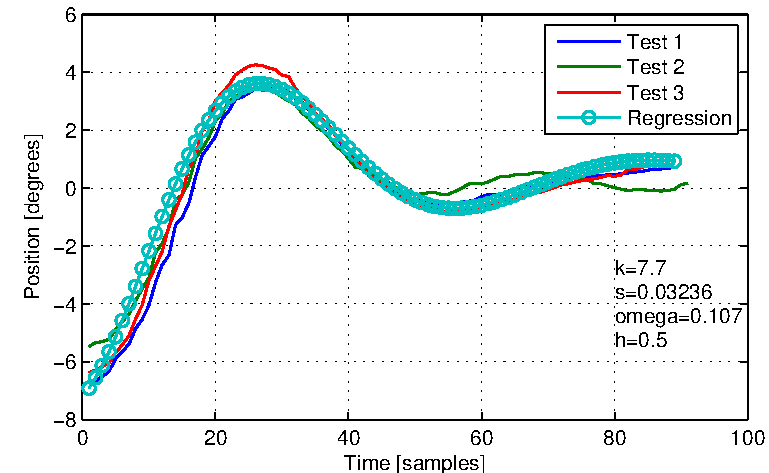
\includegraphics{plot/pbtest}
	\caption{Pitch test with Vicon, Bow pushed down.}
	\label{fig:pbtest}
\end{figure}
\begin{figure}[H]
	\centering
	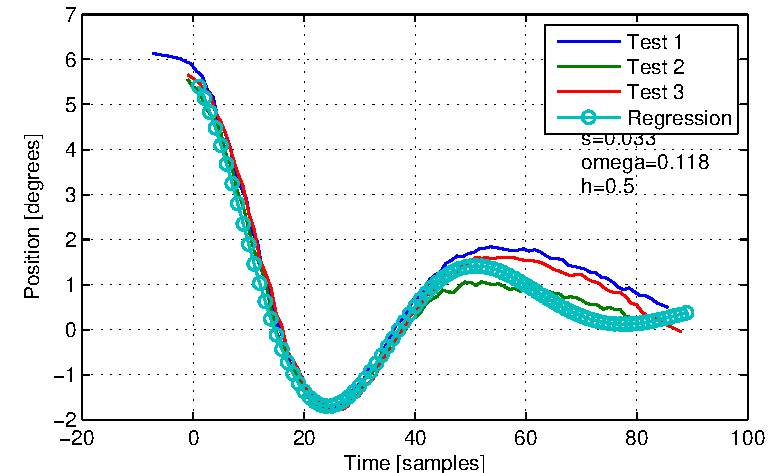
\includegraphics{plot/pstest}
	\caption{Pitch test with Vicon, Stern pushed down.}
	\label{fig:pstest}
\end{figure}

\newpage
\subsubsection{Roll test}
\begin{figure}[H]
	\centering
	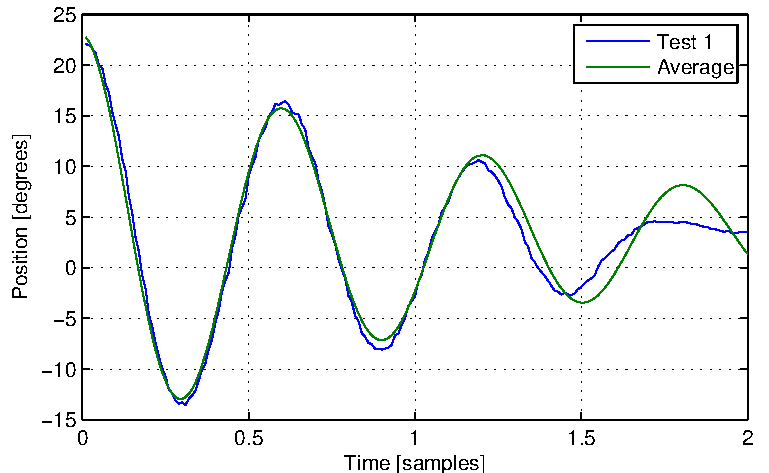
\includegraphics{plot/rltest}
	\caption{Roll left test with Vicon, Port side pushed down.}
	\label{fig:rltest}
\end{figure}
\begin{figure}[H]
	\centering
	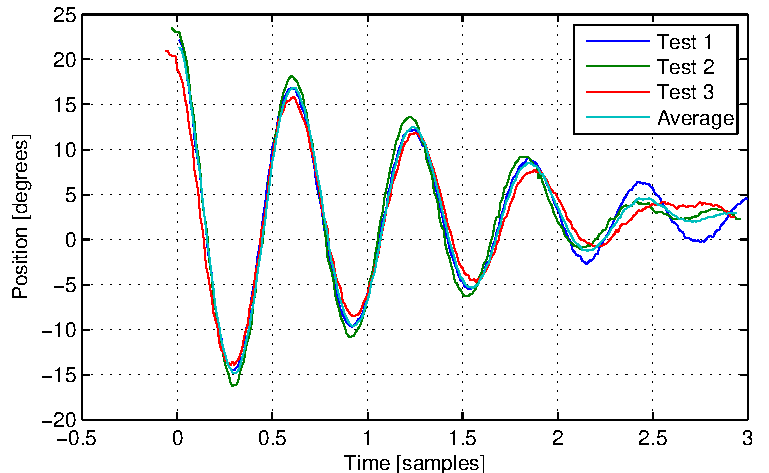
\includegraphics{plot/rrtest}
	\caption{Roll right test with Vicon, Starboard side pushed down.}
	\label{fig:rrtest}
\end{figure}


The rigid body constants for the vessel can be found in table \ref{tab:constants} and the results from measurements and estimation can be found in table \ref{tab:dmatrix}.
\todo{Disse skal måles op og sættes ind}
\begin{table}[htbp]
\centering
\begin{tabular}{ccc}
	\toprule
  Coefficient & Value \\
  \midrule
  $m$ & 13 \\
  $x_g$ & 0.03 \\
  $y_g$ & 0\\
  $z_g$ & 0.03\\
  $I_{xz}$ & -0.05359 \\
  $I_{zx}$ & -0.05359 \\
  $I_{xy}$ & -0.01260 \\
  $I_{yx}$ & -0.01260 \\
  $I_{yz}$ & -0.00108 \\
  $I_{zy}$ & -0.00108 \\
  $I_z$ & 1.10675 \\
  $I_y$ & 1.08921 \\
  $I_x$ & 0.06541 \\
  \bottomrule
\end{tabular}
\caption{Rigid body mass matrix constants for $M_{RB}$}
\label{tab:constants}
\end{table}

\begin{table}[htbp]
\centering
\begin{tabular}{ccc}
	\toprule
  Hydrodynamic\\Coefficient & Value \\
  \midrule
  $X_u$ & 2.86 \\
  $Y_v$ & 32.5 \\
  $K_v$ & -0.975 \\
  $N_v$ & 0.975 \\
  $N_r$ & 0.26285 \\
  $Y_r$ & 0.09263 \\
  $K_r$ & 0.01273 \\
  $Y_p$ & -0.00503 \\
  $K_p$ & 0.00084 \\
  $N_p$ & -0.00069 \\
  $M_q$ & 0.0712 \\
	\bottomrule
\end{tabular}
\caption{Results of fitted values and the calculated coefficients.}
\label{tab:dmatrix}
\end{table}

\begin{table}[htbp]
\centering
\begin{tabular}{ccc}
	\toprule
  Restoring force\\Coefficient & Value \\
  \midrule
  $K_\varphi$ & 0.0007 \\
  $M_\theta$ & 0.0150 \\
  	\bottomrule
\end{tabular}
\caption{Results of fitted values and the calculated coefficients.}
\label{tab:gmatrix}
\end{table}

This makes the linear damping matrix as:
\begin{align}
D = -
\begin{bmatrix}
2.86 & 0 & 0 & 0 & 0\\
0 & 32.5 & -0.00503 & 0 & 0.09263\\
0 & -0.975 & 0.00084 & 0 & 0.01273\\
0 & 0 & 0 & 0.0712 & 0\\
0 & 0.975 & -0.00069 & 0 & 0.26285
\end{bmatrix}
\end{align}
and the restoring for matrix as:
\begin{align}
G = -
\begin{bmatrix}
0 & 0 & 0 & 0 & 0\\
0 & 0 & 0 & 0 & 0\\
0 & 0 & 0.0007 & 0 & 0\\
0 & 0 & 0 & 0.0150 & 0\\
0 & 0 & 0 & 0 & 0
\end{bmatrix}
\end{align}
and the rigid body matrix as:
\begin{align}
M_{RB} =
\begin{bmatrix}
13 & 0 & 0 & 13\cdot0.03 & -13\cdot0\\
0 & 13 & -13\cdot0.03 & 0 & 13\cdot0.03\\
0 & -13\cdot0.03 & 0.06541 & -0.01260 & -0.05359\\
13\cdot0.03 & 0 & -0.01260 & 1.08921 & -0.00108\\
-13\cdot0 & 13\cdot0.03 & -0.05359 & -0.00108 & 1.10675
\end{bmatrix}
\end{align}
\section{Discussion}


\section{Conclusion}


\chapter{Bollard Pull}
\label{app:bollpull}

\section{Objective}
The purpose of this measurement journal is to test if the force, which is generated from the vessel, is linear with the control input to the thrusters or if there should be a mapping between these.

\section{Theory}
If the linear stepped input to the thrusters ends out in a linear output of the vessel it can be approximated that the translation from input to output is linear. This makes some of the controlling of the vessel less complicated due to the non existing non linear mapping from input to output. If a mapping is needed this needs to be taken care of in the control of the vessel, which needs to be compensated at least in the simulations of the vessel. This makes it possible to take it into account in the plant model of the vessel but might be neglected in the control model.

\section{Tools}
\begin{table}[htbp]
\centering
\begin{tabular}{ccc}
	\toprule
  Tool \\
  \midrule
  Test vessel \\
  Dynamometer \\
  Rod to apply on the vessel \\
  	\bottomrule
\end{tabular}
\caption{Tools needed to test the forces generated by the vessel.}
\label{tab:bollpulltool}
\end{table}

\section{Method}
The first tests, utilizing the thrusters forward, was performed by applying a rod symmetric at the stern of the vessel. The rod was extended such that it was possible to measure the force generated by the vessel from the bay, while the vessel was in the middle of the lake. This is done to make the reflecting waves as little as possible. The same procedure are used when testing the vessel while thrusting backwards. The test setup can be seen on figure .

\begin{figure}[htbp]
	\centering
	\includesvg[width=0.6\textwidth]{bollpullsetup}
	\caption{Setup while testing bollard pull, forward and backward motion.}
	\label{fig:bollpullsetup}
\end{figure}


\section{Results}
\begin{figure}[htbp]
	\centering
	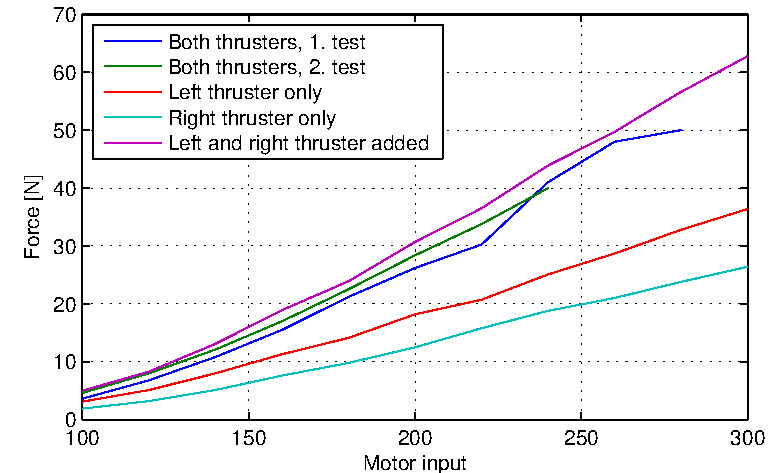
\includegraphics[width=0.6\textwidth]{plot/forwardthrust}
	\caption{Forward motion tests.}
	\label{fig:bollpullforward}
\end{figure}

\begin{figure}[htbp]
	\centering
	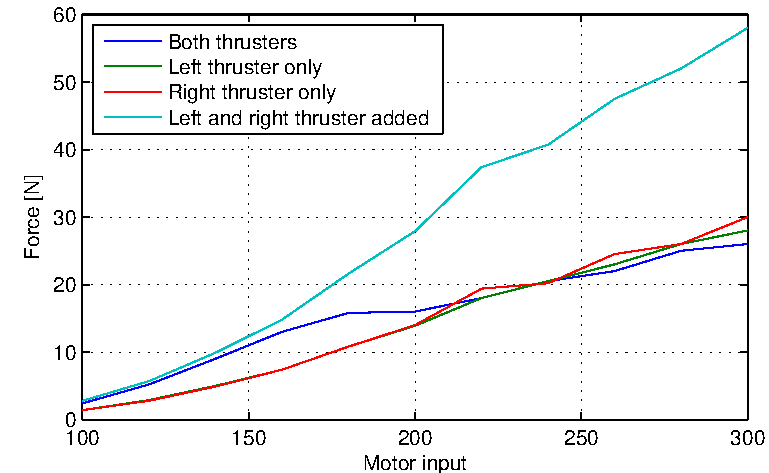
\includegraphics[width=0.6\textwidth]{plot/backthrust}
	\caption{Backward motion tests.}
	\label{fig:bollpullbackward}
\end{figure}

\begin{figure}[htbp]
	\centering
	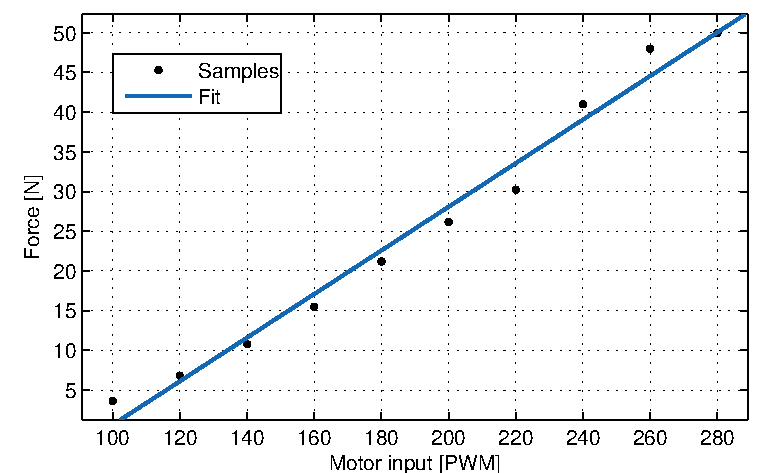
\includegraphics[width=0.6\textwidth]{plot/both_force_1_1order}
	\caption{Forward motion test with 1 order polynomial fitting.}
	\label{fig:1_1order}
\end{figure}

\begin{figure}[htbp]
	\centering
	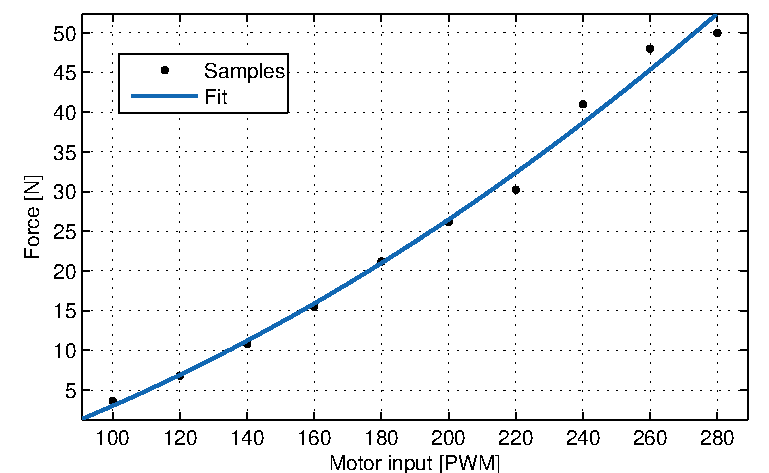
\includegraphics[width=0.6\textwidth]{plot/both_force_1_2order}
	\caption{Forward motion test with 2 order polynomial fitting.}
	\label{fig:1_2order}
\end{figure}

\begin{figure}[htbp]
	\centering
	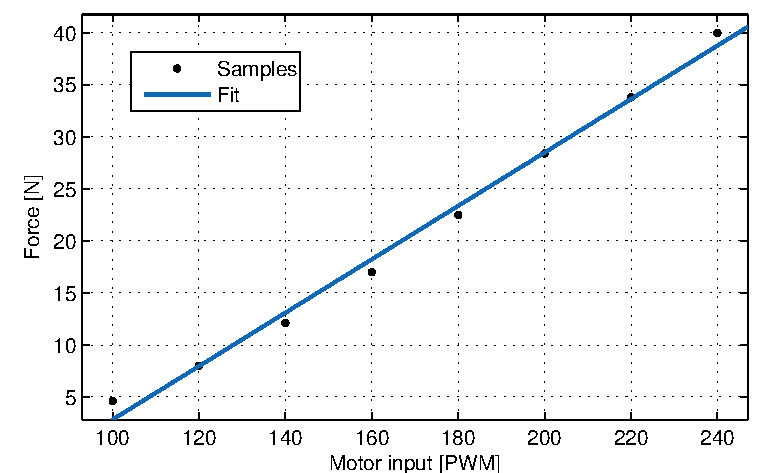
\includegraphics[width=0.6\textwidth]{plot/both_force_2_1order}
	\caption{Forward motion test with 1 order polynomial fitting.}
	\label{fig:2_1order}
\end{figure}

\begin{figure}[htbp]
	\centering
	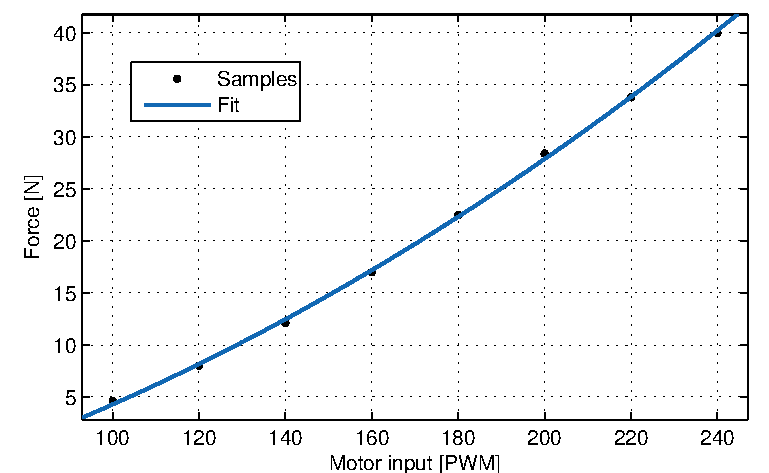
\includegraphics[width=0.6\textwidth]{plot/both_force_2_2order}
	\caption{Forward motion test with 2 order polynomial fitting.}
	\label{fig:2_2order}
\end{figure}

\begin{figure}[htbp]
	\centering
	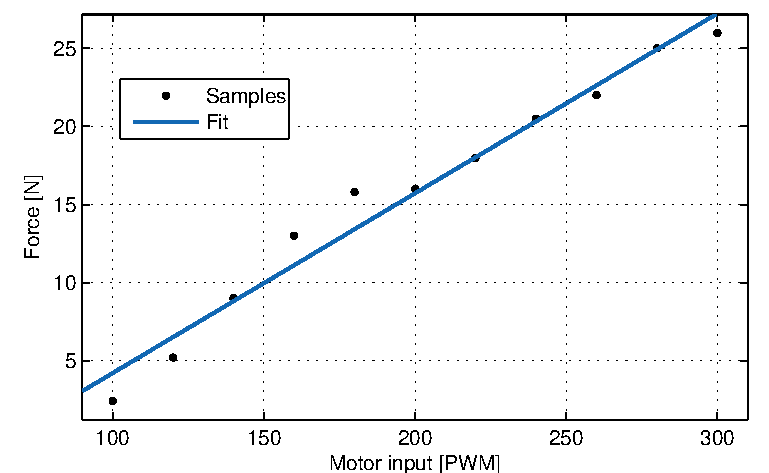
\includegraphics[width=0.6\textwidth]{plot/both_force_3_1order}
	\caption{Backward motion test with 2 order polynomial fitting.}
	\label{fig:3_1order}
\end{figure}

\begin{figure}[htbp]
	\centering
	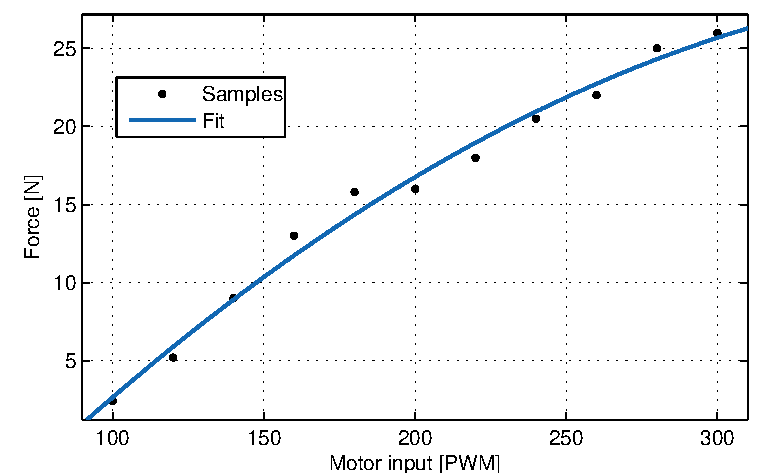
\includegraphics[width=0.6\textwidth]{plot/both_force_3_2order}
	\caption{Backward motion test with 2 order polynomial fitting.}
	\label{fig:3_2order}
\end{figure}

\begin{table}[htbp]
\centering
\begin{tabular}{cccc}
	\toprule
  Test & $R^2$ & RMSE & Function\\
  \midrule
  Both thrusters, forward \ref{fig:1_1order} & 0.9824 & 2.3626 & $f(x)=0.2746\cdot x-26.84$\\
  Both thrusters, forward \ref{fig:1_2order} & 0.9906 & 1.8414 & $f(x)=0.0004976\cdot x^2+0.08552\cdot x-10.52$\\
  Both thrusters, forward \ref{fig:2_1order} & 0.9929 & 1.1513 & $f(x)=0.2567\cdot x-22.83$\\
  Both thrusters, forward \ref{fig:2_2order} & 0.9994 & 0.3638 & $f(x)=0.0005208\cdot x^2+0.07958\cdot x-8.875$\\
  Both thrusters, backward \ref{fig:3_1order} & 0.9729 & 1.345 & $f(x)=0.1152\cdot x-7.318$\\
  Both thrusters, backward \ref{fig:3_1order} & 0.9883 & 0.9383 & $f(x)=-0.0002593\cdot x^2+0.2189\cdot x-16.65$\\
  \bottomrule
\end{tabular}
\caption{Coefficient of determination, Root Mean Square Error and the functions to the fittings.}
\label{tab:fitting}
\end{table}

\section{Discussion and conclusion}
The fitting maps from motor \ac{PWM} input to force output in $N$. When looking at the two first regressions at the forward motion it can be chosen to either use the first order fitting or the second order fitting. The coefficient of determination and the RMSE does not deviate much from the samples in either cases. Thus it is concluded that the first order fitting can be as good as the second order fitting, and the first order is chosen as fitting.

When looking at the regression for the backward motion it can be seen, that the second order fitting estimates the $a$ coefficient of the fitting to be negative. This is due to the backward test. At a \ac{PWM} input above 160 is applied, the vessel starts to ventilate from the propellers. This makes the force, which the vessel's pulls with, be lesser than it actually would if it did not ventilate. Therefore is the first order also seen as the most reliable while going backwards.

\chapter{Verification of attitude with a camera}
\head{This is a description of a technique to verify an attitude
estimator by using a camera. It utilizes the horizon as the reference.}

\section{Purpose}
\section{Method}


While testing it is of importance to make some verifications. When implementing an attitude
estimator for pitch and roll, it is hard to verify that it works as
intended. A simple way to test it is to put the sensor in positions
that can be measured in a static environment, that is by i.e. putting
in on a table on what is to be defined as flat, then angle it
some known degrees and see if the estimator agrees.

Depending on how exotic the estimator is, it might utilise a dynamic
model, in an attempt to improve the accuracy of the estimates. This is
harder to measure in the static lab setup. Another way is to record
the attitude with another setup that is known to work, but that could
not exist, hence the need to implement a new one. Alternatively a
camera can be used, and this is the method to be described in the
following.

One could also use a visual means of determining the heading. The idea
here is to mount a camera on the rigid body object containing the
sensor in the longitudinal direction of the axis of interest. That is
a camera pointing forward for the roll determiniaton or a camera
pointing to one side for the pitch determiniaton. This is intended for
use on ships.

This method relies on a known reference, that is stationary or at least
known at all time. The most ideal scenario is to be in open water
where the horizon is between the sea and the sky. This is guaranteed
to be horizontal, giving us an absolute reference to compare against.

In a non ideal scenario is to e.g. use the harbour quay. This works if
the ship is not moving a lot around relative to the quay, else you
need to know the exact position to the quay to determine the angle the
camera should see as zero. This is also possible but is out of scope
of this description.

\missingfigure{Screenshot of the images generated}

\documentclass[a4paper,11pt,oneside,fleqn]{article}
% Pakker
\usepackage[utf8]{inputenc} % Så må vi bruge æ, ø og å
%\usepackage(ansinew){inputenc}
%\usepackage(danish){babel} % Dansk opsætning
\usepackage[T1]{fontenc} % Hjælper med orddeling ved æ, ø og å. Sætter fontene til at være ps-fonte i stedet for bmp.
\usepackage[english,final]{varioref} % Vi kan anvende \vref
\usepackage{array,booktabs} % Til gode tabeller
\usepackage[printonlyused,withpage]{acronym} % Smart akronymhåndtering
\usepackage{minitoc} % Vi kan lave del inholdsfortegnelser forhåbentlig
\usepackage{graphicx} % We can now use \includegraphics and stuff
\usepackage[svgnames]{xcolor} % Colored stuff i.e. \colorbox
\usepackage{pdfpages} % Inkludere en pdf side som en side  
\usepackage{amsmath,amsfonts,amssymb} % God matematik
\usepackage{wasysym}% smileys
\usepackage{textcomp} % More text stuff, such as numero
\usepackage{mathtools} % We can now use \xRightarrow{hello world}
\usepackage{booktabs} % Rulers for tables
\usepackage[thinspace,amssymb]{SIunits} % Using macros for typesetting SI units
\usepackage{natbib} % Use proper citation
\usepackage{tocbibind} % Includes toc and bib in toc
\usepackage{listingsutf8} % Code listings
\usepackage{tabularx,booktabs} % Tables with fixed width
\usepackage{todonotes} % Todonotes
\usepackage{tcolorbox} % Colored boxes!
\lstset{extendedchars=\true, inputencoding=utf8/latin1} % This and listingsutf8 makes us able to use utf8 and latin1 as inputfiles
\lstset{language=matlab,frame=single,basicstyle=\footnotesize\ttfamily}
\usepackage[pdftex]{hyperref} % Hyperlinks
\hypersetup{backref,
bookmarks=true,
bookmarksnumbered=true,
colorlinks=true,
linkcolor=Navy,
citecolor=Green} % Setting some fancy colors
\DeclareUnicodeCharacter{00A0}{~} % Fix odd OSX/textwrangler no break space charater
\newcommand{\head}[1]{\vspace{3mm}{\noindent \hspace{-0.5em} \fcolorbox{gray}{GhostWhite}{\parbox[c]{\textwidth}{\slshape{#1}}}\vspace{2mm}}} % Header

\let\oldhat\hat
\renewcommand{\vec}[1]{\boldsymbol{#1}}
\renewcommand{\hat}[1]{\oldhat{\mathbf{#1}}}

\newcommand{\MATLAB}{M{\footnotesize ATLAB}}

\begin{document}
% Frontpage
\author{Nick Østergaard}
\title{Users Manual\\
	for\\
\emph{ASV Formation Control for Surveying Purposes}}
\date{\today}
\maketitle
\thispagestyle{empty}
\begin{center}
	\includegraphics[width=13cm]{fig/aauship}
\end{center}
\vfill
\begin{center}
	
\includegraphics[width=5cm]{fig/AAU_LOGO_CMYK_UK}\\
	Department of Electronic Systems
\end{center}
\clearpage

% Abstract
\begin{abstract}\addcontentsline{toc}{section}{Abstract}

This report documents the design and implementation of optimal control
of a helicopter test setup controlling the travel and elevation with
and without feedback using a linear quadratic controller.

The helicopter model has 3 degrees of freedom, controlled by two
horizontal propellers to adjust pitch and elevation, nonzero pitch
makes it travel.

The implementation is done in \MATLAB\ and with QuaRC from Quanser
integrated with Simulink and MathWorks' Real-Time Workshop. The code
and simulink models are also presented in the appendix.
	
\end{abstract}


% Table of contents
\tableofcontents
%\listoftables
%\listoffigures
\newpage

% Inclusion of body text here
\chapter{Introduction}
\head{In this chapter is the motivation for the project stated and the previous work within the subject will be summed up.}

\section{Motivation and the AAUSHIP Project}
The Port of Aalborg would like Aalborg University to help them to expand their options of improving the conditions of the Limfjord. One of their tasks is to map the seabed of the Limfjord to get bathymetry data. This will help them guide larger cargo ships to port while using the autonomous ships as guidance.

Another aspect from The Port of Aalborg is a task to escort larger ships with cargo into The Port of Aalborg. This is done by a pilot whom needs to sail out to incoming larger cargo ships and escort them safely into port. The pilot does this in a pilot boat which is controlled manually by the pilot. The Port of Aalborg would like this process to become autonomous such that an autonomous boat can sail to the cargo ship and to some extend take over the control and guide the cargo ship into port. The system to do this implies that The Port of Aalborg needs an autonomous ship which can perform this task.

The mapping itself can be done by one ship or by more. For the moment one of the ships from The Port of Aalborg, which is manned, and covers the mapping of the closer part of the Limfjord ($\approx$ 65 km). This is only done every third year, but mapping around Hals Barre (a sandbar \todo{slet efterfølgende kommentar igen engang}and not a beach bar) at the end of the Limfjord is a more critical place and is mapped every third month.

If The Port of Aalborg had an autonomous ship fleet at their disposal, which could sail out and do the mapping autonomously, they would get updated bathymetry maps with a higher update frequency than they have currently \citep{portofaalborg}. This will result in a digitalizing of the seabed, a digital map, which has different implementation options by The Port of Aalborg.

This thesis will utilise formation control and extensions to manoeuvre agents through a specified area for surveying purposes. The aspect of formation control is chosen due to the rather large areas that The Port of Aalborg needs so cover. When applying formation control it is assumed to be faster to cover a larger area than if one single boat needed to scan the area. The formation that are to be chosen depends on the specific area of interest, which could e.g. be inside the harbour or around the pillars of the bridge. Chapter~\vref{ch:formcontrol} will introduce what kind and scopes of formation control that exists today. These theories makes the basis for the formation control within the scope of this project.

As a future scope this can be used when making a model of the seabed of how this will get sanded. This model can tell The Port of Aalborg when to go clean the seabed. The AAUSHIP project can be used to verify this model, such that The Port of Aalborg do not have to go out with equipment to solve the sanding without the need of it.

\section{The Mission}
\label{sc:mission}
Within the scope of this project the robots will be unmanned ships,
\ac{ASV}. The ship's main purpose will be to map the seabed by using
sonars to obtain bathymetry data. When one ship need to do this alone, and due to the range of
the sonar, the time spend could be improved by using multiple ships. The sonar scanning would
be done as seen on figure~\vref{fig:concept-art}.

\begin{figure}[htbp]
	\centering
	\subfloat[One ship\label{fig:concept-art1}]{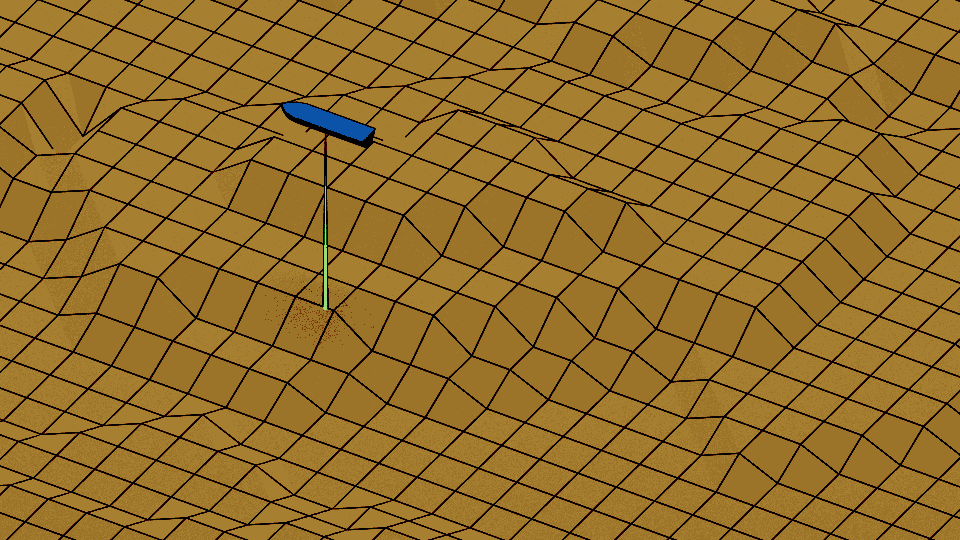
\includegraphics[width=0.48\textwidth]{fig/conseptart-single}}
	\ % One forced space to seperate figures
	\subfloat[Thee ships\label{fig:concept-art3}]{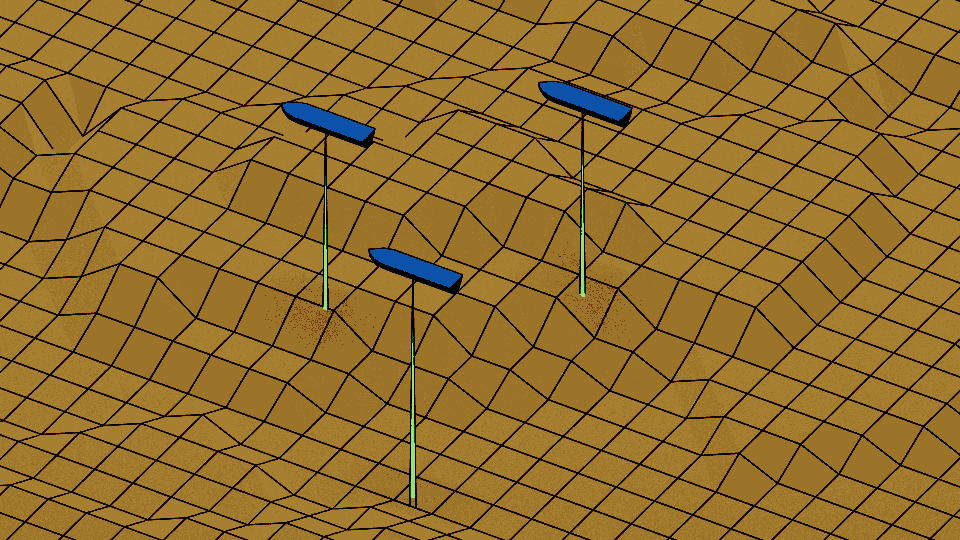
\includegraphics[width=0.48\textwidth]{fig/conseptart-formation}}
	\caption{Comparison of two ways to cover an area with a lawn mower
	pattern.}
	\label{fig:concept-art}
\end{figure}

When only one ship (figure~\vref{fig:concept-art1}) need to map a complete seabed this process could
take up much time dependent on the area that need to be covered. The
time spend could be improved to make this mapping more efficient. One
way of optimizing the time used is to add more ships (figure~\vref{fig:concept-art3}) to help map the
seabed. To make the process of this as optimal as possible it could be
of benefit to implement formation control in the specific assignment.

I cooperation with the port of Aalborg, a use case is presented, where we can perform tests of the platform, and use those to compare the performance of our system to their system.
\begin{figure}[htbp]
	\centering
	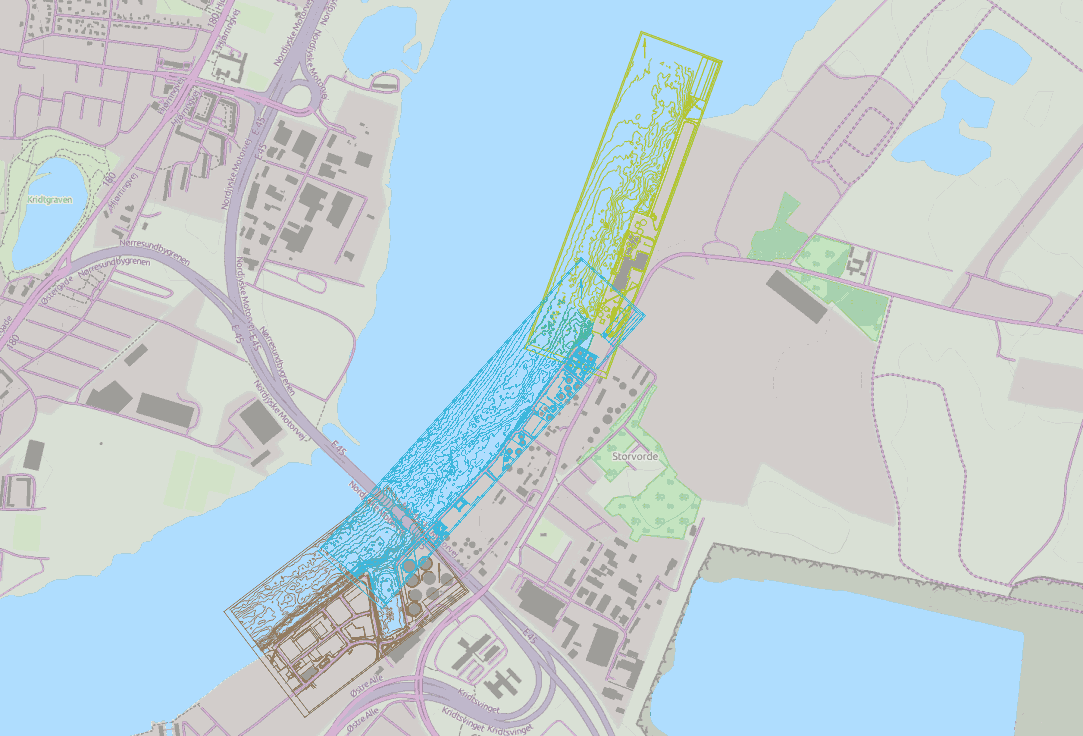
\includegraphics[width=\textwidth]{fig/use-case-data}
	\caption{Area of the harbour at Aalborg Portland provided as sample
	data from Aalborg Havn. Background map data CC BY-SA OpenStreetMap.}
	\label{fig:diffforms}
\end{figure}

When performing this kind of surveying with multiple ships, it is important to take note of the kind of sensor it uses and the coverage that it provides. Initially the port of Aalborg used single beam echo sounders, but have in recent years turned over to multibeam sonars for their survey boat, which has improved their resolution and time for a survey. But they still wishes to improve the survey update rate, by e.g. using fairly low cost autonomous ships to get better indication of the seabed to identify if an expensive thorough survey is needed. An image of the survey vessel they use now used can be seen on figure \ref{fig:alba}. As it can be seen, this survey vessel is relatively large, being over 20 metres long. To comparison is the AAUSHIP only 1.1 metres long. For surveying in smaller areas, like inside the harbour area, Aalborg Havn uses a smaller scale vessel which is 12 metres long. This vessel is only used at the smaller areas thus not the one being used out in the Limfjord close to Aalborg.
\begin{figure}
	\centering
	\includesvg{alba}
	\caption{The survey vessel used by Aalborg Havn named Alba.}
	\label{fig:alba}
\end{figure}



%This could be done in several ways, but is mostly thought of in a
%rigid formation, such that the formation maps the same area of the
%seabed the whole time. The idea can be seen on
%figure~\vref{fig:concept-art}.

\section{Objective}

\head{This section describes what can be done for humanity by the use of
automation in the realm of Aalborg.}

A use case that is a basis of this project is a service that surveying
companies offer, which is to survey and map the seabed of waterways and
lakes. Currently they do this very manually my sailing with a boat in
the lake after a \ac{GNSS} in the boat. In waterways as small rivers
and the like in Denmark they do it by a smaller boat or raft, where
they are using a prism system and a stick to take point measurements
of the river.

These tasks could be automated and probably improve surveying time by
using an autonomous system that can cover this. Here focus is on
trying to design such a system with small ships sailing in formation
to scan a predefined area.

This will then lead to defining the needed capabilities for
the formation control.

\todo{See 3.3.2 in \citep{thorvaldsen} for some nice definitions.}

\chapter{General formation control}
\head{This section will give a short introduction to formation control in general, by discussing existing formation control paradigms and relating them to the motivation of the AAUSHIP as a survey platform consept.}

%\head{Formation control in general is concerned with simultaneous control of dynamic systems. These systems is often referred to as agents where the objective of these is to maintain a static reference to a specified object. This object could be another agent witch then would be referred to as the leader. The other agents objective will then be to stay in the relative position to the leader within a static formation.}

The theory of formation control in general is widely applied. It is usually applied in assignments regarding control of robots which needs to be placed relative to each other. Depending on the given task of the robots, and which type of robots are in focus, the formation can be utilized in different ways \cite{muv-survey1}.

The robots can also be of various types: Driving vehicles, helicopters, aeroplanes, ships etc. which can be both manned and unmanned. The tasks that these robots needs to fulfill can vary greatly. Robots in groups in general have many purposes such as vacuum cleaning robots, who needs to clean a rather large area or flying swarm robots like quadcoptors who can make different kinds of assignments. When quadcoptors work as a combined group they could lift a certain amount of payload to achieve their goal as a group, or they could work individually in a network to do several smaller tasks. An example of how quadcoptors are working together can be examined at \citep{ethswarm}.

All the robots in the terminology of \cite{muv-survey} are called \textit{agents}. These agents move either individually or in formation. This formation can be rigid or be flexible. If the agents move in rigid formation they will keep their relative positions to each other and must not diverge from the formation. The formation could also be flexible which sometimes is preferable. If the distances between three agents on line are large, and an obstacle needs to be avoided, only one of the agents needs to move from this obstacle if the formation is flexible. This can be seen on figure~\vref{fig:form_avoid_right}.
\begin{figure}[htbp]
	\centering
	\includesvg[width=0.5\textwidth]{form_avoid_right}
	\caption{A flexible formation where the right agent avoids an obstacle.}
	\label{fig:form_avoid_right}
\end{figure}

\section{State of the art}
When looking into formation control many different types of control can be taken into control. The main types of formation control are separated into six different types, separated by \cite{muv-survey}, all under the main topic \textit{multiple vehicles coordination strategies}. The overview for this can be found in the survey paper \cite{muv-survey} who explains the six main types and a few alternations of these.

The theoretical views on control of \ac{MUV}'s behaviour are by \cite{muv-survey} divided into two classes; centralized and decentralized systems. If the system is centralized this means that all control of the formation is done on one agent, and the others receive information from the core agent. This form of system has the advantage that the core agent can optimize vehicle coordination, accommodate individual agent faults and monitor the accomplishment of the mission. The main disadvantage of this system is that if a fault should occur in the core agent this will affect and facilitate a failure of the whole system.

The opposite way of controlling the system would be in a decentralized way. This way of controlling the formation is inspired by the aggregation of birds and fish. This makes each agent able to communicate and share information in between. This means that each agent is given its own part of the complete objective and thus can only complete a part of it, like moving around an object to get to end point of a trajectory. The advantage is that faults in a single agent can be overlooked, thus more robust to faults, but can result in a less efficient objective outcome. A decentralized system may be more appropriate to scale up such that more agents can be included and the computational load can, in difference from the centralized system, be split up onto more agents.

The different types of coordination and control algorithms within centralized and decentralized systems include: \textit{behavioural-based}, \textit{virtual structure}, \textit{leader-follower}, \textit{graph-based} and \textit{potential field approaches}. Within these structures are the terms \textit{cooperation control} and \textit{formation control} used. Cooperative control focuses on the global task that the group of agents needs to fulfil, and the formation control is the actions performed by each agent which is shared with the other agents in the group. 
\begin{description}[style=nextline]
	\item [Virtual structure]
	In a virtual structure is the entire formation treated as a single entity. The behaviour coordination for a group of agents in a virtual structure is uncomplicated compared to the coordination of many agents, due to the making of one structure e.g. based on fixed distances between the agents. The disadvantage falls on the centralization due to the structure treated as a single entity. If a failure in this structure happen results in a failure in the entire structure.
	\item [Behaviour Based Methods]
	The behavioural based model employs several behaviours for each of the agents and the final control used to control the formation is derived from a weighting of the relative importance of each of the behaviours. This could for instance be navigational behaviours to enable a navigation to be the main goal while avoiding hazards and stay in formation. So if one agent needs to avoid a collision with an obstacle the rest of the group should not take this into account. Only that single ship needs to leave the formation and get back into formation again.
	\item [Leader-Follower Approaches]
	Applying leader-follower methods designates one agent as being the leader and the rest of the agents as followers. The following agents need to position themselves relative to the leader and maintain a desired relative position to the leader. This makes the simplicity to this method, but there is no feedback from the followers to the leader and thus makes that a disadvantage. Separation-separation and separation-bearing are two popular leader-follower formation controls, where the followers stay at specified separation and bearing from their designated leader. Within this method it is possible to split the group up into several smaller groups with their individual designated leader.
	\item [Potential Field Approach]
	Potential field approaches assigns potentials to agents to make a weighting between them. This weighting could for instance determine the relative distances between the agents. This is usually used when following a virtual leader, such that this process is only made relative to the agents within the structure. This method can make ensure a collision free formation when every agent has been assigned their potential weighting respectively. In this method obstacles can be included and have assigned potentials as well. This will become an avoidance radius from the specific object.
	\item [Graph Theory Approaches]
	When applying the graph theory method one assign every agent as a node and assign connections between the nodes. In graph theory this is denoted vertices and edges. The study with graph theory is mainly concentrated of the formation itself and related to changes within the structure. This can be related to the structure within a tree-structure which is used when assigning the formations in graph theory manor. This can be applied as communication analysis for the agents and consensus analysis can be of benefit. The edges between the nodes symbolizes the possible connections thus communication between them. The nodes that are connected are denoted as neighbours and are capable of communicating.
\end{description}

\subsection{Approaches on formation control}
When performing this kind of surveying with multiple ships, it is important to take note of the kind of sensor it uses and the coverage that it provides. Initially the port of Aalborg used single beam echo sounders, but have in recent years turned over to multibeam sonars for their survey boat, which has improved their resolution and time for a survey. But they still wishes to improve the update rate, by i.e. using fairly low cost autonomous ships.

\missingfigure{Picture of the port of Aalborg's survey boat.}

This does not have any relevant impact of how the mappings of the seabed would be due to the subsequent processing of the collected data from the maps.

Different formations of ships can be seen on figure~\vref{fig:diffforms}.
\begin{figure}[htbp]
	\centering
	\includesvg[width=0.5\textwidth]{diffforms}
	\caption{Different formations which the \ac{ASV}s can make.}
	\label{fig:diffforms}
\end{figure}

The formation of the ships may not need to be strictly rigid. Situations could appear where it would be of benefit to change the ship's formation. If the formation need to avoid an obstacle and one or more ships needs to go faster or slower, which leads to a change in the formation, it might be of benefit to regroup the formation which is faster to reach. An example can be seen on figure~\vref{fig:avoid}.

\begin{figure}[htbp]
	\centering
	\includesvg[width=0.5\textwidth]{form_avoid}
	\caption{A formation needs to go around an obstacle where the inner most ship chooses the shortest path and the formation regroups.}
	\label{fig:avoid}
\end{figure}

When doing the formation control it is important to figure out what one
want to achieve, and depending on the strategy and the formation type
some things are to be considered as requirements regarding how the
formation should work. In this discussion lawnmower patterns are considered. In this work thee ships are considered for simplicity, but it should be extensible to n-number of ships. The lawnmower patterns will suit well for the mapping of a seabed where one or more ships are to sail from shore to shore in a fjord.

\subsubsection{Initialisation}
When looking at the specific task several things needs to be taken into account. When starting the mission, the ships may start at positions that is not in the desired formation. It might be of importance that the ships are in
formation when they start tracking the desired track. Therefore some
attention must be given on how to make the ships initialize this
formation. This is referred to as the group coordination task. An approach is to make the ships sail individually to the
starting positions with a speed that makes them hit their respectively starting points at
the same time. If one reaches its start point much earlier
than the other it must stop, which is not wanted because it then can
drift out of position again. This basically means that there exists an initialization
phase and a tracking phase. The start heading should of
course align with the path at the start point such that the path following can begin with zero error. The ships could also target their group formation before starting at time zero at the path. This will eventually make the initialization take longer time but ensure that the ships have made the group coordination task and are ready to start at the path.

Another issue to be considered is to ensure that no ship at
any point in time reaches a minimum speed that is necessary for the
ship to not drift out of formation. This could be a problem in corners
of the formation if a stiff construction, where the inner most ship
has to move slower, to accommodate the shorter distance on an inner
circle arc.

Faults like blackout on a ship could also be considered in the control
design. I.e. what happens with the formation when one ship faults in a
blackout. Should the rest of the formation stop, should the formation
still follow this drifting ship or should the mission simply terminate
when it is discovered that a ship has blackout. This is under the assumption that the formation is decentralized and every ship has its own control and is not controlled from a mother ship.

In the initialization phase it is also relevant to consider how the
ships should avoid each other if they are on the wrong side of each
other. If it is of benefit that a specific ship is at the most inner route, and is located at an outer position before the group coordination, this ship needs to cross the formation to get to the desired starting position. This initialization needs to be adjusted in the initialization phase to ensure that no ships collide.

\begin{figure}[htbp]
	\centering
	\includesvg[width=0.4\textwidth]{cornoring}
	\caption{Two ships initializing and following the path offset
		equally on each side, ships are constrained to sailing parallel
		and heading the same as path when projected onto the path. Blue
	dot is start of path. Fully drawn splines is initializing phase.}
	\label{fig:cornoring}
\end{figure}

On figure~\vref{fig:cornoring} is a simple path following performed
with two ships in a stiff formation with an equal distance from the
path. It illustrates four steps. In step \#0 the ships initializes a
random position near the start of the path being the group coordination task. At \#1 it is tracking the
path in formation, whilst still in formation. This is referred to as a formation coordination task. At \#2, the green
(right) ship is in a tight inner curve where it is important to
consider design of the path such that the capabilities of the ship is not
exceeded to stay in formation. At \#3 it is back to straight line path
following in formation. \citep{thorvaldsen}.

\begin{figure}[htbp]
	\centering
	\includesvg[width=0.6\textwidth]{form_rigid_90}
	\caption{Three ships in formation needs to make a 90\textdegree turn and stays in their relative positions and keeps the rigid formation.}
	\label{fig:form_rigid_90}
\end{figure}

When the ships needs to make a turn about something they can do it in many ways. On figure~\vref{fig:form_rigid_90} the ships keep their formation whilst turning about the object. When they reach the other side and have finished their turn, the ships have kept formation but the outer most ship has now become the inner most ship. The reason to turn like this could be that the inner most ship, the yellow ship, cannot turn as sharp as demanded to stay the inner most ship. Therefore, instead of turning the formation, they stay geometrically rigid.

\begin{figure}[htbp]
	\centering
	\includesvg[width=0.6\textwidth]{form_change_90}
	\caption{Three ships in formation needs to make a 90\textdegree turn and changes their relative positions.}
	\label{fig:form_change_90}
\end{figure}

As seen on figure~\vref{fig:form_rigid_90} the ships could have benefit of turning like this. This way of turning could cause trouble in the top of the turn, where the ships eventually will collide due to errors and the relative close distance to each other. This way could be altered a little such that the ships will turn like on figure~\vref{fig:form_change_90}. There the ships adjust their position and velocities to ensure that they will not collide, but they will therefore leave their formation shortly to return back into position again.

\subsubsection{Degree of Actuation}
The degree of actuation is a matter that sets some limitations on how
the path following can be made, and thus the methods available to
control the ships.

AAUSHIP is a ship, which means that is is not fully actuated in the
whole 3D space, but this is not needed since it is moving on a
surface. To be fully actuated it must be able to have controls for
surge, sway and yaw.

There are different ways of controlling, and a few could be:
\begin{description}[style=nextline]
	\item [Three or more controls]
	When having three or more control parameters it is said that the vessel is fully actuated. This way of controlling is usually used in low-speed manoeuvring and stationkeeping mostly by offshore \ac{DP} vessels.
	\item [Two controls and Trajectory-Tracking control]
	Trajectory-Tracking is done in a three \ac{DOF} system, $e(t)\in\mathds{R}^2\text{X}S$. It is done with two control inputs, $u(t)\in\mathds{R}^2$. This means that the control problem is underactuated which cannot be solved by linear control theory. A vessel under these terms is able to manoeuvre along a path with constant sideslip angle using only surge and yaw. This is the classic approach for path following.
	\item [Two controls and Weather-Optimal heading]
	When taking the weather conditions, and in general the environmental disturbances, into account, it is done as a mean of all the disturbances. This is used to stabilize the vessel regarding the position. It is done by making the heading depend of the change in the mean of the environmental disturbances.
	\item [Two controls and Path-Following control]
	The standard way by having two controls, being surge and yaw, and achieving path-following, is to define a 2-D workspace. This workspace is placed along the trajectory with along-track and cross-track vectors that are to represent the error to minimize. This is usually done by applying the \ac{LOS} path following controller that makes use of surge and yaw to accomplish the path following. This implies that a six \ac{DOF} system model needs to be internally stable such that only the two control inputs are used.
	\item [One control]
	This is only done with systems with three \ac{DOF} and is normally only used to stationkeeping.
\end{description}
\citep{fossen}

\subsection{Delimitations}
Within the scope of the AAUSHIP project will the focus be to apply and extend a leader-follower approach at the ships. This will include several tasks. The two main tasks will be to make a group coordination task and a formation coordination task. The group coordination task will be, as described earlier, an objective to get the ships into the desired formation before or exactly at the starting point of the path following. The formation coordination task will be to make a leader, virtual or not, follow a predetermined path set by waypoints. The path should be generated from waypoints placed on a map due to that the ship needs to travel over larger distances. This will make a waypoint based follower where the path will be generated between the placed waypoints.

The placement of the waypoints will be placed such that the ships need to surge along a lawnmower pattern, where the turns have a lower requirement of turn radius dependent on the surge velocity of the most inner ship. This is due to the drift if the inner ship looses too much velocity.

When applying the leader-follower approach it needs to be determined how the formation precisely should be set up. In this project is only one leader considered at a time. The rest of the ships will act as followers to the leader. The idea can be seen on figure~\vref{fig:l_f} where only one leader is represented with a single or more followers.
\begin{figure}[htbp]
	\centering
	\includesvg[width=0.6\textwidth]{lead_follow}
	\caption{A leader is always assigned and potential followers are following.}
	\label{fig:l_f}
\end{figure}
When the followers are in formation with the leader is only the leader who is following a specified trajectory. The other ships, the followers, only keeps their position relative to the leader. This makes the predetermined formation moving along the path relative to how the leader is following the path. The leader is autonomous as well as the followers, but the path following is only done at the leader and the followers maintains their relative positions to the leader.

If the leader diverges from the path, drifting to the left, this will result in the whole formation drifting to the left. This problem can be dealt with in different ways, e.g. the control could react fast enough to make the formation get back on track within a specified time, or some fault tolerance could be done from the whole system. If the leader diverges from the path it could make the formation stay at their respective headings within a time slot before actuating towards the leader.

The formation needs to take into account if it is of benefit to change leader. If some kind of obstacle makes the formation turn about it, it might come to benefit to change the leader which needs to be done on the fly. This entails a change in the group coordination and the ships needs to set their relative position and heading from another ship.

The configuration of the formation will be set up, as a start, with one leader and a single follower. The follower will be offset from the leader with a distance of five metres. This can be seen on figure~\vref{fig:l_f1}.
\begin{figure}[htbp]
	\centering
	\includesvg[width=0.4\textwidth]{lead_follow1}
	\caption{The leader with a follower offset by 5 metres radius.}
	\label{fig:l_f1}
\end{figure}
This will be a rigid formation that the ships needs to keep at all times. The change of leader will eventually be taken into account when the ships needs to turn. If the formation needs to turn clockwise about it might be of benefit to change the leader. 

The location to test and implementation the AAUSHIPs will be in the Limfjord. The optimum will be to make the formation go across the Limfjord and back in lawnmower pattern and make measurements of the seabed. Due to the location where it is presumed to have enough space, the formation is not of bigger importance to the mapping. The only important thing to include regarding the formation is that the ships needs to be able to turn around without loosing so much velocity such that they start drifting and offset the formation.

\section{Notation}
For convince this section defines notation that is used throughout
this manuscript.

\subsection{Reference Frames}
When working with dynamical systems that move in space, such as the
ship, it is convenient to work with different frames of reference, and
this means that a proper notation has to be used. 

\citep{fossen}

\begin{table}[htbp]
	\centering
	\begin{tabular}{llccc}
		\toprule
		    & & Forces and & Liner and          & Positions and  \\
		DOF & & moments    & angular velocities & Euler angles   \\ 
		\midrule
		1 & motion in the $x$ direction (surge)       & $X$ & $u$ & $x$ \\
		2 & motion in the $y$ direction (surge)       & $Y$ & $v$ & $y$ \\
		3 & motion in the $z$ direction (surge)       & $Z$ & $w$ & $z$ \\
		4 & rotation about the $x$ axis (roll, heel)  & $K$ & $p$ & $\phi$ \\
		5 & rotation about the $y$ axis (pitch, trim) & $M$ & $q$ & $\theta$ \\
		6 & rotation about the $z$ axis (yaw)         & $N$ & $r$ & $\psi$ \\
		\bottomrule
	\end{tabular}
	\caption{\cite{sname1950} notion for marine vessels, from
	\citep[table~2.1]{fossen}}
	\label{tab:sname}
\end{table}


\section{Preliminaries}
As a means to present the methodology used in this it is important
to use a terminology that is easy to understand and not conflicts too
much with the reaferences. There fore this sections will describe some
of those.

Firstly for formation control there is two main tasks that is in a
basic formation control setup, and as describen in \citep{thorvaldsen}
he uses two terms to describe the overall task \textit{Formation
Control Problem} as the  \textit{Group Coordination Task} which is the
task where it to make the group form the initial formation, and then
the \textit{Formation Mission Task} which is the task of moving the
formation on the desired path. \todo{Ligende illustration som fig 3.1
	fra \citep{thorvaldsen} her.}


\section{Parts list}
See table~\vref{tab:parts}.
\begin{table}[htbp]
	\centering
	\begin{tabularx}{\textwidth}{ll}
	\toprule
	\# &  Model \\
	\midrule
	2 & Graupner InIine 750 \\
	2 & Electronic Speed Controller \\
	2 & Propellers \\
	2 & Prop Shaft \\
	2 & Motor to prop shaft couplings 5mm\\
	6 & LiPo 3600 mAh 4S1P batteries \\
	1 & Intelligent Charge Port (ICP) \\
	1 & Raspberry Pi or similar \\
	1 & 4-split USB hub\\
	1 & Echosounder \\
	\bottomrule
	\end{tabularx}
	\caption{Mechanical parts for an AAUSHIP}
    \label{tab:parts}
\end{table}


\section{Power System}

The power source in AAUSHIP is chosen to be LiPo batteries, which is
a type of battery chemistry where the operator take great care in not damaging
the batteries. If care is not taken they might catch on fire, which
cannot easily be extinguished. This can of course be dangerous.

\subsection{Power Harness}
The power system on the ship consists of some somewhat convoluted
wiring harnessed loosely in the hull structures. An single line
diagram is therefor provided to give an overview of the system.

\begin{figure}[htbp]
	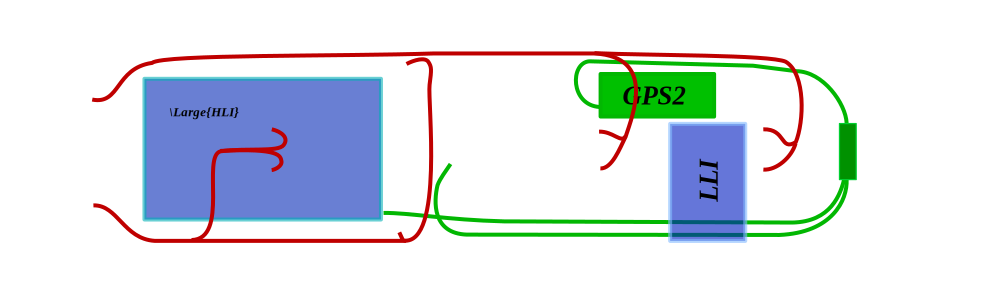
\includegraphics[width=\textwidth]{fig/harness}
\end{figure}

\subsection{LiPo Basics}
The LiPo battery packs each consists of four cells in series, which in
the LiPo battery world is called ``4S1P''. One parallel is what you get
when you only have a series connection.

Since each cell is normally not charged individually but across the
output terminals of the battery, every pack with more than one series
cell is equipped with a so called balance port. This is basically a
smaller multiple pin connector that has a connection to each cell,
such that is is possible for a ``balancer'' to discharge cells that is
unbalanced. An unbalanced cell is basically just a cell that does not
have the same voltage as the others.

This balancer is usually run whilst one is charging the main
connections. The purpose is to eliminate the difference that is
inherent in each cell not being exactly the same, such that one cell
does not get overcharged, when charging them in series.

\subsection{LiPo Battery Safety}
\begin{tcolorbox}[colback=yellow!75!,colframe=red]
It is strongly advised not to mess with the LiPo batteries before you
have read and understand how to handle them. A good resource for
learning some basics and safety about LiPo batteries are
\citep{tjintech:lipo-basics} and \citep{tjintech:lipo-safety}.
\end{tcolorbox}
 

\appendix
\chapter{Acronyms}
\label{ch:acronyms}
\begin{acronym}[TDMA]
%\begin{acronym}[HBCI]
	\acro{AAU}{Aalborg University}
  \acro{ASV}{Autonomous Surface Vessel}
	\acro{ADC}{Analog to Digital Converter}
  \acro{AHRS}{Attitude and Heading Reference System}
  \acro{BODY}{The body frame}
  \acro{CFD}{Computational Fluid Dynamics}
  \acro{DOF}{Degrees-Of-Freedom}
  \acro{DP}{Dynamic Positioning}
  \acro{ECEF}{Earth-Centered Earth-Fixed} 
  \acro{ECI}{Earth-Centered Inertial}
  \acro{EKF}{Extended Kalman Filter}
  \acro{FRF}{Formation Reference Frame}
  \acro{FRP}{Formation Reference Point}
	\acro{GNC}{Guidance, Navigation and Control}
  \acro{GNSS}{Global Navigation Satellite System}
  \acro{GPS}{Global Positioning System}
  \acro{GRS}{Ground Segment}
  \acro{HLI}{High Level Interface}
  \acro{IMU}{Inertial Measurement Unit}
	\acro{IP}{Internet Protocol}
	\acro{IPv4}{Internet Protocol version 4}
	\acro{IPv6}{Internet Protocol version 6}
  \acro{KF}{Kalman Filter}
  \acro{LKF}{Linear Kalman Filter}
  \acro{LOS}{Line-Of-Sight}
  \acro{LLI}{Low Level Interface}
	\acro{LSB}{Least Significant Bit}
  \acro{LTI}{Linear Time Invariant}
  \acro{MARG}{Magnetic, Angular Rate, and Gravity}
  \acro{MMSE}{Minimum Mean Square Error}
  \acro{MUV}{Multiple Unmanned Vehicle}
  \acro{MPC}{Model Predictive Control}
  \acro{NED}{North-East-Down}
  \acro{OSM}{OpenStreetMap}
  \acro{PWM}{Pulse Width Modulation}
  \acro{ROS}{Robot Operating System}
  \acro{RTK}{Real Time Kinematic}
  \acro{SOG}{Speed Over Ground}
  \acro{SSS}{Single Screw Ship}
  \acro{SSM}{State Space Model}
  \acro{TSS}{Twin Screw Ship}
  \acro{UGAS}{Uniformly Globally Asymptotically Stable}
  \acro{UGES}{Uniformly Globally Exponentially Stable}
  \acro{UGS}{Uniformly Globally Stable}
  \acro{UKF}{Unscented Kalman Filter}
  \acro{WGS84}{World Geodetic System 1984}
\end{acronym}



% Bibliography
\bibliographystyle{apalike}
\bibliography{bib}\label{sec:bibliography}

\end{document}

\chapter{Battery Monitor for AAUSHIP}
\label{ch:bm}

\head{This appendix is a minor chapter describing a hardware
	component, the battery monitor, for AAUSHIP which was also devised
	under the project period. This is not directly a goal according to
	the project thesis, hence this is included in the appendix for
	referencing.}

Since the AAUSHIP is equipped with multiple LiPo cells, it is of high concern to have a means of checking the state of these battery cells.
Therefore a battery monitor have been created, that can be hooked onto the
\ac{LLI} via the I$^2$C bus. This will enable the \ac{HLI} to report
the voltages on the cells. This was implemented with \ac{ROS} by
utilizing the graphical interface for \ac{ROS} called rqt. In this Qt
based environment it is possible to make plugins as easy as it is to
create \ac{ROS} nodes. A screenshot of the plugin in action is seen
on figure~\vref{fig:bm-rqt}.

The battery monitor is made of two \ac{ADC} chips, both being the MCP3428,
each with four channels and 16-bit resolution. But not all this
resolution is of real use as such, because it is implemented with a
resistor voltage divider from each cell in series, which basically
means that only the top end of the value range is used. 

It is designed to measure maximum 4.2 V per cell to the minimum
allowed voltage of about 3.6 V per cell. It can of course measure
smaller values but the critical value is around 3.6 V. The four cells are connected in series, each with a resistor divider with
reference to the negative lead. The division ratio is determined by
the maximum voltage present at the cells (which is in series with the
lower ones), such that the cell voltages are at the two volt that
each \ac{ADC} can handle. This gives the following ratios for the
cells:
\begin{align}
	\#1 = 0.12, \quad \#2 = 0.16, \quad \#3 = 0.24, \quad \#4 = 0.48
\end{align}

This means that the voltage on high cell \ac{ADC} is ranging from
about 1.728 V to 2.0 V. In turn meaning that the reading will only use
the top 15 \% of the capabilities of the \ac{ADC}. This results in a
range for the high side \ac{ADC} of about 288 when using the exact
numbers, which equates to about 8 mV per \ac{LSB}. The lower ranges
are more accurate.

High resistance dividers is used since these are always connected to
the battery, and the resistance is adjusted such that the discharge
current is very low, in comparison to the self discharge of the
battery. The highest discharge rate for the cells are 138 µA, which
corresponds to a fully charged pack to discharge over three years.
Note if needed to store the batteries for a significant amount of
time they should be disconnected completely.

On the following pages are the printed circuit board and schematic attached.

\begin{figure}[H]
	\centering
	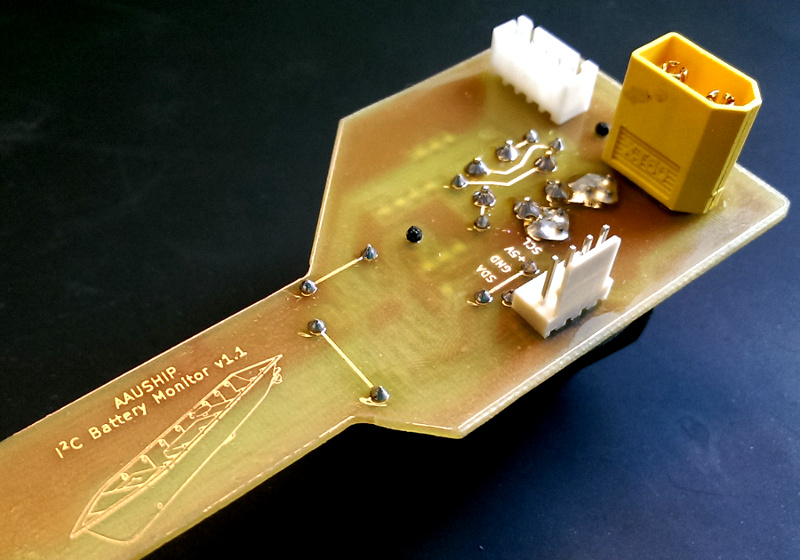
\includegraphics[width=0.8\textwidth]{fig/bm-macro}
	\caption{Macro photo of the finished battery monitor.}
	\label{fig:bm-macro}
\end{figure}

\begin{figure}[H]
	\centering
	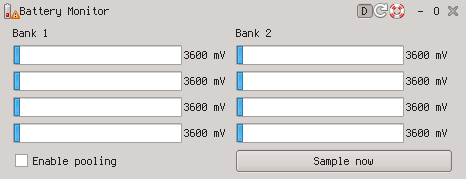
\includegraphics[width=\textwidth]{fig/bm-rqt}
	\caption{Screen shot of the battery monitor plugin in rqt.}
	\label{fig:bm-rqt}
\end{figure}

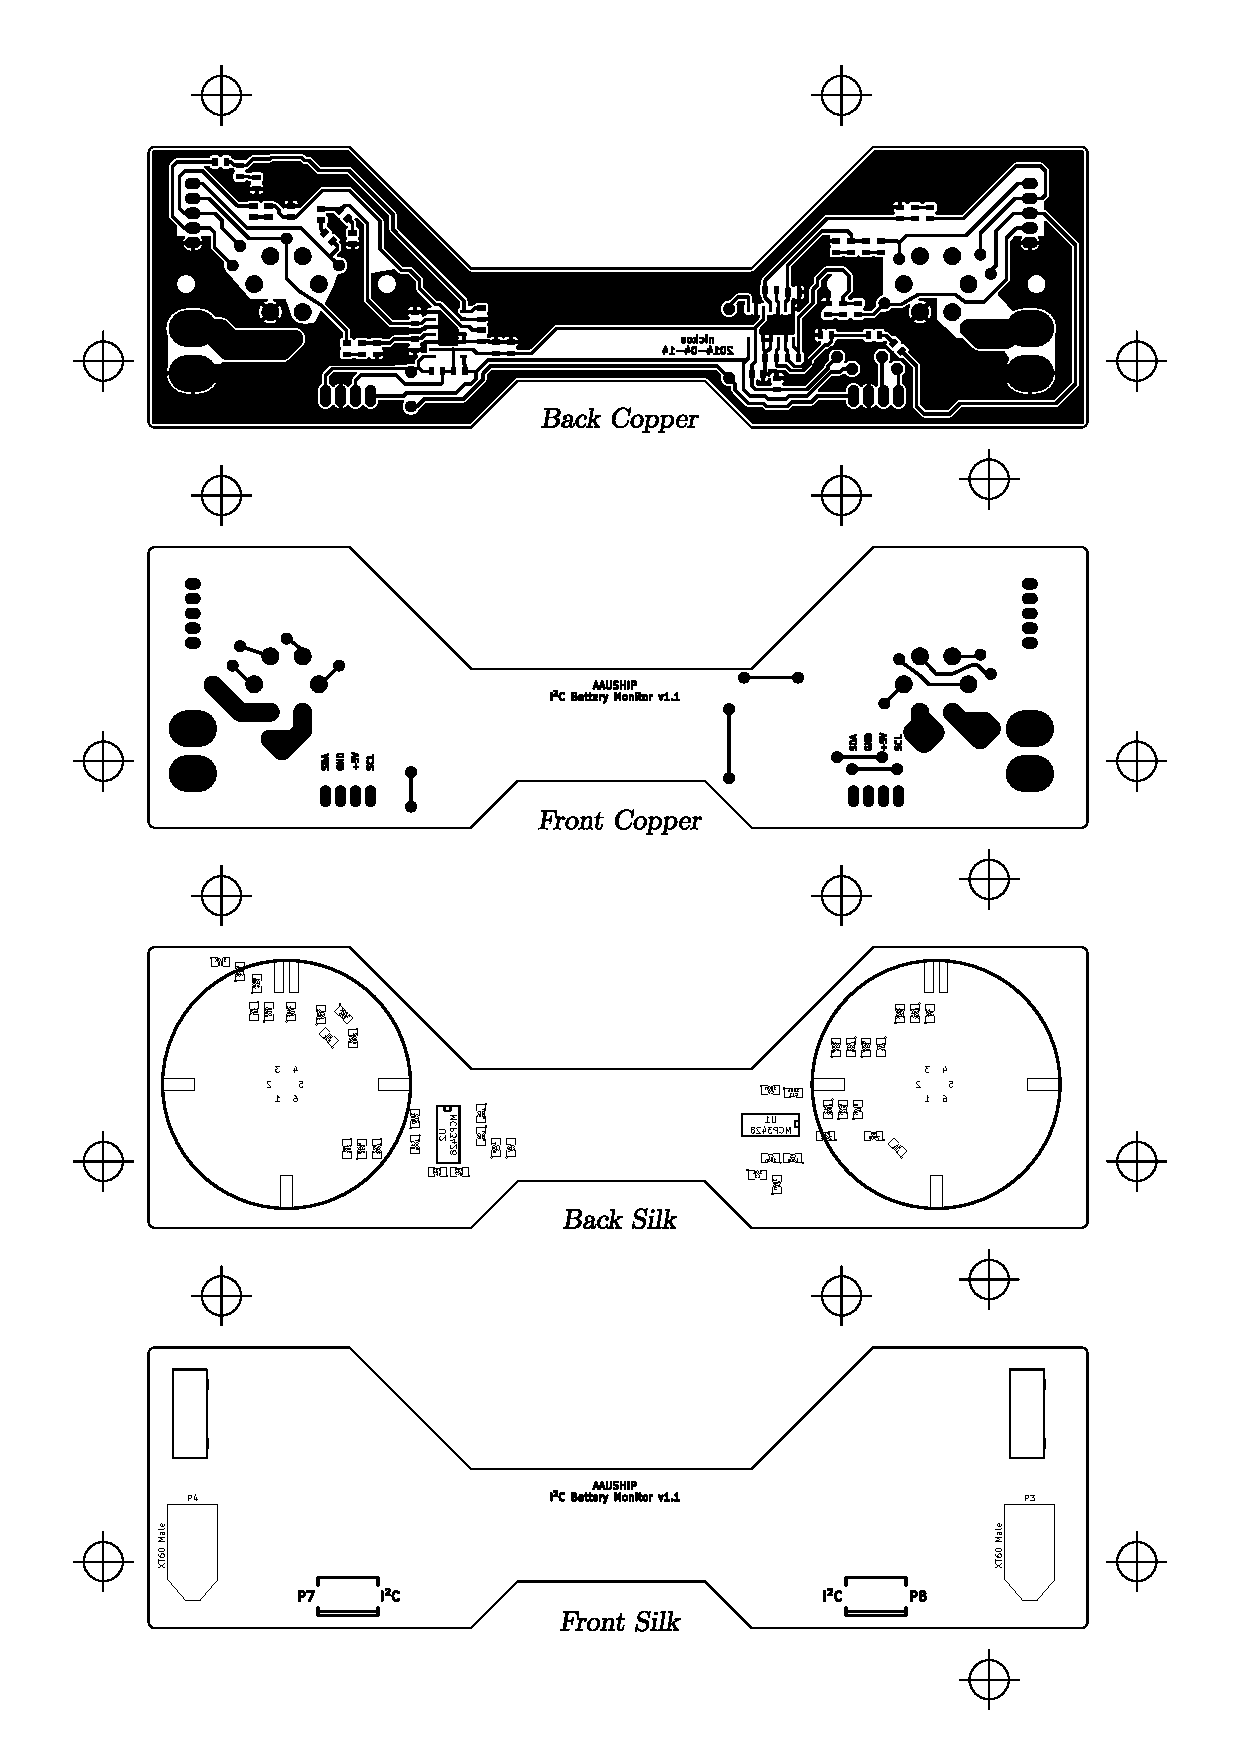
\includepdf{pdf/bm-pcb}
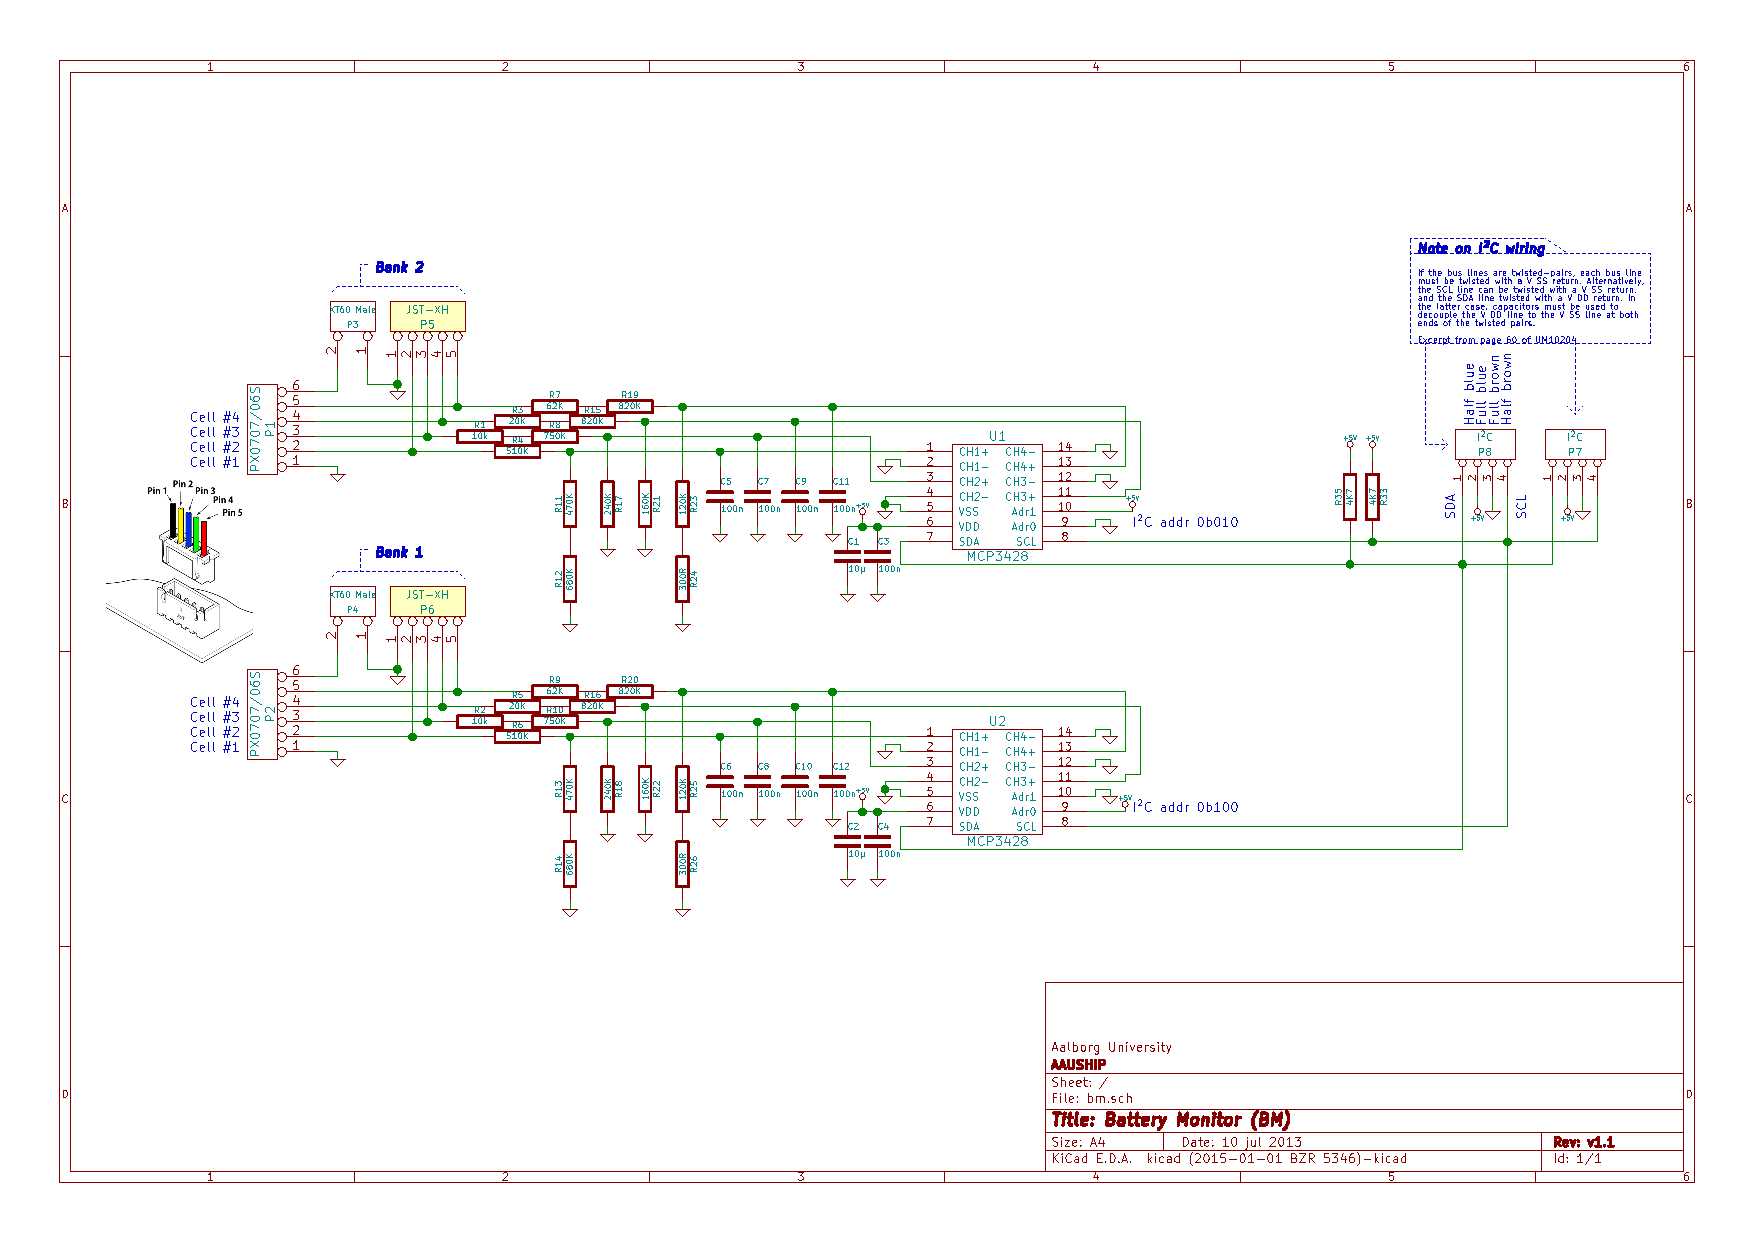
\includepdf[angle=90]{pdf/bm-sch}

%\chapter{Workshop Paper}
\label{ch:paper}

The following paper has been submitted to \textit{The 3rd AAU
Workshop on Robotics, 2014}.

\todo[inline]{\vspace{2cm}\\Remember to attach the paper on the
following pages\vspace{2cm}}





\backmatter
\bibliographystyle{apalike}
\bibliography{../manual/bib}
\label{ch:litt}

%\settocdepth{section}
\listoftodos
\end{document}

